%Nicht anfassen, so ist der Dokumentenaufbau
\documentclass[a4paper, 12pt]{article}
\usepackage[utf8]{inputenc} % Kodierung
\usepackage[T1]{fontenc} % Explizite Nennung des Fonts
%\usepackage{tgschola}
%\usepackage{utopia}
\usepackage{helvet}

\usepackage{xargs}                      % Use more than one optional parameter in a new commands
\usepackage[pdftex,dvipsnames]{xcolor}  % Coloured text etc.

% \usepackage[colorinlistoftodos,prependcaption,textsize=small]{todonotes}
\usepackage[disable]{todonotes}
\newcommandx{\unsure}[2][1=]{\todo[linecolor=red,backgroundcolor=red!25,bordercolor=red,#1]{#2}}
% \newcommandx{\change}[2][1=]{\todo[linecolor=blue,backgroundcolor=blue!25,bordercolor=blue,#1]{#2}}
% \newcommandx{\info}[2][1=]{\todo[linecolor=OliveGreen,backgroundcolor=OliveGreen!25,bordercolor=OliveGreen,#1]{#2}}
% \newcommandx{\improvement}[2][1=]{\todo[linecolor=Plum,backgroundcolor=Plum!25,bordercolor=Plum,#1]{#2}}
% \newcommandx{\thiswillnotshow}[2][1=]{\todo[disable,#1]{#2}}

%\renewcommand\familydefault{\sfdefault} 
\usepackage[english,ngerman]{babel} % Sprache %ngermen

\usepackage{datetime}
\newdateformat{myformat}{\THEDAY{. }\monthname[\THEMONTH] \THEYEAR}

\usepackage{graphicx} % immer benötigt für das Einbinden von Graphiken
\usepackage{caption} % Beschriftung von Bildern 
\captionsetup[sub]{font=small, labelfont=normalsize}
\usepackage[font=small]{subcaption}

\usepackage{blindtext} % Wenn man das Layout prüfen will, kann hier mit \blindtext Text eingefügt werden.

\usepackage{parskip} % Für den Abstand zwischen 2 Absätzen.
%\setlength{\parskip}{12pt plus80pt minus10pt} % Genaue Einstellung von parskip

\usepackage{lmodern}

%Literaturverzeichnis
\usepackage[style=trad-abbrv,backend=biber, backref=false]{biblatex}
 % Biber backend für Literaturverzeichnis
% \addbibresource{bibliography.bib} % Einbinden der Literatur.
%\DeclareLanguageMapping{english}{english-apa} % Anpassen Spracheinstellungen im Literaturverzeichnis.

\usepackage[activate={true,nocompatibility},
	final,
	tracking=true,
	kerning=true,
	expansion=true,
	spacing=true,
	factor=1050,
	stretch=25,
	shrink=10]{microtype} % Für die Feineinstellung der Zeichensetzung.

\usepackage[right=3 cm, left=3cm, top=2.5 cm, bottom=3 cm]{geometry} % Seitenränder
  \linespread{1.25}

\usepackage{appendix}
\usepackage{setspace}
\usepackage{fancyhdr} % Für schönere Kopf-/Fußzeilen und Fußnoten.
\pagestyle{fancy}
\setlength{\headheight}{14.49998pt}

\usepackage[rflt]{floatflt} % Bild in Text
\usepackage[]{graphicx} %Bilder %change draft to final
% \usepackage{subcaption} % Bildunterschrift
\usepackage{booktabs} % für Tabellen
\usepackage{pbox} % für Boxen
\usepackage{tabulary} %für Tabellen
\usepackage{comment} % für Kommentare 
\usepackage{amssymb}
% \usepackage[fleqn]{amsmath}
\usepackage{amsmath} 
% \usepackage{upgreek} 
% \let\mu\upmu 

\usepackage{mathtools}
\usepackage{mathrsfs}
\usepackage[nocomma,short]{optidef}
\usepackage{gensymb}

\usepackage{rotating}
\usepackage{makecell}
\usepackage{tabto}
\usepackage{beramono}

% \usepackage{minted}

\usepackage[nocomma,short]{optidef}
\newcommand*{\matr}[1]{\mathbf it{#1}}
\newcommand*{\tran}{^{\mkern-1.5mu\mathsf{T}}}

% \usepackage{mdframed}
\newtheorem{theorem}{Theorem}
\newtheorem{lemma}{Lemma}
\newtheorem{problem}{Problem}

\usepackage{verbatim} % Text ohne Formatierung ausgeben
\usepackage{fancyvrb} % Verbatim konfigurieren
\usepackage{csquotes} % Für ordentlichen Anführungszeichen

%\usepackage{floatpag} %suppress pagenumber
%\captionsetup[sub]{font=small,labelfont={bf,sf}}
% placing figure at top of page
\makeatletter
\setlength{\@fptop}{0pt}
\makeatother

\newcommand{\rom}[1]{\uppercase\expandafter{\romannumeral #1\relax}}

\usepackage{hyperref}
% \usepackage[hidelinks]{hyperref} % Klickbare aber nicht markierte Links im PDF
\hypersetup{colorlinks={true},linkcolor={blue},urlcolor=blue, citecolor=black, anchorcolor=blue}
\usepackage[capitalise,noabbrev,nameinlink]{cleveref} 
\usepackage{nameref}
\Crefname{problem}{Problem}{Problems}
\crefname{problem}{Problem}{Problems}
\Crefname{constraint}{Constraint}{Constraints}
\crefname{constraint}{Constraint}{Constraints}
\Crefname{table}{Table}{Tables}
\crefdefaultlabelformat{(#2#1#3)}
% \creflabelformat{problem}{#2\textup{#1}#3}
\creflabelformat{section}{#2\textup{#1}#3}
\creflabelformat{theorem}{#2\textup{#1}#3}
\creflabelformat{figure}{#2\textup{#1}#3}
\creflabelformat{algorithm}{#2\textup{#1}#3}
\creflabelformat{table}{#2\textup{#1}#3}
\creflabelformat{apptab}{#2\textup{#1}#3}
\creflabelformat{chapter}{#2\textup{#1}#3}

\counterwithout{table}{chapter}
\counterwithout{figure}{chapter}

\crefname{appfig}{Appendix Figure}{Appendix Figures}
\crefname{apptab}{Appendix Table}{Appendix Tables}
\Crefname{appfig}{Appendix Figure}{Appendix Figures}
\Crefname{apptab}{Appendix Table}{Appendix Tables}

% \creflabelformat{constraint}{#2\textup{#1}#3}
% \creflabelformat{equation}{#2\textup{#1}#3}
\crefrangelabelformat{constraint}{(#3#1#4--#5\crefstripprefix{#1}{#2}#6)}

% \usepackage{algorithmicx}
\usepackage{algorithm}% http://ctan.org/pkg/algorithms
\usepackage{algpseudocode}% http://ctan.org/pkg/algorithmicx

\usepackage{makecell}
\renewcommand\theadalign{bc}
\renewcommand\theadfont{\bfseries}

\usepackage{float}

\newcommand{\RomanNumeralCaps}[1]{\MakeUppercase{\romannumeral #1}}

\usepackage{chngcntr}
% \counterwithin{figure}{subsection}
% \counterwithin{table}{section}
% \counterwithin{equation}{section}

\usepackage[nottoc]{tocbibind}% load before tocbasic
\usepackage[titles]{tocloft}
\usepackage{tocbasic}
\usepackage{scrbase}
\renewcommand*{\tableofcontents}{\listoftoc[{\contentsname}]{toc}}
% \renewcommand*{\listoffigures}{\listoftoc[{\listfigurename}]{lof}}
% \renewcommand{\cftloftitlefont}{\hfill\large\bfseries}
\renewcommand*{\listoftables}{\listoftoc[{\listtablename}]{lot}}
\cftsetindents{figure}{1.5em}{3.5em}

% \renewcommand\listoffigures{%
%     \section{\listfigurename}% Used to be \section*{\listfigurename}
%       \@mkboth{\MakeUppercase\listfigurename}%
%               {\MakeUppercase\listfigurename}%
%     \@starttoc{lof}%
%     }

\makeatletter
\newcommand\renewlistof[3]%
   {\renewcommand#1%
      {\section*{#3}%
      %  \addcontentsline{toc}{chapter}{#3}%
       \markboth{#3}{#3}%
       \@starttoc{#2}%
      }%
   }
\makeatother
\renewlistof\listoffigures{lof}{\listfigurename}

\DeclareNewTOC[
  type=myequation,
  name=Equation,
  listname={\large List of Equations},
  tocentrynumwidth=2.3em,% like figures and tables
  tocentryindent=1.5em,% like figures and tables
]{equ}
\newcommand{\myequations}[1]{%
  \addxcontentsline{equ}{myequation}[\theequation]{#1}}
\setuptoc{equ}{leveldown,totoc}

\DeclareNewTOC[
  type=myproblem,
  name=Problem,
  listname={\Large List of Problems},
  tocentrynumwidth=2.3em,% like figures and tables
  tocentryindent=1.5em,% like figures and tables
]{pro}
\newcommand{\myproblems}[1]{%
%   \addxcontentsline{pro}{myproblem}[\theproblem]{#1}}
  \addcontentsline{pro}{myproblem}{#1}}
\setuptoc{pro}{leveldown}
\counterwithout{equation}{chapter}

% \usepackage{tocloft}
% \usepackage[titles]{tocloft}
% \newcommand{\listequationsname}{List of Equations}
% \newlistof{myequations}{equ}{\listequationsname}
% \newcommand{\myequations}[1]{%
% \addcontentsline{equ}{myequations}{\protect\numberline{\theequation}#1}\par}

% \newcommand{\listproblemname}{List of Mathematical Programs}
% \newlistof{myproblems}{pro}{\listproblemsname}
% \newcommand{\myproblems}[1]{%
% \addcontentsline{pro}{myproblems}{\protect\numberline{\theproblem}#1}\par}

\usepackage{enumitem}
\usepackage{acro}

\usepackage{changepage}

\usepackage{etoolbox}
\robustify{\label}

\usepackage{setspace}

\usepackage{pdfpages}
\DeclareAcronym{lp}{
  short=LP,
  long=linear program,
}

\DeclareAcronym{dp}{
  short=DP,
  long=disjunctive program,
}

\DeclareAcronym{mip}{
  short=MIP,
  long=mixed-integer program,
}

\DeclareAcronym{fba}{
  short=FBA,
  long=flux balance analysis,
}

\DeclareAcronym{ll-fba}{
  short=ll-FBA,
  long=loopless FBA,
}

\DeclareAcronym{mp}{
  short=MP,
  long=master problem,
}

\DeclareAcronym{sp}{
  short=SP,
  long=subproblem,
}


\DeclareAcronym{mis}{
  short=MIS,
  long=minimal infeasible subsystem,
}

\DeclareAcronym{gem}{
  short=GEM,
  long=genome-scale metabolic model,
}

\DeclareAcronym{cobra}{
  short=COBRA,
  long=constraint-based resconstruction and analysis,
}

\DeclareAcronym{cff}{
  short=CFF,
  long=CycleFreeFlux,
}


\acsetup{make-links}
\newcommand\acfi[2][]{\acf[#1,format/long=\itshape]{#2}}

% \sloppy
\fancyhf{}
\rfoot{\thepage}
\renewcommand{\headrulewidth}{0pt}
%Special cells with linebreaks possible
\newcommand{\specialcell}[2][c]{%
	\begin{tabular}[#1]{@{}t@{}}#2\end{tabular}}
%define blockquote-quotation environment
\renewenvironment{quotation}{
	\leftskip1cm
	\rightskip1cm
	\noindent
	\setstretch{1}
	\small
}

% define Footnote
\renewcommand\footnoterule{\kern-3pt \hrule width 3in height 0.7pt \hskip3pt \kern 2.6pt}
\let\oldfootnote\footnote
\renewcommand\footnote[1]{%
	\oldfootnote{\hspace{2mm}#1}}
%%%%%

% microtyping around some characters

%Extra-spacing around dash, and quotation-marks, and parentheses
\SetExtraKerning[unit=space]
	{
		encoding={*}, family={qhv}, series={b}, size={normalsize,large,Large}
	}
	{
		\textendash={400,400}, % for double-dash
		\textquotedblleft={ ,120}, % for left quotation-mark
		\textquotedblright={170, }, % for right quotation-mark
		"28={ ,250}, % left bracket, add space from right
		"29={300, } % right bracket, add space from left
	}

%%%%%


\makeatletter
\newcommand{\MSonehalfspacing}{%
  \setstretch{1.44}%  default
  \ifcase \@ptsize \relax % 10pt
    \setstretch {1.448}%
  \or % 11pt
    \setstretch {1.399}%
  \or % 12pt
    \setstretch {1.433}%
  \fi
}
\newcommand{\MSdoublespacing}{%
  \setstretch {1.92}%  default
  \ifcase \@ptsize \relax % 10pt
    \setstretch {1.936}%
  \or % 11pt
    \setstretch {1.866}%
  \or % 12pt
    \setstretch {1.902}%
  \fi
}
\newcommand{\MSverbatimspacing}{%
  \setstretch{1.44}%  default
  \ifcase \@ptsize \relax % 10pt
    \setstretch {1}%
  \or % 11pt
    \setstretch {1}%
  \or % 12pt
    \setstretch {1}%
  \fi
}
\makeatother


\addbibresource{bibliography.bib}

\begin{document}
\selectlanguage{english}

\newgeometry{margin=2.5cm}
\begin{titlepage}
\thispagestyle{empty}
\newcommand{\HRule}{\rule{\linewidth}{0.5mm}}
\hspace{1cm}
\center

{\huge Freie Universität Berlin}\\[1.0cm]
{\Large Fachbereich Mathematik und Informatik}\\[0.8cm]
% {Dahlem Center for Machine Learning and Robotics}\\[4.0cm] 

% {\huge Masterarbeit}\\[1.0cm]

%\HRule\\[1.4cm]

{ \huge \bfseries Integer Optimization for loopless \\ Flux Balance Analysis }\\[4cm]
%{ \large }\\[0.3cm] % Falls nicht benötigt, einfach auskommentieren
%\HRule \\[2.4cm]
{\textit{Hannah Marie Troppens}}\\
{Matrikelnummer: 5039637}\\
{hannah.troppens@fu-berlin.de}\\[1cm]
% {Betreuer: Prof. Dr. Tim Landgraf}\\
% {1. Gutachter: Prof. Dr. Tim Landgraf}\\
% {2. Gutachter: Prof. Dr. Dr. habil. Raúl Rojas }

\vspace{1cm}
% \begin{otherlanguage}{ngerman}
\myformat{\today}
% \end{otherlanguage}
\end{titlepage}
\restoregeometry


%%%%%%%%%%%%%%%%%%%%%%%%%%%%%
%%%Ab hier Inhalt einfügen%%%
%%%%%%%%%%%%%%%%%%%%%%%%%%%%%

\pagenumbering{roman}
\newpage
\section*{\centering Abstract}

Loopless Flux Balance Analysis (ll-FBA) is a constraint-based approach to predict flux distributions in cells that do not contain internal loops, which would be physiologically unrealistic.
ll-FBA is a disjunctive program, usually reformulated as a mixed-integer program, and is challenging to solve for biological models that often contain thousands of reactions and metabolites. \\
In this thesis, we compare various reformulations of ll-FBA and different solution approaches. We discuss the use of intersection cuts and compare the performance of blocking cycles to decomposing the problem and to solving the convex-hull formulation.\\
Overall, the combinatorial Benders' decomposition is the most promising of the tested approaches with which we could solve most instances. However, the model size and numerical instability pose a challenge to the combinatorial Benders' method.
\section*{\centering Zusammenfassung}

Loopless Flux Balance Analysis (ll-FBA) ist eine Constraint-basierte Methode zur Modellierung des Stoffwechsels in der Zelle.
ll-FBA ist ein disjunktives Programm, das in der Regel als gemischt-ganzzahliges Programm umformuliert wird, und ist für biologische Modelle, die oft Tausende von Reaktionen und Metaboliten enthalten, schwierig zu lösen. \\
In dieser Arbeit vergleichen wir mehrere Umformulierungen von ll-FBA und unterschiedliche Lösungsstrategien. Wir erörtern die Verwendung von Schnittebenen basierend auf Schnittstellen und testen die Laufzeit, wenn thermodynamisch unmögliche Lösungen durch Ungleichungen von dem Lösungsraum abgeschnitten werden. Außerdem vergleichen wir die Laufzeit, wenn ll-FBA in zwei Teilprobleme zerlegt wird, und wenn wir das Problem so umformulieren, dass wir die konvexe Hülle des disjunktiven Programms erhalten.\\
Insgesamt ist die kombinatorische Benders-Zerlegung der vielversprechendste der getesteten Ansätze, mit dem wir die meisten Instanzen lösen. 
Allerdings stellen die Größe des Models
und die numerische Instabilität eine Herausforderung für die kombinatorische Benders Methode dar.



\newpage
% Inhaltsverzeichnis
\thispagestyle{plain}
\setstretch{1.25} % Zeilenabstand
\microtypesetup{protrusion=false}
\tableofcontents
\microtypesetup{protrusion=true}
\thispagestyle{plain} % Kein Header aber mit Seitenanzahl

\newpage
\pagestyle{fancy}
\fancyhead{} % Clears the standard fancy style
\fancyhead[R]{\rightmark} %Kopfzeile rechts
% \fancyhead[L]{\leftmark}
% \fancyhead[L]{\rmshape\nouppercase{\leftmark}} %Kopfzeile links

\setstretch{1.25}
\clearpage
\thispagestyle{plain}
\section*{Abbreviations}

% \todo[inline]{future work: improve cut, separation}
% \todo[inline]{constraint handler}
% possible extension to st FBA
% exact LP
% \todo[inline]{move numerically tricky part to LP (MIS search), could use exact LP to MIS search to deal with numerical instability}
\listoffigures
\listofmyproblems
\todo[inline]{add standard form, primal and dual problem}
% \listoftables
% \listofalgorithms
% \listofmyequations

% \todo[inline]{use caption and subcaption in figures/ tables}
\todo[inline]{fix figure counter}
% \unsure[inline]{list of equations? list of problems?}
\newpage
\pagenumbering{arabic}
\thispagestyle{plain}
\section{Introduction}

In systems biology, biological systems are modelled mathematically in order to predict the behaviour of the system \cite{intro_computational_systems_biology}. An important and fundamental system is the cell and its metabolism.
Due to advances in technology, detailed information about different cells and organisms is available. Based on this data, genome-scale models can be constructed. Metabolic networks are genome-scale models which capture the interactions between entities in the cell such as small molecules (metabolites) and enzymes~\cite{intro_computational_systems_biology}. 
A commonly used approach to study metabolic networks are constraint-based methods, where we assume a steady-state of metabolites within the cell, which means that the production and consumption of each metabolite is balanced \cite{palsson_systems_biology}. The steady-state assumption, together with bounds on the flux through each reaction, defines a system of linear constraints. A solution corresponds to the flux distribution, which is the rate of each reaction, that satisfies the constraints \cite{intro_computational_systems_biology}. \\ %flow of metabolites through a metabolic network using mathematical optimization
A basic method to analyse the flux distribution in a metabolic network is flux balance analysis (FBA) \cite{FBA}. In FBA, a linear program is solved where we optimise a biological objective function, such as maximising growth. As cells evolve under selection pressure, it is plausible that the behaviour is in line with a biological objective and using mathematical optimization to study the flow of metabolites through a metabolic network is reasonable \cite{palsson_systems_biology}. With FBA it is possible to predict cellular behaviour in accordance with observations in experiments \cite{FBA}. \\
%% MOTIVATION AND CONTEXT 1-2 pages
%% get attention and introduce topic
%% background information
% \todo[inline]{question addressed system biology}
% System biologists model large biological systems with the help of mathematical approaches to predict the behaviour of the system \cite{intro_computational_systems_biology}. 
% \todo[inline]{goal of modelling}
% \todo[inline]{question addressed with studying metabolic models} 
% \todo[inline]{metabolic models}
% \todo[inline]{availability of GEMs}
% Due to advances in technology, 
% quantitative data on biological systems.... detailed information of the cell ...
% We have access to the composition of ... give rise to reconstructed biochemical reaction networks \cite{palsson_systems_biology}.
% \todo[inline]{metabolic network}
% \todo[inline]{FBA} 
% Flux balance analysis is an approach for analyzing the flow of metabolites through a metabolic network using mathematical optimization \cite{FBA}.
% \todo[inline]{success and use of FBA}
% \todo[inline]{problems with FBA}
However, solutions of FBA often violate the loop law, which means that the solution contains internal cycles which is biologically not plausible. Loopless FBA (ll-FBA) is an extension to FBA which includes thermodynamic information \cite{elimination_infeasible_loops}. A solution to ll-FBA does not contain internal cycles, but ll-FBA is computationally harder as we need to solve a disjunctive program, which is usually reformulated as a mixed-integer program (MIP). 
In this thesis, we look at different reformulations of ll-FBA and compare the performance of different MIP techniques. \todo[inline]{MIP technique correct for all/most approaches?}

%% thesis statement: topic, question being addressed, summarize resulst and significance
%% STRATEGY 1 page: what am I trying to do

%% OUTLINE 1/2 page
%% and outlines structure to come
% \todo[inline]{overview of thesis}

In \cref{section:optimization}, we will give a short introduction into mathematical optimization and present the aspects relevant for this thesis including the concept and solving strategies for linear programming, mixed-integer programming and disjunctive programming. In \cref{section:metabolic_networks}, we will motivate the biological context in more detail and present the relevant constrained-based methods in detail. 
The methods used are presented in \cref{section:methods} including a combinatorial Benders' approach and intersection cuts for ll-FBA. In \cref{section:results}, we present and discuss the computational results. 

\todo[inline]{FBA extensions}

\thispagestyle{plain}
\section*{Preliminaries and Notation}
% \todo[inline]{use variables consistently; which words to write in italic}

\begin{enumerate}
    % \item The set $\mathbb{R}$ denotes the set of real numbers and the set $\mathbb{Z}$ denotes the set of whole numbers. If scalar $\alpha$ is in the set of real numbers, we write $\alpha \in \mathbb R$. \todo[inline]{remove?} %(instead of $\mathbb R ^1$) 
    
    \item A vector $\bold{v} = (v_1, ..., v_n) \in \mathbb{R}^n$ is identified as a column vector and printed in bold. The transpose of $\mathbf v$ into a row vector is written as $\mathbf v^\intercal$. The inner product of two vectors $\mathbf v, \mathbf w \in \mathbb{R}^n$ is $\mathbf v^\intercal \mathbf w = \sum_{i=1}^n v_i w_i$. With $\mathbf v \leq \mathbf w$ we denote element-wise inequality. With $\ln (\mathbf v)$ we denote the element-wise natural logarithm. 
    The 1-vector is written as $\mathbf 1 := (1, 1, ..., 1) \in \mathbb{R}^n$ the 0-vector as $\mathbf 0 := (0, 0, ..., 0) \in \mathbb{R}^n$. The \textit{support} of $\bold{v}$ is the set of indices $i$ with $v_i \neq 0$ and is denoted by $\text{supp}(\mathbf v)$. With $\text{sign}(\mathbf v)$ the element-wise sign function is applied to $\bold v$.
    The concatenation of two vectors $\mathbf x$, $\mathbf y$ is denoted by $(\mathbf x, \mathbf y)$.

    \item The entry in row $i$ and column $j$ of a matrix $ \mathbf A \in \mathbb{R}^{m \times n}$ is denoted by $a_{i,j}$. The $i$-th row is $\boldsymbol a_{i,*}$ and the $j$-th column $\boldsymbol a_{*,j}$. %\todo[inline]{update in entire section, often one index used for row of matrix} 
    The zero matrix is denoted by $\mathbf 0_{m,n}$ with $m$ rows and $n$ columns. With $\text{diag}(\mathbf v)$ we denote the quadratic matrix with $\mathbf v$ on the diagonal and 0 for all other entries.
    
    \item The \textit{rank} of the matrix $\mathbf A \in \mathbb{R}^{m \times n}$ corresponds to the number of linearly independent columns of $\mathbf A$ and is denoted by $\text{rank}(\mathbf A)$. The matrix $\mathbf A$ is said to be of \textit{full rank} if $\text{rank}(\mathbf A) = \min \{ m, n\}$. The number of linearly independent rows and linearly independent columns is always equal.
    % \todo[inline]{sufficient to say rank(A) is rank of matrix?}
    
    \item Let $\mathbf A \in \mathbb{R}^{n \times n}$ be an invertible matrix: $ \mathbf A \mathbf A^{-1} = \mathbf I$, where $\mathbf I$ is the identity matrix. The matrix $ \mathbf A^{-1}$ is the inverse matrix of $ \mathbf A$. %\todo[inline]{when is matrix invertible}
    $\mathbf I_n$ is the $n \times n$ identity matrix.

    \item A \textit{linear combination} is defined as $\sum_{i=1}^{m} \lambda_i \mathbf x_i = 
    \lambda_i x_1 + ... + \lambda_m x_m$, where $\lambda_i \in \mathbb{R}$ and $x_i \in \mathbb{R}^n$.
    A line going through a point $\mathbf x$ generated by $\mathbf r \in \mathbb{R}^n$ is the set $\{\mathbf x + \lambda \mathbf r | \lambda \in \mathbb{R}\}$. A \textit{line segment} is a subset of a line defined on the interval between $l \in \mathbb{R}$ and $u \in \mathbb{R}$: $\{\mathbf x + \lambda \mathbf r | \lambda \in \mathbb{R}, \, \lambda \in [l, u ]\}$.

    \item A \textit{basis} $B$ of a vector space $V$ is a set of vectors $(\mathbf v_1, \mathbf v_2, ..., \mathbf v_n)$ that are linearly independent and every $\mathbf v \in V$ can be written as a linear combination of vectors in $B$.

    \item The \textit{nullspace} of a matrix $\mathbf A \in \mathbb{R}^{m \times n}$ is defined as $\text{null}(\mathbf A):=\{\mathbf x \in \mathbb{R}^n: \mathbf A \mathbf x = ~\mathbf0\}$. 
    \vspace*{-\baselineskip}
    
    \newpage
    \item A set $C \subseteq \mathbb{R}^n$ is \textit{convex} if for any two points $\mathbf x, \mathbf y \in C$ the line segment between $\mathbf x$ and $\mathbf y$ is in $C$. %every convex combination for any two points $x,y \in X$ is contained in $C$.
    The \textit{convex hull} of a set $X$ is the smallest convex set that contains all points in $X$ and is denoted by $\text{conv}(X)$. It is a set of convex combinations such that all points $x_i$ in $X$ can be represented, where a \textit{convex combination} is a linear combination with $\lambda_i \geq 0$ and $\sum_{i=1}^m \lambda_i = 1$.
    % \todo[inline]{D: should be proper definition?}

    \item The set $\{\mathbf x \in \mathbb{R}^n | \boldsymbol \alpha^\intercal \mathbf x = \boldsymbol \beta \}$ is a \textit{hyperplane}, where $\boldsymbol \alpha \in \mathbb{R}^n$ and $\boldsymbol \beta \in \mathbb{R}$. The set $\{\mathbf x \in \mathbb{R}^n | \boldsymbol \alpha^\intercal x \leq \boldsymbol \beta \}$ is a \textit{half-space}. %\cite{understanding_lp}
    A \textit{polyhedron} $P = \{ \mathbf x \in \mathbb{R}^n | \mathbf A \mathbf x \leq \mathbf b\}$ is the intersection of a finite number of half-spaces, where $\mathbf A \in \mathbb{R}^{m \times n}$ and $\mathbf b \in \mathbb{R}^m$. Hyperplanes, half-spaces and polyhedra are convex. A point $\mathbf x \in P$ is an \textit{extreme point} or \textit{vertex} if it cannot be represented as a convex combination of any set of other points in $P$. %\todo[inline]{closed halfspace needed?} 
    A \textit{polytope} is a bounded polyhedron if there exists a large enough ball in which it can be placed \cite{understanding_lp}.
    % can be written as the convex hull of the extreme points of $P$. 
    % \todo[inline]{verify}
    % \todo[inline]{add reference}

    \item A set $C \subseteq \mathbb{R}^n$ is a \textit{cone} if $\lambda \mathbf x \in C$ for any $\mathbf x \in C$ and $\lambda \geq 0$. A \textit{conic combination} is a linear combination with $\lambda_i \geq 0$. %A cone is a \textit{convex cone} if it contains the conic combinations of all $x_i \in C$. 
    $C$ is \textit{pointed} if it contains no line and the extreme point is called $apex$. A nonzero vector $\mathbf r \in \mathbb{R}^n$ is a \textit{ray} of $C$ if $\{\mathbf x + \lambda \mathbf r | \lambda \geq 0 \} \in C$ for any $\mathbf x \in C$. Ray $\mathbf r$ is an \textit{extreme ray} if it cannot be represented by a conic combination of other rays in $C$. 
    A cone is $polyhedral$ if the number of extreme rays is finite. A cone is \textit{simplicial} if it has $n$ extreme rays \cite{bienstock_outer_product_free_sets}. 
    The \textit{conic relaxation} of an extreme point $\mathbf x$ of a polyhedron $P$ is a cone with apex $\mathbf x$, and the extreme rays are the half-spaces of $P$ intersecting at $\mathbf x$.
    
    % \unsure[inline]{how to define ray, as r as lambda r or as x + lambda r}
    \item A set $S \subseteq \mathbb{R}^n$ is \textit{open} if for any point $\mathbf x \in S$ there exists an $\epsilon > 0$ such that the ball centered at $\mathbf x$ with radius $\epsilon$ is contained in $S$. A set is \textit{closed} if its complement is open. 
    % A set is \textit{closed} if it contains all its boundary points. 
    In particular, the set of whole numbers $\mathbb{Z} \subseteq \mathbb{R}$ is closed.
    % \item Let $S \in \mathbb{R}^n$ be a nonempty set and $\mathbf x$ a point in $S$. $\mathbf x$ is in the \textit{interior} of $S$, denoted by $\text{int}(S)$, if there exists an $\epsilon > 0$ such that any point in the ball centered at $\mathbf x$ with radius $\epsilon$ is contained in $S$. 
    % $\mathbf x$ is on the \textit{boundary} of $S$, denoted by $\text{bd}(S)$, if it is not in $\text{int}(S)$. 
    % $S$ is \textit{closed} if the boundary of $S$ is contained in $S$, $S$ is said to be \textit{open} otherwise. %https://wiki.math.ntnu.no/linearmethods/basicspaces/openandclosed
    % % \todo[inline]{does ball have to be open? subset of euclidean space.\\MB: you can specify if you consider balls as closed or open by default. People use open ball and closed ball explicitly when it matters.}
    % This also holds if the boundary is the empty set and therefore $\mathbb{Z}$ is closed.
    % \todo[inline]{should be definition for open, and closed is complement of open set}
\end{enumerate}
\thispagestyle{plain}


\newpage
\thispagestyle{plain}
\section{Mathematical Optimization} \label{section:optimization}
\todo[inline]{brief introduction as in Huibert's thesis, shorten intro section, refer to book}
\todo[inline]{link to other sections}
Optimization appears in various disciplines. 
In timetabling, we seek a schedule at school such that teachers are assigned to students at a given time \cite{timetabling}. Of course different requirements have to be satisfied. Each teacher and student should have only one class at a time. The classes should not be too big and the teachers are only allowed to teach a limited number of hours per week. 
Another example for an optimization problem is clustering, where we want to divide a set of data points into subsets that share similarities \cite{clustering}. 
Optimization also arises in nature. Animals adapt and optimize their behaviour through learning \cite{optimization_systems_biology}.
Even the behaviour in cells can be modelled by mathematical optimization with biological objectives such as maximizing growth or minimizing energy usage which could be traits evolutionary selected for \cite{intro_computational_systems_biology}. Optimization in cells is the topic of this thesis and we will see in \cref{section:metabolic_networks} how to use mathematical optimization to answer questions arising in systems biology.
\todo[inline]{book Palsson, objective functions in practice; plus page 5 for evolution}

In mathematical optimization, the goal is to find an optimal solution that respects requirements that arise in our application. In order to represent a problem in practice by a mathematical model, we need to formulate an objective. An objective in timetabling could be minimizing the number of used classrooms, and in clustering an objective is to minimize the difference between the points in the same cluster. Additionally, we need to identify entities of the system. In timetabling, we would have students, teachers, rooms and time as different entities in the model. We also need to identify the constraints, i.e. the requirements in our system. Once the objective, the entities and the requirements of a system are identified, it can be expressed mathematically.
The resulting model is an \textit{optimization problem}, and we can use optimization algorithms to compute solutions. 
We define an optimization problem as:
\begin{mini!}
    {\scriptstyle \bold x \in \mathbb{R}^n}{f(\bold x)}{ \label[problem]{problem:optimization_problem}}{}
    \addConstraint{g_i(\bold x) \leq 0, \quad i=1,...,m} 
\end{mini!}

\quad where $f$ is the \textit{objective function}, $g_i$ are the \textit{constraint functions} and $\bold x$ are the \textit{decision variables}. %\cite{boyd_stephen_convex_2004}
The \textit{feasible region} is the set of points that respect the constraints. An optimization problem with a constrained feasible region is often also called \textit{constrained optimization problem} in contrast to an \textit{unconstrained optimization problem}. A \textit{solution} is a vector $\bold x$ that lies in the feasible region. An \textit{optimal solution} $\bold x^*$ is a solution with the smallest objective value. The \textit{objective value} of $\bold x^*$ is the value of the objective function evaluated at $\bold x^*$. If a problem has no solution, meaning that the constraints cannot be satisfied simultaneously, it is said to be \textit{infeasible}. A problem is \textit{unbounded} if solutions exist, but the objective value can be arbitrarily small.
One can maximize a function $f$ by setting the objective function to $\min -f(\bold x)$.

Depending on the type of the objective function and the type of constraints, optimization problems are divided into different classes. The classes relevant for this thesis are linear programs, mixed-integer programs and disjunctive programs\footnote[1]{Program in this context does not mean a computer program. The term was coined in the 1950s and referred to planning in a military context. See \cite{understanding_lp} for more detail.}. 
Different algorithms can be used to solve optimization problems, which depend on the problem structure.
% \todo[inline]{or define solution as optimal solution}

\subsection{Linear Programming} \label{section:Linear Programming}
A \acfi{lp} is an optimization problem with a linear objective function and linear constraints.

\begin{mini!}
    {\scriptstyle \bold x}{\bold c^\intercal \bold x}{\text{\textbf{LP}} \label[problem]{problem:LP}}{}
    \addConstraint{\bold A \bold x\leq \bold b} 
    \addConstraint{\bold x \in \mathbb{R}^n}
    % \addConstraint{x\geq \bold 0} 
\end{mini!}

\quad where $\bold c \in \mathbb{R}^n$, $ \bold A \in \mathbb{R}^{m \times n}$ and $\bold b \in \mathbb{R}^m$. It is assumed that the number of constraints $m$ is greater or equal to the number of variables $n$. %\unsure[inline]{to have an \textit{underdetermined} system of linear equations which allows to have many solutions} \todo[inline]{there can be many solutions regardless: e.g. a half space -> many solutions (M.)} 
We also assume that the columns of $\bold A$ are linearly independent.\todo[inline]{ok?}
The linear inequalities define a polyhedron. If an optimal solution exists and if the feasible region has vertices\todo[inline]{necessary?}, there exists an optimal solution at one of the vertices. \todo[inline]{double check with reference \\ what if we just have one line on which the optimum lies? Per definition not unbounded but solution not at extreme point} In that case, the LP can have exactly one optimal solution or multiple optimal solutions, for example if an entire edge or face is optimal. An LP has no optimal solution if it is infeasible or unbounded.
\cref{problem:LP} is said to be in \textit{inequality form}%\unsure[inline]{ok to do so without constraints on x?} 
\cite{boyd_stephen_convex_2004}.

As an example, we want to solve the following optimization problem: 
\begin{maxi!}
    {\scriptstyle x, y}{y}{ \label[problem]{problem:lp_example}}{}
    \addConstraint{0 \leq x \leq 3} 
    \addConstraint{0.5 \leq y \leq 4} 
    \addConstraint{y \leq 1.5 x + 0.5} 
    \addConstraint{y \leq -0.5 x + 4.5}
    \addConstraint{x,y \in \mathbb{R}}
\end{maxi!}
% \begin{equation} \label[problem]{problem:lp_example}
%     \text{max} \{y \, : \, 0 \leq x \leq 3 , \, 0.5 \leq y \leq 4, \, y \leq 1.5 x + 0.5, \, y \leq -0.5 x + 4.5, \, x,y \in \mathbb{R} \}
% \end{equation} 
The decision variables $x, y$ are continuous. We want to find a solution $(x^*, y^*)$ with maximal $y$-value such that the constraints are respected. The problem is a linear program and can be written as \cref{problem:LP} by simple linear transformations. If we want to write \cref{problem:lp_example} as a minimization problem, the objective becomes $-y$. If we visualise the example (\cref{fig:lp}), we see that there exists one optimal solution located at $(2,3.5)$. Usually, we are interested in problems in higher dimensions and it is not possible to solve them visually.
\todo[inline]{mention non-degeneracy?}
% \todo[inline]{why orthogonal line to objective function has the same objective values}

\begin{figure}[h!]
    \centering
    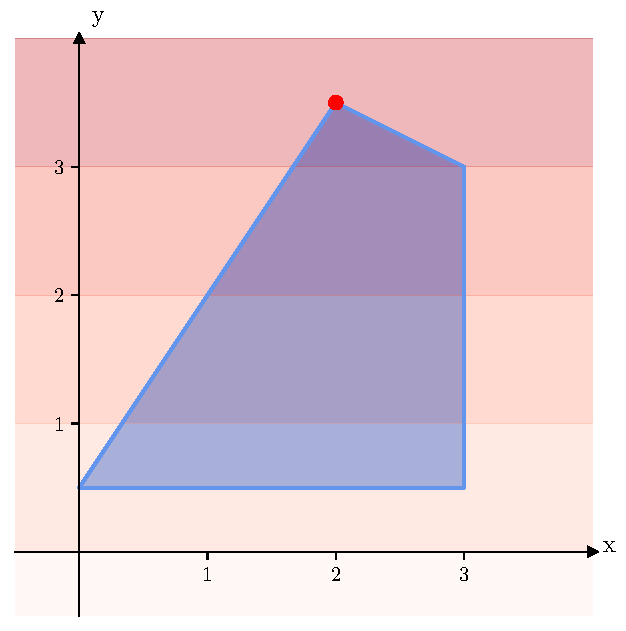
\includegraphics[width=0.6\textwidth]{Images/lp.pdf}
    \caption{\label{fig:lp} Visualization of LP (\cref{problem:lp_example})}
    \subcaption*{
        The set of feasible solutions contains all the points in the interior or on the boundary of the polytope (blue line segments). The optimal solution is the point in the feasible region with the biggest $y$-value (red point). The isolines indicate the function value of the points.}
\end{figure} \unsure[inline]{remove grid?}

An LP is said to be in \textit{standard form} if it is of the form:
\begin{mini!}
    {\scriptstyle x}{\bold c^\intercal \bold x}{\label[problem]{problem:LP_standard_form}}{}
    \addConstraint{\bold A \bold x = \bold b} 
    \addConstraint{\bold x \geq \bold 0} 
\end{mini!}

\quad where $\bold c, \bold x \in \mathbb{R}^n, \, \bold A \in \mathbb{R}^{m \times n}$ and $\bold b \in \mathbb{R}^m$. 
\cref{problem:LP} can be written in standard form by adding one \textit{slack variable} per inequality to write it as equality \cite{noauthor_numerical_2006}. $\bold a_{i,*}^\intercal \bold x \leq b_i$ becomes $\bold a_{i,*} \,^\intercal \bold x + s_i = b_i$ with $s_i \geq 0$. Each variable $x_i$ that can be negative is replaced by $x_i^+ - x_i^-$, where $x_i^+ \geq 0$ and $x_i^- \geq 0$ \cite{noauthor_numerical_2006}.

A vertex of the feasible region is also called \textit{basic feasible solution}. Suppose we have an LP in standard form as in \cref{problem:LP_standard_form} with linearly independent rows. Let $\bold x \in \mathbb{R}^n$ be a basic feasible solution. There exist $n$ constraints that are a basis defining $\bold x$. $B$ is the set of constraint indices that are in the basis. Any variable $x_i \in B$ is a \textit{basic variable}. A variable $x_i \not \in B$ is a \textit{nonbasic variable} and $x_i=0$ \cite{understanding_lp}. \todo[inline]{verify why constraint indices !!!}

\subsubsection{Solving LPs} \label{section:solving_lps}
There exist several algorithms to solve linear programs. The \textit{ellipsoid method} is the first algorithm that was proven to have a polynomial running time in the worst case. However, in practice, other algorithms outperform it \cite{understanding_lp}. Another class of algorithms are \textit{interior-point methods}. Some interior-point methods have a polynomial running time in the worst case and are often used in practice. Interior-point methods start with a feasible solution in the interior of the feasible region and approach the optimum without stepping outside the feasible region \cite{understanding_lp}. \\
Another algorithm that is relevant in practice is the \textit{simplex algorithm}. It is based on the fundamental property of LPs that the optimum is located at one of the vertices of the feasible region. %\todo[inline]{and that each vertex is corresponds to a basis, wrong words (M.)}. 
In \textit{phase \RomanNumeralCaps{1}} of the algorithm, a vertex of the feasible region is computed. In \textit{phase \RomanNumeralCaps{2}}, the algorithm moves from vertex to vertex along edges of the feasible region until an optimum is found. The \textit{pivot rule} determines to which vertex the algorithm moves next. There exist several pivot rules, however for all of them, there are families of problem instances on which the number of pivot steps needed grows exponentially. The worst case running time on some instances is in conflict with the observed polynomial running time in practice. Studying the simplex method with \textit{smoothed analysis}, which tries to close this gap, shows a polynomial running time of the simplex method. In smoothed analysis, a small noise is added to the entries of a fixed instance and afterwards worst-case analysis is performed on the perturbed instance \cite{huiberts,dadush}.
% \todo[inline]{when which algorithm is better}

\subsubsection{Optimality and Duality}
% \todo[inline]{transition}
To prove that a solution is optimal, we can use the \textit{Karush-Kuhn-Tucker}-conditions (KKT-conditions) and see the relation between the primal and the dual problems in LPs. 
An optimization problem can be written as an unconstrained problem by augmenting the objective function with a weighted sum of the constraints \cite{boyd_stephen_convex_2004}. The resulting function is known as the \textit{Lagrangian} function.
The Lagrangian of an LP in standard form is \cite{noauthor_numerical_2006}: 
\begin{equation} \label{Eq:lagrangian}
\mathcal{L} (\bold x, \boldsymbol{\lambda}, \boldsymbol \nu) = \bold c^\intercal \bold x - \sum_{i=1}^n \lambda_i x_i - \sum_{i=1}^m \bold \nu_i (A_{i,*}^\intercal \bold x - b_i)
\end{equation} %\todo[inline]{$\lambda_i (x_i)$ correct?}
\quad where $\lambda_i \geq 0$ and $\nu_i \in \mathbb{R}$ are called \textit{Lagrange multipliers} or \textit{dual variables}.
As the objective function of linear programs is convex, the KKT-conditions are a proof for global optimality of a solution. We obtain the optimality conditions captured in \cref{theorem:lp_duality}. 

\newpage
\begin{theorem}[Optimality conditions for LPs] \label{theorem:lp_duality}
    A solution $\bold x^*$ is optimal if there exist vectors $\boldsymbol \lambda$ and $\boldsymbol \nu$ that satisfy the following conditions \cite{noauthor_numerical_2006}:
    \begin{enumerate}
        \item $\boldsymbol \lambda + \bold A^\intercal \boldsymbol \nu = \bold c $ \hfill (stationarity)
        \item $ \bold A \bold x - \bold b = \bold 0$ \hfill (primal feasibility)
        \item $\bold x \geq \bold 0$ \hfill (primal feasibility)
        \item $\boldsymbol \lambda \geq \bold 0$ \hfill (dual feasibility)
        \item $\bold x^\intercal \boldsymbol \lambda = \bold 0$ \hfill (complementary slackness)
    \end{enumerate}
\end{theorem} 
We call a linear program in standard form as in \cref{problem:LP_standard_form} the \textit{primal problem} ($\mathcal{P}$).
The associated \textit{dual function} of the primal problem is \cite{aps_mosek_nodate, boyd_stephen_convex_2004}:
\todo[inline]{MB: shouldn't the conditions $x \geq 0, \lambda \geq 0$ appear somewhere?}
\begin{align*}
    q(\boldsymbol \lambda, \boldsymbol \nu)
    & = \inf_{\bold x} \mathcal{L} (\bold x, \boldsymbol \lambda, \boldsymbol \nu) \\
    & = \inf_{\bold x} \bold c^\intercal \bold x - \boldsymbol \lambda^\intercal \bold x - \boldsymbol \nu^\intercal (\bold A \bold x - \bold b) & \\
    & = \inf_{\bold x} \bold c^\intercal \bold x - \boldsymbol \lambda^\intercal \bold x - \boldsymbol \nu^\intercal \bold A \bold x + \boldsymbol \nu^\intercal \bold b  &\\
    & = \inf_{\bold x} (\bold c^\intercal - \boldsymbol \lambda^\intercal - \boldsymbol \nu^\intercal \bold A) \bold x + \boldsymbol \nu^\intercal \bold b  &\\
    & = \inf_{\bold x} \bold x^\intercal (\bold c - \boldsymbol \lambda - \bold A^\intercal \boldsymbol \nu) + \bold b^\intercal \boldsymbol \nu &\\
    & = \left\{
    \begin{array}{lr}
        \bold b^\intercal \boldsymbol \nu \quad \quad \text{if} \, \, \bold c - \boldsymbol \lambda - \bold A^\intercal \boldsymbol \nu = \bold 0\\
        - \infty \quad \quad \text{otherwise}
    \end{array}
    \right.
\end{align*}

% \todo[inline]{check if it has to be inf}
Let $\bold x^P$ be a feasible solution to the primal problem, and let $(\boldsymbol \lambda^D, \, \boldsymbol \nu^D)$ be a feasible solution to the dual problem. If the dual function is bounded we know that $\bold c - \boldsymbol \lambda^D = \bold A^\intercal \boldsymbol \nu^D$ and we know that $\bold x^P$ satisfies $ \bold A\bold x^P = \bold b$. The function value $q(\boldsymbol \lambda^D, \boldsymbol \nu^D)$ is a lower bound on the objective value of the primal problem \cite{aps_mosek_nodate}: 
\begin{equation*}
    \bold b^\intercal \boldsymbol \nu^D
    = (\bold A \bold x^P)^\intercal \boldsymbol \nu^D 
    = \bold {x^P}^\intercal \bold A^\intercal \boldsymbol \nu^D 
    = \bold {x^P}^\intercal (\bold c - \boldsymbol \lambda^D) 
    = \bold c^\intercal \bold x^P  - \boldsymbol {\lambda^D}^\intercal \bold x^P
    \leq \bold c^\intercal \bold x^P
\end{equation*}
The tightest bound maximizes $\bold b^\intercal \boldsymbol \nu$. Formulated as a linear program we obtain the \textit{dual problem} ($\mathcal{D}$):
\begin{maxi!}
    {\scriptstyle \boldsymbol \nu, \boldsymbol \lambda}{\bold b^\intercal \boldsymbol \nu}{\label[problem]{problem:dual_problem_slack}}{}
    \addConstraint{\boldsymbol \lambda + \bold A^\intercal \boldsymbol \nu = \bold c} 
    \addConstraint{\boldsymbol \lambda \geq \bold 0} 
\end{maxi!}
or rewritten without the slack variables $\boldsymbol \lambda$ \cite{noauthor_numerical_2006}:
\begin{maxi!}
    {\scriptstyle \boldsymbol \nu}{\bold b^\intercal \boldsymbol \nu}{\label[problem]{problem:dual_problem}}{}
    \addConstraint{\boldsymbol A^\intercal \boldsymbol \nu \leq \bold c} 
\end{maxi!}
% \unsure[inline]{add dimensions to all variables}
Let $p^*$ be the objective value of an optimal solution for the primal problem and $d^*$ the objective value of an optimal solution to the dual problem. We have seen that $d^*$ is a lower bound on $p^*$ which is known as \textit{weak duality}. We speak of \textit{strong duality} if $p^*=d^*$. 

\begin{theorem}[Strong Duality] \label{theorem:strong_duality}
    Given a primal $\mathcal{P}$ and corresponding dual program $\mathcal{D}$, exactly one of the following is true \cite{noauthor_numerical_2006}:
    \begin{enumerate}
        \item $\mathcal{P}$ and $\mathcal{D}$ both have at least one optimal solution. If $p^*$ is the objective value of an optimal solution to $\mathcal{P}$ and $d^*$ is the objective value of an optimal solution to $\mathcal{D}$, then $p^*=d^*$.
        \item Either $\mathcal{P}$ or $\mathcal{D}$ is unbounded and the other is infeasible. 
        \item $\mathcal{P}$ and $\mathcal{D}$ both are infeasible.
    \end{enumerate}
\end{theorem}
% For linear programs, \textit{strong duality} holds. 
A proof for \cref{theorem:strong_duality} can be found in \cite{aps_mosek_nodate}. Property (1) of \cref{theorem:strong_duality} can be used to prove the optimality of a solution. 

We have seen how to derive the dual problem of an LP in standard form. We do not require an LP in standard form to derive the corresponding dual problem. For example, the dual problem of \cref{problem:LP} is: 
\begin{maxi!}
    {\scriptstyle \boldsymbol \mu}{\bold b^\intercal \boldsymbol{\mu}}{\label[problem]{problem:LP_dual}}{}
    \addConstraint{\bold A^\intercal \boldsymbol{\mu} = \bold c} 
    \addConstraint{\mu_i \geq 0}
    % \addConstraint{x\geq \bold 0} 
\end{maxi!}

% \todo[inline]{example + visualization}
% \begin{lemma}[Farkas Lemma]
%     Given an LP in standard form, exactly one of the following is true:
%     \begin{enumerate}
%         \item the LP has at least one solution $x$
%         \item there exists a vector $y$ such that $ \bold A^\intercal y \leq 0$ and $b^\intercal y > 0$
%     \end{enumerate}
% \end{lemma}

% \cite{aps_mosek_nodate}

\subsection{Mixed-Integer Programming} \label{section:MIP}
Many problems in practice cannot be formulated by only using linear constraints and continuous decision variables. It is often required that a subset of variables is discrete. A \acfi{mip} is an optimization problem with a linear objective function, linear constraints and a subset of integer variables:

\begin{mini!}
    {\scriptstyle \bold x}{\bold c^\intercal \bold x}{\text{\textbf{MIP}} \label[problem]{problem:MIP}}{}
    \addConstraint{\bold A \bold x\leq \bold b} \label[constraint]{constraint:MIP_inequality}
    % \addConstraint{x\geq \bold 0} 
    \addConstraint{\bold x \in \mathbb{Z}^{|J|} \times \mathbb{R}^{n-|J|} \label[constraint]{constraint:MIP_integer}
    }
\end{mini!}

\quad where $\bold c \in \mathbb{R}^n, \, \bold A \in \mathbb{R}^{m \times n}$, $\bold b \in \mathbb{R}^m$. The set $J$ contains the indices of integer variables. 

Let us reuse the LP example in \cref{section:Linear Programming} and add integrality constraints on the decision variables $x$ and $y$:
\begin{maxi!}
    {\scriptstyle x, y}{y}{ \label[problem]{problem:mip_example}}{}
    \addConstraint{0 \leq x \leq 3} 
    \addConstraint{0.5 \leq y \leq 4} 
    \addConstraint{y \leq 1.5 x + 0.5} 
    \addConstraint{y \leq -0.5 x + 4.5}
    \addConstraint{x,y \in \mathbb{Z}}
\end{maxi!}
% \begin{equation} \label[problem]{problem:mip_example}
%     \text{max} \{y \, : \, 0 \leq x \leq 3 , \, 0.5 \leq y \leq 4, \, y \leq 1.5 x + 0.5, \, y \leq -0.5 x + 4.5, \, x,y \in \mathbb{Z} \}
% \end{equation} 

Looking at the visualisation of the problem (\cref{fig:mip}), we see that the optimal solution of the LP $x^{LP} = (2,3.5)$ is no valid solution for the MIP formulation. The points $(2,3)$ and $(3,3)$ are the optimal solutions.

\begin{figure}[h!]
    \centering
    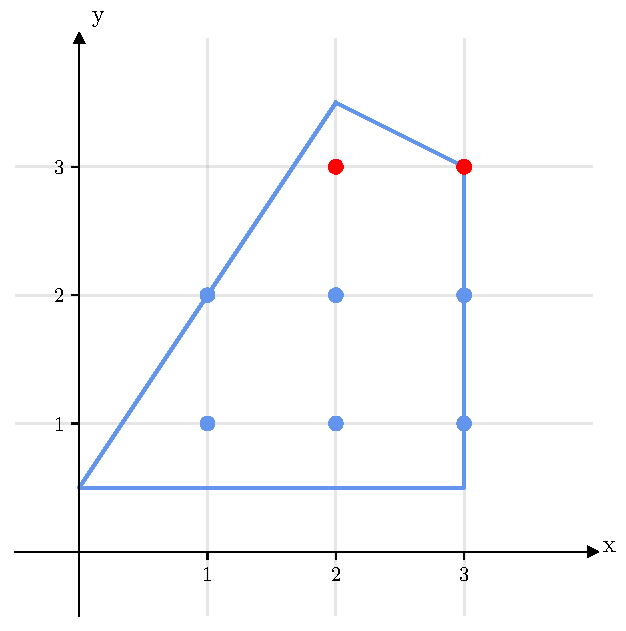
\includegraphics[width=0.6\textwidth]{Images/mip.pdf}
    \caption{Visualisation of MIP (\cref{problem:mip_example})}
    \label{fig:mip}
    \subcaption*{
        The feasible points of the MIP are the integer points respecting the polyhedral constraints (blue points). The set of feasible solutions to the relaxed LP is are all the points in the interior or on the boundary of the polytope (blue line segments). An optimal solution is a point in the feasible region with the biggest $y$-value (red point). The optimal solutions are at $(2,3)$ and $(3,3)$.}
\end{figure}

The MIP formulation enables us to model much more complex problems. Apart from incorporating discrete quantities, it is possible to capture Boolean expressions. Suppose we want to model the \textit{indicator constraint} $z = 1 \implies \bold a^\intercal \bold x \leq b$. We can reformulate the constraint with a linear constraint using the \textit{big-M method}: 
\begin{equation*}
    \bold a^\intercal \bold x \leq b + M(1-z)
\end{equation*}
If $z=1$ the constraint is enforced. In the case $z=0$, the value of $M$ has to be larger than $\bold a^\intercal \bold x - b$ for any $\bold x$ such that the constraint is inactive \cite{aps_mosek_nodate}.

\subsubsection*{Solving MIPs} \addcontentsline{toc}{subsubsection}{\protect\numberline{}Solving MIPs}
Solving MIPs is much more complicated than solving LPs, because it is not guaranteed that if an optimal solution exists, it is at one of the vertices. In general, solving MIPs is $\mathcal{NP}$-hard. A problem is in $\mathcal{NP}$ if the solution is verifiable in polynomial time. A problem is $\mathcal{NP}$-hard if it requires at least as much time to solve the problem as any other problem that is $\mathcal{NP}$-complete. $\mathcal{NP}$-complete problems are $\mathcal{NP}$-hard and are in $\mathcal{NP}$ \cite{CormenIntroduction}. In complexity theory, problems are defined as decision problems. 
The decision problem of \cref{problem:MIP} would be "Is the feasible region nonempty?", which is $\mathcal{NP}$-complete. As finding an optimal solution is not easier than finding any solution, it follows that MIPs are $\mathcal{NP}$-hard \cite{integer_programming}.
% NP: set of decision problems solvable in polynomial time and verifiable in polynomial time 
% NP-hard: polynomial time reduction from an NP-complete problem G to H -> H can be optimization problem
% 0-1 integer linear programmings is NP-complete
% MILP feasibility problem is in NP:
% - yes verifiable in polynomial time
% - 
\todo[inline]{verify correctness, add reduction}
% Achtung! NP-hard problems müssen nicht zwangsweise Decision Problems sein, NP und NP-complete problems aber schon!
% Inbesondere muss sich ein NP-hard problem auf ein NP-completes problem (in poly zeit) reduzieren lassen, ergo wenn ich einen polynomischen Lösungansatz für das zweite habe, habe ich auch einen für das erste.

Instead of solving the MIP directly, one can solve a sequence of \textit{LP relaxations}: the integrality constraints are ignored and \cref{constraint:MIP_integer} becomes $\bold x \in \mathbb{R}^n$.
Let $z^{LP}$ be the objective value of an optimal solution $\bold{x}^{LP}$ of the LP relaxation and $z^*$ the objective value of an optimal solution $\bold{x^*}$ to the MIP problem. We know that: 
\begin{equation*} \label{Eq:bound}
    z^{LP} \leq z^*
\end{equation*}
One common approach for solving MIPs is the \textit{branch-and-bound} algorithm \cite{integer_programming}. The idea is to generate a branch-and-bound tree starting with the solution to the LP relaxation $\bold x^{LP} \in \mathbb{R}^n$ at the root node. A variable $x_i$ that is fractional in $\bold x^{LP}$ and violates the integrality constraint is selected as \textit{branching variable}. We divide the search space $P$ by creating two child nodes. In one $x_i$ has to be larger or equal to the ceiled value and the feasible region becomes $P \cap \{x_i \geq \lceil x_i^{LP} \rceil \}$. In the other child node, $x_i$ can take at most the floored value of $x_i^{LP}$ and the feasible region of the subproblem is $P \cap \{x_i \leq \lfloor x_i^{LP} \rfloor \}$. The solution with the smallest objective value respecting the MIP formulation is called \textit{incumbent} and the objective value is denoted by $z^{INC}$. We continue branching until all variables in $J$ are integral, a subproblem is infeasible or if a node can be $pruned$. The optimal solution in each node $i$ is bounded by the objective value of the relaxed solution $z^{LP}_{(i)}$. If $z^{LP}_{(i)}$ is greater or equal to $z^{INC}$, node $i$ is cut off the tree. \\
Another approach to solve MIPs is the \textit{cutting plane} algorithm \cite{integer_programming}. The LP relaxation can be very weak. As we are dealing with a linear objective, we could get the optimal MIP solution easily if we had access to the \textit{integer hull}: $\text{conv}(P \cap \mathbb{Z}^n)$. If the LP relaxation does not correspond to the integer hull, one can tighten the LP relaxation by adding \textit{cuts}. A cut is an inequality that does not cut off any feasible solution (see \cref{section:cuts}). Given an optimal solution to the LP relaxation $\bold x^{LP}$ that violates at least one integer constraint, one separates $\bold x^{LP}$ from the hull with a cut. This process is repeated until $\bold x^{LP}$ is an optimal solution to the MIP. \\
A combination of the branch-and-bound algorithm and the cutting plane algorithm is the \textit{branch-and-cut} algorithm \cite{integer_programming}. The LP relaxation at a node is potentially tightened by adding cuts. 

\subsection{Disjunctive Programming}
% \todo[inline]{motivation from MIP to DP}
Often, the requirements of a problem are complex, and linear constraints are not sufficient for the mathematical program. With Boolean expressions, more complicated relationships between variables can be captured without using the big-M formulation.     
A \acfi{dp} is an optimization problem with linear constraints, continuous variables and logical constraints:

\begin{mini!}
    {\scriptstyle \bold x}{\bold c^\intercal \bold x}{\text{\textbf{DP}} \label[problem]{problem:DP}}{}
    \addConstraint{\bold A \bold x\leq \bold b} 
    \addConstraint{\bigvee_{i \in Q_j} \{\bold d^{(i)\intercal} \bold x \leq d_{0}^i\} \quad \forall j \in S} 
\end{mini!}

\quad where $\bold c, \bold x \in \mathbb{R}^n$, $ \bold A \in \mathbb{R}^{m \times n}$ and $\bold b \in \mathbb{R}^m$. $\bold d^{(i)} \in \mathbb{R}^n, \, d_{0}^i \in \mathbb{R}$ and $S$ is the set of disjunction indices.
As the terms $i$ in each disjunction $Q_j$ are linear, each disjunctive set is a polyhedron. The feasible region is in general non-convex due to the disjunctive constraints \cite{balas_disjunctive_2018}.
Alternatively, the disjunctions can be captured by Boolean variables $Y_{ij} \in \{true, false \}$, where $Y_{ij}$ corresponds to the $i$-th disjunct in disjunction $j$:
\begin{mini!}
    {\scriptstyle \bold x}{\bold c^\intercal \bold x}{\label[problem]{problem:DP_bool}}{}
    \addConstraint{\bold A \bold x\leq \bold b} 
    \addConstraint{\bigvee_{i \in Q_j} \left[ \begin{array}{c}  
        Y_{ij}\\ 
        \{\bold d^{(i)\intercal} \bold x \leq d_{0}^i\}
    \end{array} \right] \quad \forall j \in S} 
    \addConstraint{\Omega (Y) = true}
\end{mini!}

As an example, we want to solve the following optimization problem:
% \begin{align} 
%     \begin{split}
%     \text{max} \{y \, : \, &((0 \leq x \leq 1) \land (0.5 \leq y \leq 1.5 x + 0.5)) \, \lor \\ &((2 \leq x \leq 3) \land (0.5 \leq y \leq -0.5 x + 4.5))  \, x,y \in \mathbb{R} \}
%     \end{split}
% \end{align} 
\begin{maxi!}
    {\scriptstyle x, y}{y}{\label[problem]{problem:dp_example}}{}
    \addConstraint{\begin{aligned}((0 \leq x \leq 1) \land (0.5 \leq y \leq 1.5 x + 0.5)) \, \, \lor \\ ((2 \leq x \leq 3) \land (2 \leq y \leq -0.5 x + 4.5)) \end{aligned}} 
    \addConstraint{x,y \in \mathbb{R}} 
\end{maxi!}

The feasible region is the union of two polyhedra and no longer convex. The optimal solution is the point with maximal value in either of the polytopes and located at $(2, 3.5)$ which we see in the visualization (\cref{fig:dp}). 

\begin{figure}[h!]
    \centering
    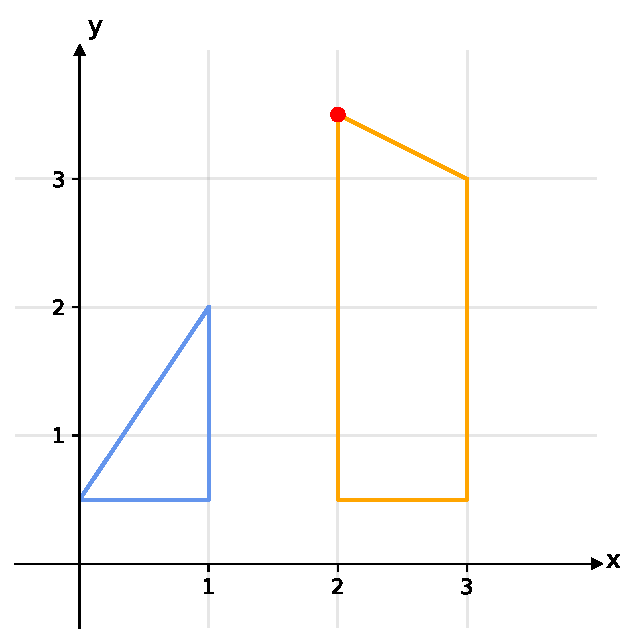
\includegraphics[width=0.6\textwidth]{Images/dp.pdf}
    \caption{Visualization of DP (\cref{problem:dp_example})}
    \label{fig:dp}
    \subcaption*{
        The set of feasible solutions is no longer convex and is the union of the polytope $P_1$ (blue line segments) and the polytope $P_2$ (orange line segments). The optimal solution is the point in the feasible region with the biggest $y$-value (red point).}
\end{figure}
% \unsure[inline]{write problem in dp form?}

\subsubsection*{Solving DPs} \addcontentsline{toc}{subsubsection}{\protect\numberline{}Solving DPs} \label{section:solving_dps}
\todo[inline]{mention big-M only in half sentence, DPs offer a different type of constraint, align with intro to DPs}
A disjunctive model can be formulated as mixed-integer program and solved by corresponding techniques (see \cref{section:MIP}). Disjunctions can be expressed by linear constraints and integer variables by using the big-M method. Suppose we have a disjunction with $k$ terms:
\begin{equation*}
    (\bold a_1^\intercal \bold x \leq b_1) \lor (\bold a_2^\intercal \bold x \leq b_2) ... \lor (\bold a_k^\intercal \bold x \leq b_k)
\end{equation*}
We use the binary variable $y_i$ and enforce with the constraint $y_1 +  y_2 + ... + y_k \geq 1$ that at least one of the $k$ terms is true. If $y_i=1$, term $(\bold a_i^\intercal \bold x \leq b_i)$ is enforced. See \cref{section:MIP} on how to express indicator constraints with linear constraints and binary variables. Often, the $M$ constant has to be large to be inactive if $y_i=0$. However, a large $M$ leads to a weaker LP relaxation which impacts the running time of the Branch-and-Bound algorithm \cite{aps_mosek_nodate}. 

Another possibility is to convexify the feasible region and solve the resulting linear program. The idea is to build the convex hull of the union of polyhedral points in a higher dimension. \todo[inline]{more details on higher dimension} The optimal solution at a vertex of the convex hull is optimal for the disjunctive program, as we are dealing with linear constraints. % and project the solution back to the original dimension of the problem. 
For an example on how to write a disjunctive program using the big-M or the hull reformulation, we refer to \cite{perez_disjunctiveprogrammingjl_2023}.
\cref{fig:dp_solving_techniques} shows the 2D-projection of the big-M reformulation and the convex-hull formulation of a disjunctive program. 

% \unsure[inline]{how to solve if corner can be infeasible?}
\begin{figure}[H]
    \centering
    \caption{DP reformulations}
    \label{fig:dp_solving_techniques}
    \begin{subfigure}{0.33\textwidth}
    \centering
        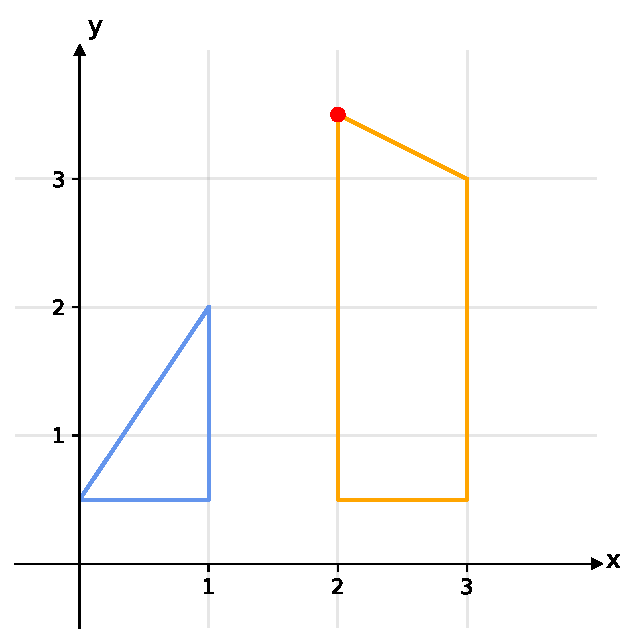
\includegraphics[width=0.95\linewidth]{Images/dp.pdf}
        \caption{}
    \end{subfigure}%
    \begin{subfigure}{0.33\textwidth}
    \centering
        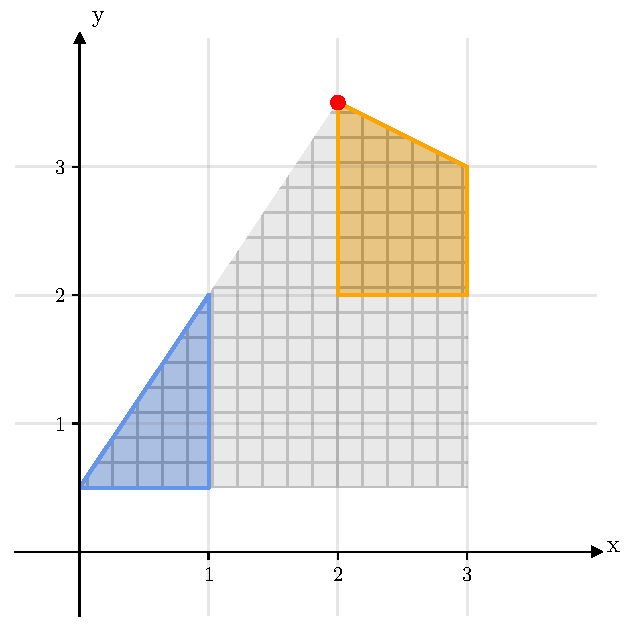
\includegraphics[width=0.95\linewidth]{Images/dp_big_m.pdf}
        \caption{}
    \end{subfigure}
    \begin{subfigure}{0.33\textwidth}
    \centering
        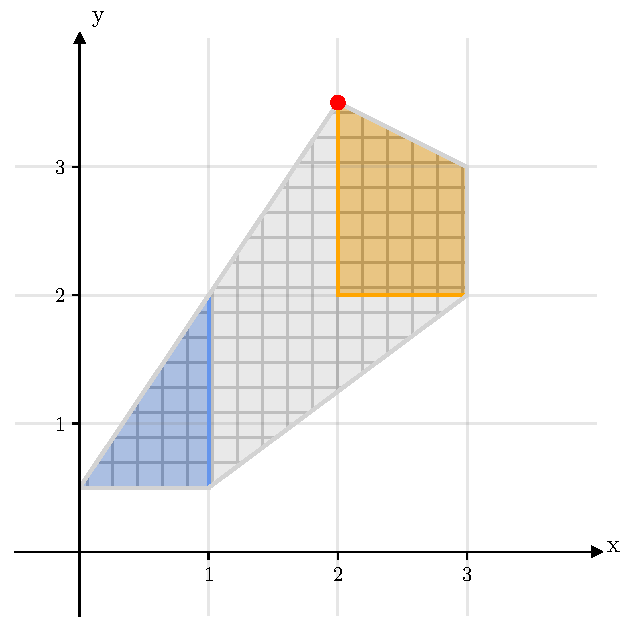
\includegraphics[width=0.95\linewidth]{Images/dp_convex_hull.pdf}
        \caption{}
    \end{subfigure}
    \subcaption*{The feasible region of a disjunctive program (a), the approximation of the region using the big-M reformulation (b) and the convex-hull reformulation (c). The plot is inspired by \cite{hutchison_automating_2010}.}
\end{figure}

\subsection{Decomposition and Cutting Planes} \label{section:cuts}
Let us consider a mixed-integer problem (\cref{problem:MIP}) with decision variables $\bold x$. A \textit{cutting plane} or \textit{cut}, parameterised by $\boldsymbol \alpha \in \mathbb{R}^{n+1}$, is an inequality that when added to the MIP does not remove any feasible solution, and is defined as: 
\begin{equation} \label{Eq:cuts}
    \sum_{i=1}^n \alpha_i x_i \leq \alpha_0 \quad  \forall \bold x \in P \cap S
\end{equation} 
\quad where $\alpha_i \in \mathbb{R}$, $P$ is the polyhedron defined by the inequality in \cref{constraint:MIP_inequality}, and $S$ is the set points satisfying \cref{constraint:MIP_integer}. Usually, cutting planes are used to cut off solutions to the relaxed problem that are infeasible in the original problem. 

\cref{fig:cuts} shows a visualisation of \cref{problem:mip_example} in which the optimal solution to the relaxed problem $\bold x^{LP}$ is not feasible in the MIP. $\bold x^{LP}$ is separated from the integer hull by cuts.

\begin{figure}[!h]
    \centering
    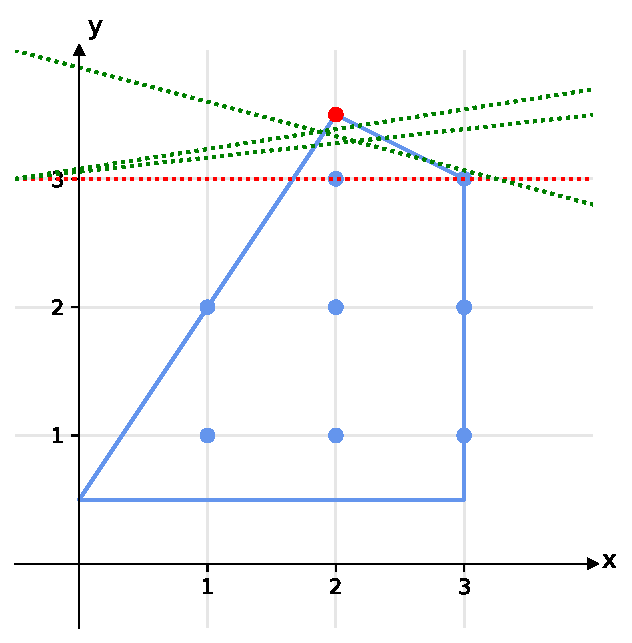
\includegraphics[width=0.6\textwidth]{Images/mip_cut.pdf}
    \caption{Tightening a relaxed problem with cuts (\cref{problem:mip_example})}
    \label{fig:cuts}
    \subcaption*{The feasible points of \cref{problem:mip_example} are the integer points within the polytope. In the relaxed problem, the integrality constraints are ignored. The optimal solution to the relaxed problem is $\bold x^{LP}=(2, 3.5)$. As $\bold x^{LP}$ is not an integer solution, it is cut off by adding cuts. The tightest cut is indicated by the red dashed line.}
\end{figure}
% \unsure[inline]{update caption, the relaxed problem is fix}

For a solution to the relaxed problem $\bold x^{LP}$ with $\bold x^{LP} \notin P \cap S$, there exist multiple hyperplanes separating $\bold x^{LP}$ from the actual feasible region. %\todo[inline]{MB: if you think of it, can there exists conditions where a unique hyperplane would separate a point from a convex set?}
As we want to tighten the search space, we are interested in cuts that cut off many infeasible points at once. There are different scores to estimate the quality of a cut \cite{turner_adaptive_2023}
. One scoring measure is \textit{efficacy} which is the signed distance from $\bold x^{LP}$ to the cutting plane:
\begin{equation}
    \text{eff}(\boldsymbol \alpha, \bold x^{LP}) := \frac{\boldsymbol \alpha^\intercal \bold x^{LP} - \alpha_0}{\lVert \boldsymbol \alpha \rVert}
\end{equation}

However, there is a tradeoff between the quality of a cut and the complexity of generating it.
\todo[inline]{differentiate between cut and decomposition}
The cuts relevant for this thesis are explained in detail below. 
\todo[inline]{numerical issues}

\todo[inline]{decomposition if variables of original problem are projected out; cut if we have a valid inequality \\
Decomposition for no-good cuts and combinatorial Benders'\\
intersection cuts are actual cuts}

\subsubsection{Decomposition with No-Good Cuts}
Given an integer problem P as in \cref{problem:MIP} with only binary variables: $J=n$ and $x_i \in \{0,1\}$. Let $\bold x^{IP}$ a solution to the relaxed integer program,  where \cref{constraint:MIP_inequality} is relaxed. 
If $\bold x^{IP}$ is not a feasible solution to P, we want to exclude the solution from the search space. The following \textit{no-good cut} is added to the relaxed IP and forbids the assignment of integer variables in $\bold x^{IP}$:
\begin{equation*}
    \sum_{j \in J: x_j^{IP}=0} (1 - x_{j}) + \sum_{j \in J: x_j^{IP}=1} x_j \quad \leq \quad |J| -1
\end{equation*}
Such a cut usually tightens the feasible region of P marginally and it would require a large number of no-good cuts to arrive at the integer hull.

\subsubsection{Combinatorial Benders' Decomposition} \label{section:optimization_CB}
Instead of forbidding one assignment of variables as with a no-good cut, with combinatorial Benders' cuts we generate stronger cuts, by identifying the subset of variables that lead to the infeasiblity. This section is based on \cite{codato_combinatorial_2006}.

Given a problem of the form:
\begin{mini!}
    {\scriptstyle \bold x, \bold z}{\bold c^\intercal \bold x}{\label[problem]{problem:mathematical_program_CB}}{} 
    \addConstraint{\bold F \bold x \leq \bold g}
    \addConstraint{\bold D \bold z \leq \bold e}
    \addConstraint{x_j = 1 \implies \bold a_{i,*}^\intercal \bold z \leq b_i \quad \forall i \in I} \label[constraint]{constraint:mathematical_program_CB_d}
    \addConstraint{x \in \{ 0,1 \}^n}
    \addConstraint{z_i \in \mathbb{R}}
\end{mini!} 
As the objective does not depend on $\bold z$ and as the decision variables $\bold x, \bold z$ are independent apart from the indicator constraints, we can split the problem into a \acfi{mp} and a \acfi{sp}. \cref{constraint:mathematical_program_CB_d} can be reformulated using the big-M method: $\bold A \bold z \leq \bold b + M(\bold 1- \bold x)$.

\begin{mini!}
    {\scriptstyle \bold x}{\bold c^\intercal \bold x}{\text{\textbf{MP}} \label[problem]{problem:MP}}{}
    \addConstraint{\bold F \bold x \leq \bold g}    
    \addConstraint{\bold x \in \mathbb{R}^n}
    \addConstraint{x_j \in \{ 0,1 \}}
\end{mini!}
The master problem ignores the constraints on $\bold z$. The subproblem depends on a solution $\bold x^{MP}$ to the master problem. 

\begin{mini!}
    {\scriptstyle \bold z}{0}{\text{\textbf{SP}} \label[problem]{problem:SP}}{}
    \addConstraint{\bold D \bold z \leq \bold e}
    \addConstraint{\bold a_{i,*}^\intercal \bold z \leq b_i + M(1- x_{j}^{MP}) \quad \forall i \in I}
\end{mini!}
% \unsure[inline]{write M as matrix, vector or constant}
If solution $\bold x^{MP}$ leads to a feasible subproblem, $\bold x^{MP}$ is an optimal solution to \cref{problem:mathematical_program_CB}. If the problem is infeasible, $\bold x^{MP}$ is not a feasible solution for the original problem. In that case we want to add a cut that removes $\bold x^{MP}$ from the search space. Suppose we have access to a \acfi{mis} $C$ that is an inclusion-wise minimal set of row indices corresponding to the constraints in the subproblem that lead to infeasibility.\\
The subproblem can then be written as:
\begin{mini!}
    {\scriptstyle \bold z}{0}{}{}
    \addConstraint{\bold D \bold z \leq \bold e}
    \addConstraint{\bold a_{i,*}^\intercal \bold z \leq b_i + M_i(1- x_{j}^{MP}) \quad \forall i \in C}
\end{mini!}
% \todo[inline]{MB: do you even need big M constraints in the expression? The point of CB is precisely to avoid big M \\-> taken from \cite{codato_combinatorial_2006}}
The \textit{combinatorial Benders' cut} is then: 
\begin{equation*}
    \sum_{j \in C: x_j^{MP}=0} (1 - x_{j}) + \sum_{j \in C: x_j^{MP}=1} x_j \quad \leq \quad |C| -1
\end{equation*}

A minimal infeasible subsystem can be found by studying the dual problem of the infeasible subproblem. As the subproblem is a linear problem, strong duality holds and an infeasible primal problem implies an unbounded dual problem (see \cref{section:Linear Programming}).
To derive the dual problem of \cref{problem:SP} we write constraints (b) and (c) as one constraint and stack the variables in the vector $\bold y$: $\bold{\tilde A} \bold y \leq \bold{\tilde b}$. \\
The dual is then:
\begin{maxi!}
    {\scriptstyle \boldsymbol \lambda}{\bold{\tilde b}^\intercal \boldsymbol \lambda}{\label[problem]{problem:primal_cb}}{}
    \addConstraint{\bold{\tilde A}^\intercal \boldsymbol \lambda = \bold 0}
    \addConstraint{\boldsymbol \lambda \geq \bold 0}
\end{maxi!}

As $\boldsymbol \lambda$ is a feasible solution the dual problem, the dual problem is unbounded, and there exist multiple feasible solutions. We are interested in a feasible solution with $\boldsymbol \lambda \neq \bold 0$ and therefore add the constraint $\bold{\tilde b}^\intercal \boldsymbol \lambda = \bold 1$. Now that the objective function is hidden in the constraints, we can set a different objective function.
The linear program to find minimal infeasible subsystems is then:
\begin{maxi!}
    {\scriptstyle \boldsymbol \lambda}{\sum_i w_i \lambda_i}{\label[problem]{problem:mis_lp}}{} 
    \addConstraint{\bold{\tilde A}^\intercal \boldsymbol \lambda = \bold 0}
    \addConstraint{\boldsymbol \lambda \geq \bold 0}
    \addConstraint{\bold{\tilde b}^\intercal \boldsymbol \lambda = \bold 1}
\end{maxi!}
\quad where $w_i$ is the weight corresponding to the dual variable $\lambda_i$. The support of each solution at a vertex of the feasible region of \cref{problem:mis_lp}  defines a minimal infeasible subsystem. By changing the weights in the objective, several MISs can be obtained for one infeasible MP solution. 


\subsubsection{Intersection Cuts} \label{section:optimization_intersection_cuts}

Suppose we are given a problem of the form:
\begin{mini}
    {\scriptstyle \bold x}{\bold c^\intercal \bold x}{}{} \label[problem]{problem:mathematical_program_S_P}
    \addConstraint{\bold x \in S \cap P}
\end{mini} 
\quad where $\bold c \in \mathbb{R}^n$, $P$ is a polyhedron, and $S \subset \mathbb{R}^n$ is a closed, potentially non-convex set.
In the LP relaxation of \cref{problem:mathematical_program_S_P}, the constraint set becomes $\bold x \in P$. However, the relaxation might not be a good approximation of the true feasible region. The polyhedral approximation 
can be tightened by adding intersection cuts \cite{bienstock_outer_product_free_sets}. 

% \todo[inline]{should be closed otherwise optimum not bounded}
% Instead of solving an optimization problem directly, a relaxed version of the problem is solved. For instance, instead of solving an ILP, one would solve the LP without integrality constraints. 

Let $\bold{\tilde x}$ be an optimal solution to the LP relaxation that is infeasible in the original problem: $\bold{\tilde x} \notin S$. %To derive an intersection cut, the intersection between the conic relaxation around $\tilde x$ and an $S$-free set $C$ containing $\tilde x$ is required. \cite{musalem_intersection_cuts}
The \textit{conic relaxation} at vertex $\bold{\tilde x}$ is a cone with apex $\bold{\tilde x}$ and the neighbouring edges are the extreme rays. For a given set $S$, a convex set $C$ is \textit{$S$-free} if: $S \cap \text{int}(C) = \emptyset$ \cite{bienstock_outer_product_free_sets}. 
\todo[inline]{ensure that method section is correct}  
The hyperplane intersecting the boundary of $C$ and the conic relaxation is the \textit{intersection cut} and when added to the problem will cut off $\bold{\tilde x}$. Due to convexity of the feasible region and given that the cutoff area lies in $C$, all feasible solutions remain in the resulting polyhedron %\todo[inline]{not necessarily polytope}. 
\cite{musalem_intersection_cuts}.
An $S$-free set $C$ is \textit{maximal} if $C \not \subset C'$ for any $S$-free set $C'$ \cite{bienstock_outer_product_free_sets}. In order to generate deep cuts, the $S$-free set should be maximal. 

As an example, we derive an intersection cut for \cref{problem:mip_example}. A visualisation is shown in \cref{fig:intersection_cut}. 
% \begin{maxi!}
%     {\scriptstyle x, y}{y}{ \label[problem]{problem:intersection_cut_example}}{}
%     \addConstraint{0 \leq x \leq 3} 
%     \addConstraint{0.5 \leq y \leq 4} 
%     \addConstraint{y \leq 1.5 x + 0.5} 
%     \addConstraint{y \leq -0.5 x + 4.5}
%     \addConstraint{x,y \in \mathbb{R}}
% \end{maxi!}
% \begin{equation} \label[problem]{problem:intersection_cut_example}
%     \text{max} \{y \, : \, 0 \leq x \leq 3 , \, 0.5 \leq y \leq 4, \, y \leq 1.5 x + 0.5, \, y \leq -0.5 x + 4.5, \, x,y \in \mathbb{Z} \}
% \end{equation}
%The problem is a mixed-integer program as it has a linear objective, linear constraints and integrality constraints on the decision variables $x,y$. 
The optimal solution of the relaxed linear program to \cref{problem:mip_example} is $\bold{\tilde x} = (2, 3.5)$. The set $S$ contains all integer points: $S = \mathbb{Z}$. A possible $S$-free set $C$ is a disk where the center is $\bold{\tilde x}$ and the radius the distance between $\bold{\tilde x}$ and the closest integer, in our case $0.5$. 
%\todo[inline]{online if ray normalized}. 
The conic relaxation is the cone with apex $\bold{\tilde x}$ and the rays correspond to the active constraints at $\bold{\tilde x}$: $y \leq 1.5x + 0.5$ and $y \leq -0.5 x + 4.5$. 
%\todo[inline]{verify correctness, ACTIVE CONSTRAINTS != EXTREME RAYS (n-D), x + lambda r} 
% \unsure[inline]{okay to write like this in 2D?}
The intersection between the circle $C$ and the conic relaxation are the points $P_1 \approx (1.7,3.1)$ and $P_2 \approx (2.5,3.3)$. The area between $\boldsymbol{\tilde x}$ and the line going through $P_1$ and $P_2$ is cutoff by adding a constraint to the relaxed LP of \cref{problem:mip_example}. \unsure[inline]{differentiate point from vector in notation?}

\begin{figure}[H]
    \centering
    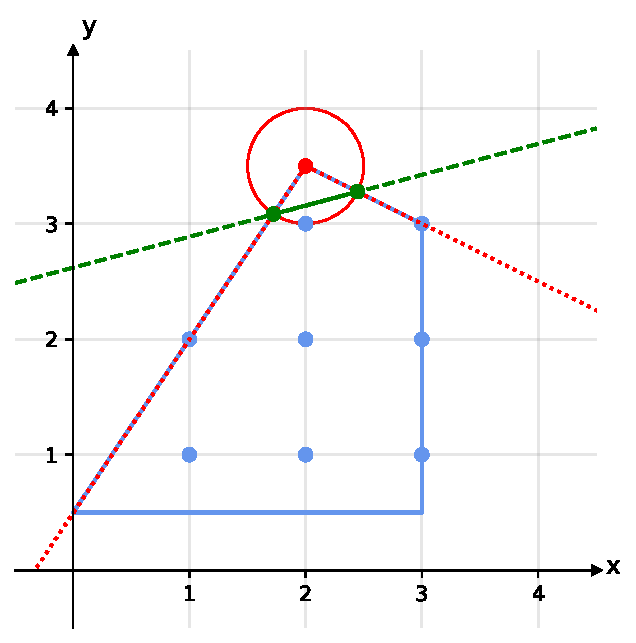
\includegraphics[width=0.6\textwidth]{Images/intersection_cut.pdf}
    \caption{Diagram of intersection cut for \cref{problem:mip_example}}
    \label{fig:intersection_cut}
    \subcaption*{
        The feasible points of the MIP are the integer points respecting the polyhedral constraints (blue points). The set of feasible solutions to the relaxed LP is are all the points in the interior or on the boundary of the polytope (blue line segments). The optimal solution $\bold{ \tilde x}$ to the relaxed LP is the point in the feasible region with the biggest $y$-value (red point). A possible $S$-free set $C$ is a disk with center $\bold{\tilde x}$ and the radius being the distance between $\bold{\tilde x}$ and the closest integer (red circle). The conic relaxation are the extreme rays generated by $\bold{\tilde x}$ which correspond to the two active constraints at $\bold{\tilde x}$ (is indicated by the dotted, red line). The intersection of the conic relaxation and $C$ are the two points in green. The intersection cut is constructed with the line going through the intersecting points (dashed line in green). The area above the green line will be cut off and $\bold{\tilde x}$ is no longer a feasible solution.}
\end{figure} 

The conic relaxation at $\bold{\tilde x}$ is a pointed cone with extreme point $\bold{\tilde x}$ and can be written as: 
\begin{equation} \label{Eq:conic_relaxation}
    P' = \{ \bold{\tilde x} + \sum_{j=1}^n \lambda_j \bold r^j : \boldsymbol \lambda \geq 0 \}
\end{equation}
or as:
\begin{equation} \label{Eq:conic_relaxation_polyhedral}
    P' = \{\bold x|\bold{\tilde Ax} \leq \bold{\tilde b}\}
\end{equation} 
%\unsure[inline]{confusing to have two x?}
where $\bold r^j$ are the extreme rays, $\bold{\tilde A}$ is an invertible $n\times n$ submatrix of $ \bold A$ such that the rows are linearly independent and are a basis for $\bold{\tilde x}$ \cite{bienstock_outer_product_free_sets}. 
% If the original problem is brought in the form $ \bold Ax \leq b$, the bounds on $x$ are included in $ \bold A$ and therefore $m \geq n$. 
A basis for $\bold{\tilde x}$ are the nonbasic constraints at $\bold{\tilde x}$.
If a constraint is nonbasic, the corresponding slack variable of the standard form is nonbasic and therefore 0. This implies that the constraint is active. 

Going back to \cref{problem:mip_example}, the polyhedral presentation of the conic relaxation at $(2, 3.5)$ is:
\begin{equation*}
    P' =     
    \left\{ (x,y) \Bigg|
        \left[ \begin{array}{cc}
            -1.5 & 1 \\
            0.5 & 1
        \end{array}\right]
        \left[ \begin{array}{c}
            x \\ y
        \end{array} \right] \leq
        \left[ \begin{array}{c}
            0.5 \\ 4.5
        \end{array} \right] 
    \right\}
\end{equation*}

The inverse of $\bold{\tilde A}$ is 
\begin{equation*}
    \bold{\tilde A}^{-1} =     
        \left[ \begin{array}{cc}
            -0.5 & 0.5 \\
            0.25 & 0.75
        \end{array}\right]
\end{equation*}
and we get the extreme rays $r_1 = (0.5 -2.5)$ and $r_2= (-0.5, -0.75)$.

After deriving the conic relaxation, we have $\bold{\tilde x} = \bold{\tilde A}^{-1} \bold{\tilde b}$ and $\bold r^j= - \bold{\tilde A}^{-1}_{*,j}$ \cite{bienstock_outer_product_free_sets}. For each extreme ray $\bold r^j$ there either exists an intersection with the boundary of $C$ in which case $\lambda^*_j > 0$ is the step length or the extreme ray is contained in $C$ and $\lambda^*_j= \infty$.
The \textit{intersection cut} is defined as \cite{bienstock_outer_product_free_sets}:
\begin{equation} \label{Eq:interscetion_cut}
    \sum_{i=1}^n (\bold{\tilde a}_{i,*} \bold x - \tilde b_i)/ \lambda_i^* \leq -1
\end{equation}
\quad where $\bold{\tilde a}_{i,*}$ denotes the $i$-th row of basic constraints $\bold{\tilde A}$.

% \unsure[inline]{do we need transpose here? \\MB: depends how you define your notation. It would make more sense to define the selected column as a column vector and use the transpose \\ matches outer-product-free set paper}
\newpage
If we reformulate \cref{Eq:interscetion_cut}, we see that it matches the definition of a cut in \cref{Eq:cuts} \cite{bienstock_outer_product_free_sets}:
\begin{align}
    \sum_{i=1}^n (\bold{\tilde a}_{i,*} \bold x - \tilde b_i)/ \lambda_i^* &\leq -1 \\
    \sum_{i=1}^n ((1/ \lambda_i^*) \bold{\tilde a}_{i,*} \bold x - (1/ \lambda_i^*)\tilde b_i) &\leq -1 \\ 
    \sum_{i=1}^n (1/ \lambda_i^*) \bold{\tilde a}_{i,*} \bold x - \sum_{i=1}^n  (1/ \lambda_i^*)\tilde b_i &\leq -1 \\
    \sum_{i=1}^n (1/ \lambda_i^*) \bold{\tilde a}_{i,*} \bold x & \leq -1 + \sum_{i=1}^n  (1/ \lambda_i^*)\tilde b_i
\end{align}
\begin{equation*}
    \alpha_0 = -1 + \sum_{i=1}^n  (1/ \lambda_i^*)\tilde b_i \quad \quad \alpha_j = \sum_{i=1}^n (1/ \lambda_i^*) \bold{\tilde a}_{i,j} \bold x
\end{equation*}

\todo[inline]{explain why x is cut off}
\todo[inline]{update: basis defining x and basis for P}

% \unsure[inline]{does opt sense matter?\\MB: no it doesn't, intersection cuts don't cut off the objective}
% \todo[inline]{different cut formulations}
% \todo[inline]{use bar or tilde in intersection cuts? tilde already used for combinatorial benders}

\newpage
\thispagestyle{plain}
\section{Metabolic Networks} \label{section:metabolic_networks}
\todo[inline]{brief introduction, shorten intro section, refer to book}
\unsure[inline]{index of v and G differ as they do not have the same length}
\todo[inline]{textsf for problems?}
% \begin{itemize}
%     \item chemical interactions between many of these components are now known and this knowledge gives rise to reconstructed biochemical reaction networks on a genome-scale that underlie various cellular functions
%     \item focus of systems biology on the nature of the links that connect them and on the functional states of the biochemical networks that result from the collection of all such links
%     \item Completing the relationship between all the chemical components of a cell, with their genetic bases, and its physiological functions is the promise of (molecular) systems biology
%     \item genotype: collection of all the genes and the particular
%     version of them found in a genome of an individual organism
%     \item phenotype: form and function of an organism
%     \item possible, in principle, to identify all the gene products
%     that make up an organism
%     \item reconstruct, on a genome-scale, metabolic networks for a
%     target organism in a biochemically detailed fashion ->  can be converted into a mathematical format yielding mechanistic genotype–phenotype relationships for microbial metabolism
%     \item BiGG models represent the reconciliation of the known biochemical properties of the gene products expressed in an organism
%     \item genome-scale models enable the computation of phenotypic traits based on the genetic composition of the target organism
%     \item Cellular functions rely on the coordinated action of the multiple gene products.
% \end{itemize}

% Understanding which chemical reactions take place in an organism, known as \textit{metabolism},  helps to understand cellular behaviour and cellular regulation. Metabolic analysis is important for drug discovery \todo[inline]{Mo: bioprocess optimization, strstrain design, etc.}, as the cellular function often is affected in a disease \cite{fba_applications_and_challenges}.

\textit{Computational systems biology} studies biological systems and biological networks by building and analysing mathematical models that approximate their behaviour \cite{intro_computational_systems_biology}. In this thesis we focus on models at the cellular level.
Instead of looking at the function of all molecules in a cell individually, as in molecular biology, systems biology studies the entire system and especially the links between the different cellular components \cite{palsson_systems_biology}. 
Looking at the system as a whole leads to a different understanding of the cell, as the behaviour of the cell depends on the interaction of the different components and cannot be explained by only studying the function of components individually \cite{intro_computational_systems_biology}.\\
In many cells, the chemical reactions that take place in an organism, known as \textit{metabolism}, determine the central function of the cell \cite{intro_computational_systems_biology}. Understanding the metabolism is therefore necessary in order to understand the cellular behaviour. 
% \todo[inline]{s the central function of a vast majority of cells; therefore, modelling metabolic networks can provide deep insights both into the behaviour of individual organisms \cite{intro_computational_systems_biology}}
% When studying a single cell, we are interested in the internal metabolite concentration, which depends on internal metabolites and reactions \todo[inline]{strange sentence}. 
\textit{Metabolites} are small molecules that are involved in metabolic reactions \cite{intro_computational_systems_biology}. We differentiate between \textit{internal reactions}, involving only internal metabolites, and \textit{exchange reactions}%\todo[inline]{Mo: explain why pseudo reactions}
. Exchange reactions are pseudo reactions representing the transport of metabolites, where either nutrition is taken up or a product is discarded by the cell \cite{fba_applications_and_challenges} \unsure[inline]{is this true in general or just for COBRA models?}. 
In a reaction, a set of metabolites called \textit{reactants} are converted into a different set of metabolites called \textit{products}. The \textit{stoichiometry} is the relative number of metabolites in a reaction. $Enzymes$ are important for the cell metabolism as they \textit{catalyze} reactions, which means that they accelerate reactions without being consumed by it.\\
Graphs can be used to model and understand cellular behaviour \cite{intro_computational_systems_biology}.
In a \textit{metabolic network}, the nodes are metabolites %, called \textit{metabolites}
and the edges represent reactions. 
A \acfi{gem} or \textit{enzyme constrained metabolic model} is a graph that contains all known metabolic information of a biological system such as reactions, metabolites and enzymes \cite{GEMs}.\\ 
The information required to build a GEM comes from a \textit{genome-scale reconstruction}, which is the process of identifying the genome of the organism including different components such as the stoichiometry, reaction direction and the corresponding catalyzing enzymes \cite{fba_applications_and_challenges} \unsure[inline]{about sentence}. 
Depending on the data and assumptions integrated in a model, a different accuracy is achieved, and different questions can be answered \cite{fba_applications_and_challenges}. 
% If one is interested in the dynamics of a system, for example how the metabolite concentration in a cell changes over time, a dynamic model is required. Dynamic models are usually based on differential equations and a large amount of model parameters is required to capture the complexity of a system \cite{intro_computational_systems_biology}.

In this thesis, we focus on constraint-based approaches, also known as \acfi{cobra}. A constraint excludes biologically unrealistic behavior, such as violating the laws of thermodynamics or the conservation of mass \cite{intro_computational_systems_biology}.
With constraint-based methods, one can predict the 
% or \textit{flux distribution} or \textit{reaction rate} %\unsure[inline]{correct?} 
rate of each reaction in the metabolic network \cite{intro_computational_systems_biology}.
% \todo[inline]{quick note on thermodynamics}
The mathematical representation of a metabolic network is described in \cref{section:mathematical_representation}.
The COBRA models relevant for this thesis are presented in \cref{section:optimization_gems}.

\subsection{Mathematical Representation} \label{section:mathematical_representation}
A \textit{hypergraph} $\mathscr{H}$ is defined by its set of vertices $\mathscr{V}$ and set of hyperedges $\mathscr{E}$. A hyperedge is a pair $E_i= (H_i,T_i)$ of disjoint subsets of $\mathscr{V}$, where $H_i$ denotes the vertices in the \textit{head} and $T_i$ the vertices in the \textit{tail}. A path is a sequence of vertices and hyperedges $P_{v_i,v_{q+1}} = (v_i, E_i, ..., E_{j-1}, v_j, E_{j}, ..., E_q, v_{q+1})$ where $v_i \in T_i$, $v_{q+1} \in H_q$ and $v_j \in T_j \cap H_{j-1}$ for all $j = 2,...,q$. A path is a cycle if $v_{q+1}$ is in the tail of $E_i$ \cite{gallo_directed_1993}.\\ %\unsure[inline]{add visualization?} 
A metabolic network $\mathcal{N}$ can be modeled as a hypergraph and is represented by the tuple ($\mathcal{M}, \mathcal{R}, \bold S, \bold l, \bold u$), where $\mathcal M$ is the set of internal metabolites and $\mathcal{R}$ is the set of reactions. The \textit{stoichiometric matrix} $\bold S \in \mathbb{R}^{m\times n}$ captures the entire network, where $m$ is the number of internal metabolites and $n$ is the number of reactions, including internal reactions $\mathcal{I}$ and exchange reactions $\mathcal{E}$. Usually, the number of metabolites is much smaller than the number of reactions \cite{intro_computational_systems_biology}. 
The columns of $\bold S$ correspond to the reactions in the network and the entries are the stoichiometric coefficients for each reaction and capture the mass balance for each metabolite. A negative coefficient indicates that a metabolite is consumed, called \textit{reactant} and is in the tail of the hyperedge. Vice versa, if the coefficient is positive, the metabolite is produced, called \textit{product}, and belongs to the head of the hyperedge.\\
\cref{fig:simple_model} shows a simplified metabolic network with three exchange reactions $\{r_1, r_4, r_8\}$ and five internal reactions $\{r_2, r_3, r_5, r_6, r_7\}$. The set of internal metabolites is $\{A, B, C, D, E, F\}$. The set of reversible reactions is $\{r_5, r_6, r_3\}$ and the set of irreversible reactions $\{r_1, r_2, r_4, r_7, r_8\}$. All irreversible reactions have to be greater or equal to zero. The metabolic network contains the cycle $(A, r_2, E, r_6, D, r_5, A)$.

\begin{figure}[h!]
    \centering
    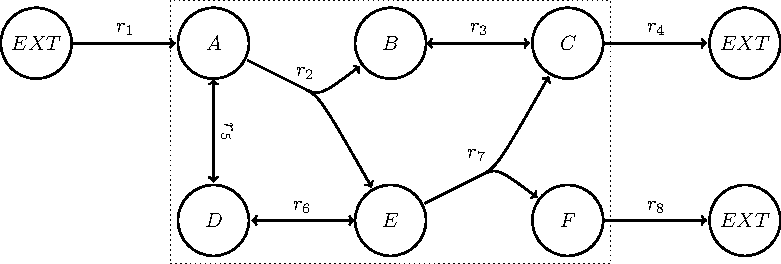
\includegraphics[width=0.8\textwidth]{Images/tikz_graphs_model_with_hyperarcs.pdf}
    \caption{Simplified metabolic network}
    \label{fig:simple_model}
\end{figure}

The corresponding stoichiometric matrix $\bold S$ is:
\begin{equation*}
    \bold S =
    \left[\begin{array}{cccccccc}
        1 & -1 & 0 & 0 & -1 & 0 & 0 & 0\\
        0 & 1 & -1 & 0 & 0 & 0 & 0 & 0\\
        0 & 0 & 1 & -1 & 0 & 0 & 1 & 0\\
        0 & 0 & 0 & 0 & 1 & -1 & 0 & 0\\
        0 & 1 & 0 & 0 & 0 & 1 & -1 & 0\\
        0 & 0 & 0 & 0 & 0 & 0 & 1 & -1\\    
    \end{array}\right]        
\end{equation*}

$\bold S$ is a $6 \times 8$ matrix, where the rows correspond to the internal metabolites in alphabetical order, and the columns denote the reactions $r_i$ in increasing order. In the exchange reaction $r_1$, $A$ is produced, and therefore the corresponding column has a positive entry for $A$. In the internal reaction $v_2$, the consumption of $A$ is captured by a $-1$ and the production of $B$ and $E$ are denoted by a 1 for each metabolite. In this example the quantities for the metabolites are either 0, 1 or -1 in all reactions. In more realistic metabolic models, the stoichiometric coefficients are still integer, but typically vary.
% \unsure[inline]{write bounds explicitly?}

The matrix $\bold S_\mathcal{I}$ is the submatrix of $\bold S$ that contains the columns of internal reactions only. 
The stoichiometric matrix $\bold S$ relates the flux\footnote{\textit{Flux}, \textit{reaction rate} and \textit{flux distribution} are used interchangeably throughout the thesis.} vector $\bold v$ to the change in metabolite concentration $\bold x$: $\frac{d \bold x}{dt} = \bold S \bold v$ \cite{noor_removing_2018}. The vector of flux distributions indicates the units of flow through all reactions. The vectors $\bold l$ and $\bold u$ capture the lower and upper bounds of the flux for all reactions. If the direction of a reaction is forced in one direction by the bounds, the reaction is said to be \textit{irreversible}. Otherwise, it is \textit{reversible}.
The metabolic fluxes are given in units of $\frac{\text{mmol}}{\text{gDW} \times \text{h}}$, which denotes the flux of a metabolite normalized to the biomass of the cell.
%amount of metabolites per hour. 
%which is the concentration per gram dry weight and hourich is the concentration per gram dry weight and hour

\subsection{Optimization for Metabolic Networks} \label{section:optimization_gems}
% \todo[inline]{start with PDE (metabolites are variables) and cobra (fluxes are variables)}
% \todo[inline]{define flux with v = ... ODE paramaters => parameters drop in optimization approach}
% Once a mathematical representation of a model is available, one question is which reaction rates are possible and likely to occur in an organism. 
In dynamic modelling, the dynamics of metabolite concentration are expressed by kinetic laws and kinetic parameters \cite{intro_computational_systems_biology}: 
\begin{equation} \label{Eq:dynamic_model}
    \frac{dx_i}{dt} = f_i(x_1, x_2, ..., x_n; \Theta)
\end{equation}
\quad where $\Theta$ is the set of kinetic parameters and $f_i$ models how the concentration of $x_i$ changes depending on the concentration of the other metabolites. Such a dynamic model requires a lot of computational data in order to predict the metabolite concentration $\bold x$.
% \todo[inline]{dynamic modelling: observe dynamics of a system in terms of the changes in levels of metabolites/genes/proteins \\ require species and interactions -> for each interaction in the model, the right kind of kinetics must be chosen \cite{intro_computational_systems_biology}}

In constraint-based reconstruction and analysis (COBRA) methods, dynamic metabolic networks are modeled at \textit{steady-state}: 
\begin{equation*}
    \frac{d \bold x}{dt} = \bold S \bold v= \bold 0 
\end{equation*} 
\quad where $\bold v \in \mathbb{R}^n$ is the vector of flux distributions, and the stoichiometric matrix $\bold S \in \mathbb{R}^{m \times n}$ captures the topology of the metabolic network. In COBRA methods, the set of possible flux distributions is analysed mathematically, whereas in dynamic modelling, the metabolite concentration is predicted. With COBRA methods one can predict the flux distribution under different environmental conditions and under changes in the environment \cite{intro_computational_systems_biology}.
% \todo[inline]{Constraint-based modelling is focussed on metabolic networks and is most useful to predict the growth rate of a cell, under specific environmental conditions, such as given glucose uptake rate, or following perturbations, such as the knock-out of certain genes from an organism.}
% \todo[inline]{m < r in real metabolic networks. This is because the same metabolites mix and match in different reactions; further, many sink reactions that represent the exchange of intracellular metabolites are always present in the model. Thus, we commonly are confronted with a situation where the number of unknowns is much higher than the number of equations, i.e. the system of linear equations is under-determined. \cite{intro_computational_systems_biology}}
\\
Apart from the steady-state assumption, COBRA methods use context-specific constraints such as \textit{reaction flux bounds} and \textit{mass conservation}. % and the \textit{steady-state assumption} \cite{cobrapy}. 
Mass balance is captured in the stoichiometric matrix $\bold S$. 
%a balance of the produced and consumed metabolite concentration. 
As metabolic reactions take place fast compared to other reactions, such as cell division, the steady-state assumption is biologically plausible \cite{enumerate_extreme_rays}. Compared to the dynamic modeling in \cref{Eq:dynamic_model}, COBRA methods require much less experimental data \cite{intro_computational_systems_biology}.\todo[inline]{reduntant with info in previous paragraph} \todo[inline]{check with optimization section, mention dimension}

% As the number of metabolites $m$ is smaller than the number of reactions $n$, the resulting system of linear equations is underdetermined \cite{intro_computational_systems_biology} 
\textit{Extreme pathways} are a set of vectors that satisfy the model constraints, such that any feasible flux can be written as a convex combination of extreme pathways \cite{price_extreme_2002}.
% The steady-state assumption defines a polyhedral feasible region. The extreme points of the polyhedron are called \textit{extreme pathways}.
There are three types of extreme pathways: \textit{primary systemic pathways} (Type \rom{1}), \textit{futile cycles} (Type \rom{2}) and \textit{internal cycles} (Type \rom{3}). \cref{fig:extreme_pathways} shows the difference between the extreme pathways.
Primary systemic pathways are pathways where exchange reactions are used%\unsure[inline]{should it be two?}
\cite{noor_removing_2018}. These pathways are thermodynamically feasible and are desirable steady-state flux solutions (see \cref{section:ll_fba}). 
For most COBRA methods, the goal is to compute a Type \rom{1} pathway and forbidding Type \rom{2} and Type \rom{3} pathways.\\
In order to understand the difference between Type \rom{2} and Type \rom{3} pathways, we have to introduce \textit{currency exchange reactions}. Currency exchange reactions are a subset of internal reactions, where the currency within the cell is changed \cite{noor_removing_2018}. For example, a reaction, where ATP is generated from ADP, transfers energy and is a Type \rom{2} pathway.\\
Internal cycles are pathways where none of the exchange reactions and none of the currency exchange reactions are used and are thermodynamically infeasible. 
%and are not wanted as steady-state flux solutions
%between different sub-networks in the cell is exchanged. 
Futile cycles are pathways where none of the exchange reactions is used, but at least one currency exchange reaction is used \cite{noor_removing_2018}. \textit{Energy reducing cycles} are futile cycles that are biologically feasible and should be allowed solutions, whereas \textit{energy generating cycles} (EGCs) are futile cycles that are not wanted in a solution \cite{noor_removing_2018}. EGCs are problematic as they can lead to solutions that have a better objective value than when restricting the use of EGCs. One possibility to prevent EGCs is to force the directionality of the reaction. 

\begin{figure}[h!]
    \centering
    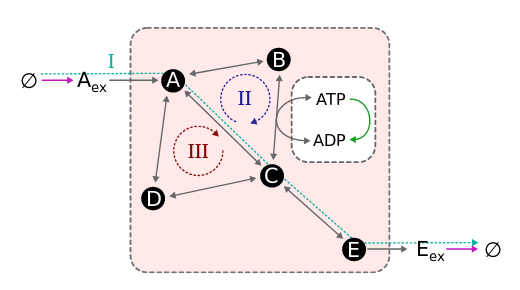
\includegraphics[width=0.6\textwidth]{Images/extreme_pathways.png}
    \caption{Types of extreme pathways}
    \label{fig:extreme_pathways}
    \subcaption*{The figure is taken from \cite{noor_removing_2018}.Primary systemic pathways (Type \rom{1}) are biologically realistic, whereas internal cycles (Type \rom{3}) are not thermodynamically feasible. Futile cycles (Type \rom{2}) can either generate energy or reduce energy. Energy generating cycles are thermodynamically infeasible, whereas energy consuming cycles are realistic.}
\end{figure}
% \unsure[inline]{Mo: all internal cycles are bad}

The feasible region of a COBRA model usually contains multiple solutions. We are interested in flux distributions that optimize a biological objective. A commonly used objective function is the maximization of growth. Growth can be incorporated into the stoichiometric matrix $\bold S$ by adding an extra column where the coefficients indicate the contribution to growth \cite{FBA}. For an overview of biological objectives, see \cite{palsson_systems_biology}.

Depending on the constraints and the objective, we obtain a different COBRA variant. Each corresponds to an optimization problem which can be solved with methods described in \cref{section:optimization}. Several COBRA methods relevant for this thesis are explained below.

\subsubsection{Flux Balance Analysis} \label{section:fba}
The most basic COBRA method is \acfi{fba}. An optimal solution $\bold v^*$ to an \textsf{FBA} model, is a flux distribution maximizing a biological linear objective which respects the steady-state assumption and bound constraints.

\begin{maxi!}
  {\scriptstyle \bold v}{\bold c^\intercal \bold v}{\text{\textbf{FBA}} \label[problem]{problem:fba}}{}
    \addConstraint{\bold S \bold v= \bold 0} \label[constraint]{constraint:fba_b}
    \addConstraint{\bold l \leq \bold v \leq \bold u}
\end{maxi!}
\myproblems{\textsf{FBA} - \cref{problem:fba}}

where $\bold c \in \mathbb{R}^n$ determines the linear objective function of the FBA. The structure of the network is captured in the stoichiometric matrix $\bold S$. The fluxes $\bold v \in \mathbb{R}^n$ are bounded by $\bold l, \bold u \in \mathbb{R}^n$. \cref{constraint:fba_b} ensures the steady-state of the metabolite concentration. We are dealing with a linear program which can be solved efficiently (see \cref{section:Linear Programming}).

As an example, let us consider the metabolic network in \cref{fig:loop}. We have three internal metabolites $A,B,C$, two irreversible exchange reactions $r_1, r_5$ and three reversible internal reactions $r_2, r_3, r_4$. The stoichiometric matrix is: 

\begin{equation} \label{Eq:S_loop}
    \bold S =
    \left[\begin{array}{ccccc}
        1 & -1 & 0 & -1 & 0 \\
        0 & 1 & -1 & 0 & 0 \\
        0 & 0 & 1 & 1 & -1 \\
    \end{array}\right]        
\end{equation}

\quad and we assume the following bounds on the fluxes: 
\begin{equation} \label{Eq:bounds_loop}
    \bold l = (0,-30,-30,-30,0) \quad \bold u = (10,30,30,30,10)
\end{equation}

\begin{figure}[h!]
    \centering
    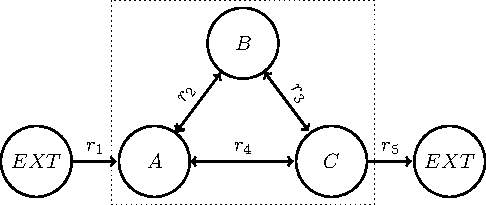
\includegraphics[width=0.6\textwidth]{Images/tikz_graphs_one_loop.pdf}
    \caption{Simple model with internal loop}
    \label{fig:loop}
\end{figure}

If we maximize the flux through the internal reactions, that is $\bold c = (0,1,1,1,0)$, an optimal solution is $\bold v^* = (10, 30, 30, -20, 10)$. The solution contains an internal loop, as there is a flux of 20 going through each of the internal reactions, as seen in \cref{fig:loop_solutions}.

\begin{figure}[H]
    \centering
    \label{fig:loop_solutions}
    \begin{subfigure}{0.5\textwidth}
    \centering
        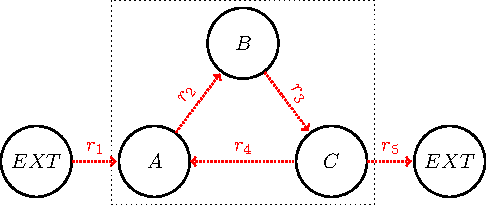
\includegraphics[width=0.99\linewidth]{Images/tikz_graphs_one_loop_fba.pdf}
        \caption{}
    \end{subfigure}%
    \begin{subfigure}{0.5\textwidth}
    \centering
        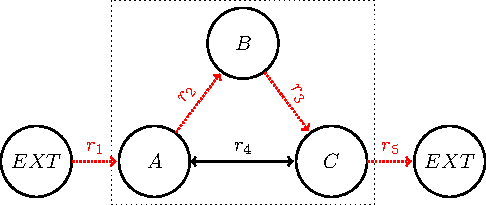
\includegraphics[width=0.99\linewidth]{Images/tikz_graphs_one_loop_ll_fba.pdf}
        \caption{}
    \end{subfigure}
    \caption{Used reactions in the \textsf{FBA} solution (a) which contains an internal cycle, and used reactions in the \textsf{ll-FBA} solution (b).}
\end{figure}

A solution to \textsf{FBA} can be a convex combination of primary systematic pathways, futile cycles and internal cycles. To prevent biologically implausible futile cycles, the directionality is restricted with the bound constraints \cref{problem:fba} (c). Internal cycles are biologically not realistic, but are part of the solution space, posing a major drawback to \textsf{FBA} solutions. 

% \subsubsection{Parsimonous FBA}
% \todo[inline]{add mathematical model}
% \todo[inline]{link to CycleFreeFlux}

\subsubsection{CycleFreeFlux} \label{section:molecular_networks_cyclefreeflux}
Suppose we are given a solution $\bold v^{FBA}$ to an \textsf{FBA} problem (\cref{problem:fba}). 
The following linear program, known as \acfi{cff}, returns a solution $\bold v$ that is structurally consistent with $\bold v^{FBA}$ and with the minimum sum of reaction rates such that the objective values are identical \cite{desouki_cyclefreeflux_2015-1}. 

\begin{mini!}
    {\scriptstyle \bold v}{\sum_i |v_i| = \sum_{i: v_i^{FBA} > 0} v_i - \sum_{i: v_i^{FBA} < 0} v_i}{\text{\textbf{CFF}} \label[problem]{problem:CycleFreeFlux}}{} 
    \addConstraint{\bold S\bold v= \bold 0} \label[constraint]{constraint:CFF_1}
    \addConstraint{{\bold c^\intercal \bold v} = {\bold c^\intercal \bold v}^{FBA}} \label[constraint]{constraint:CFF_2}
    \addConstraint{0 \leq v_i \leq v_i^{FBA} \quad \text{for $i$ with $v_i^{FBA} \geq 0$}} \label[constraint]{constraint:CFF_3}
    \addConstraint{v_i^{FBA} \leq v_i \leq 0 \quad \text{for $i$ with $v_i^{FBA} < 0$}} \label[constraint]{constraint:CFF_4}
    \addConstraint{v_i = v_i^{FBA} \quad \forall i \in \mathcal{E}} \label[constraint]{constraint:CFF_5}
\end{mini!}
\myproblems{\textsf{CFF} - \cref{problem:CycleFreeFlux}}
Beside the steady-state assumption in \cref{constraint:CFF_1}, the reaction direction has to match the direction in $\bold v^{FBA}$ or become zero, enforced by \cref{constraint:CFF_3} and \cref{constraint:CFF_2}. In addition, the reaction rates of the exchange reactions $\mathcal{E}$ remain unchanged (\cref{constraint:CFF_5}).
\cref{constraint:CFF_2} ensures that the objective value of $\bold v$ matches the objective value of $\bold v^{FBA}$. The objective function can be rewritten by replacing the absolute function by the sum of positive reaction rates minus the sum of negative reaction rates, as the sign of reaction rates is known from $\bold v^{FBA}$. As \cref{problem:CycleFreeFlux} is a linear program, it is easy to solve (see \cref{section:solving_lps}). 
If the reactions contained in an internal loop are allowed to be zero, and  if the objective does not depend on a reaction which is contained in an internal loop%, and if the model does not contain energy-generating cycles
, $\bold v$ is thermodynamically feasible \cite{noor_removing_2018}. \unsure[inline]{other cases or disadvantages?}

Let us go back to the \textsf{FBA} example visualized in \cref{fig:loop}. If we apply \textsf{CycleFreeFlux} to the \textsf{FBA} solution $\bold v^{FBA} = (10,30,30,-20,10)$ with $\bold c^\intercal \bold v^{FBA} = 40$, the solution flux 
$\bold v^* = (10,30,30,-20,10)$ still contains an internal loop.

We will see in \cref{section:ll_fba} that formulating a mathematical program such that the resulting flux is in the thermodynamically feasible subspace is $\mathcal{NP}$-hard.

As explained in \cite{desouki_cyclefreeflux_2015-1}, the \textsf{CycleFreeFlux} algorithm can be used to enumerate cycles. For each internal reaction $i$, we solve three LPs. 
We first solve an \textsf{FBA} problem, where we maximize the flux through reaction $i$, whose solution is denoted by $\bold v^{FBA}$. We solve the \textsf{CFF} problem based on $\bold v^{FBA}$, whose solution is denoted by $\bold v^{CFF}$. If $\bold v^{FBA} \neq \bold v^{CFF}$, we know that $\bold v^{FBA}$ contains an internal cycle. We solve another \textsf{CFF} problem based on $\bold v^{FBA}$ with the additional constraint $v_i = v_i^{FBA}$, whose solution is denoted by $\bold v^{(2)}$. The solution $\bold v^{CFF}$ contains one internal cycle, which corresponds to the difference between $\bold v^{(2)} - \bold v^{CFF}$.
\todo[inline]{rename v(2)?}

% \unsure[inline]{how to present paper? Mention complexity of ll-FBA}
% \todo[inline]{mention FVA; FVA possible with cyclefreeflux; mention parsimonous FBA}
% \todo[inline]{compare to parsimonous fba}



% Assuming that no reaction in a loop is maximized in the objective and such reactions are allowed to carry zero flux, 
% solving the LP for a given FBA solution, provides a test for thermodynamic feasibility: $\bold v^{FBA}$ is thermodynamically feasible if $\bold v= \bold v^{FBA}$, where $v$ is the solution to \eqref{problem:CycleFreeFlux}.
% And in that case \eqref{problem:CycleFreeFlux} can be used to enumerate thermodynamically infeasible cycles.  

\subsubsection{Thermodynamic Flux Balance Analysis}
The second law of thermodynamics states that the entropy in a closed system cannot decrease. In a metabolic network, each reaction $i$ is associated with a scalar $\Delta \mu_i$ denoting the \textit{Gibbs free energy change} %\todo[inline]{use Gibbs free energy change everywhere} 
or \textit{potential difference}.
The following has to hold \cite{elimination_infeasible_loops}: 
\begin{equation*}
    \Delta \mu_i = \Delta \mu \degree_i + RT \mathrm{ln} (Q_i)
\end{equation*}

$R$ is the universal gas constant, which relates energy to the amount of substance and temperature, and $T$ the temperature in Kelvin. $Q_i$ is the reaction quotient and denotes the ratio of product concentration to reactant concentration. $\Delta \mu \degree_i$ is the \textit{standard chemical potential}, or \textit{equilibrium potential}, or \textit{standard Gibbs free energy} of reaction $i$.
Instead of using the reaction quotient, we can calculate the concentration of reactants and products in reaction $i$ by using the stoichiometric coefficients $s_{i,*}$ and the metabolite concentration $\bold c$ \cite{noor_removing_2018}:
\begin{equation*}
    \Delta \mu_i = \Delta \mu \degree_i + RT \sum_{i} s_{i,*}^\intercal \mathrm{ln} (\bold c)
    \label{Eq:lawOfThermodynamics}
\end{equation*}
where $\Delta \mu_i$ is the change of Gibbs free energy for reaction $i$. \\
Written in matrix notation, we have:
\begin{equation}
   \boldsymbol{\Delta \mu} = \boldsymbol{\Delta \mu \degree} + RT \bold S^\intercal \mathrm{ln}(\bold c)
\end{equation}

One method that integrates thermodynamic data to get solutions that are thermodynamically feasible is \textit{thermodynamic flux balance analysis} (TFBA). 

\begin{maxi!}
  {\scriptstyle \bold v, \bold a, \bold x, \boldsymbol \mu}{\bold c^\intercal \bold v}{\text{\textbf{TFBA}} \label[problem]{problem:tfba}}{}
    \addConstraint{\bold S \bold v= \bold 0} \label[constraint]{constraint:tfba_1}
    \addConstraint{\bold l \leq \bold v \leq \bold u} \label[constraint]{constraint:tfba_2}
    \addConstraint{0 \leq M \bold a_i-\bold v_i \leq M \quad \forall i \in \mathcal{I}} \label[constraint]{constraint:tfba_3}
    \addConstraint{\epsilon \leq M \bold a_i + \boldsymbol{\Delta \mu_i} \leq M - \epsilon \quad \forall i \in \mathcal{I}} \label[constraint]{constraint:tfba_4}
    \addConstraint{\boldsymbol{\Delta \mu} = \boldsymbol{\Delta \mu \degree} + RT \bold S_{\mathcal{I}}^\intercal \bold x} \label[constraint]{constraint:tfba_5}
    \addConstraint{\mathrm{ln}(\bold b^L) \leq \bold c \leq \mathrm{ln}(\bold b^U)} \label[constraint]{constraint:tfba_6}
    \addConstraint{a_i \in \{0,1\}} \label[constraint]{constraint:tfba_7}
\end{maxi!}
The steady-state constraint (\cref{constraint:tfba_1}), the bound constraints (\cref{constraint:tfba_2}) and the linear objective function correspond to the \textsf{FBA} model (\cref{problem:fba}). \cref{constraint:tfba_3} and \cref{constraint:tfba_4} ensure that the Gibbs free energy is never reduced for any reaction $i$: $v_i = 0 \lor \text{sign}(v_i) = - \text{sign}(\Delta \mu_i)$. $M \in \mathbb{R}$ is a large constant that does not restrict the value of $\bold v$ and $\boldsymbol{\Delta \mu}$. The binary variables $\bold a$ indicate the direction of $\bold v$: $a_i=1$ implies $v_i>0$ and $a_i=0$ implies $v_i<0$. If $a_i=1$, $v_i$ is zero or positive as $-M \leq -v_i \leq M$ holds. $\Delta \mu_i$ is not allowed to be zero so it is bounded by a small value $\epsilon$. In that case, $\Delta \mu_i$ is negative as $\epsilon - M \leq \Delta \mu_i \leq - \epsilon$. If $a_i=0$, $0 \leq -v_i \leq M$ holds and the flux $v_i$ is zero or negative. $\Delta \mu_i$ is positive as $\epsilon \leq \Delta \mu_i \leq M - \epsilon$.
$\bold c$ is the vector of metabolite concentrations which is bounded by $\mathrm{ln}(\bold b^L)$ and $\mathrm{ln}(\bold b^U)$. 
\cite{noor_removing_2018}

A solution to a TFBA model is thermodynamically feasible, however the model requires the standard equilibrium potential for each reaction $\boldsymbol{\Delta \mu \degree}$ which is oftentimes not known. Additionally, the resulting problem is a mixed-integer problem and more difficult to solve than the \textsf{FBA} problem.

\newpage
\subsubsection{Loopless FBA} \label{section:ll_fba}
A simpler method to ensure that a solution does not contain an internal loop, which does not require additional thermodynamic data is \acfi{ll-fba}. 
To respect the second law of thermodynamics, the following inequality for reaction $i$ is required: 
\begin{equation}
    \{v_i = 0\} \lor \{\text{sign}(v_i) = - \text{sign}(\Delta \mu_i)\} 
\end{equation}
\quad which means that if a reaction carries flux, Gibbs free energy decreases \cite{muller_fast_2013}. 
A \textit{loop} is a nonzero flux vector $\boldsymbol \ell$ such that the internal network is at steady-state: $\bold S_{\mathcal{I}} \boldsymbol \ell = \bold 0$ \cite{noor_proof_2012}. As $\ell_i$ and $\Delta \mu_i$ have to be of opposite sign, unless $\ell_i=0$, we know that $\boldsymbol \ell^\intercal \boldsymbol{\Delta \mu} \neq \bold 0$. % sum of negatives and zeros will be negative
However, \textit{flux balance}, or \textit{Kirchhoff's second law}, states that the reaction energies around a circuit have to sum up to zero, and therefore $\boldsymbol \ell$ is not thermodynamically feasible \cite{elimination_infeasible_loops}. 
A flux distribution $\bold v$ contains a loop if there exists a nonzero vector $\boldsymbol \ell$ with $\bold S_{\mathcal{I}} \boldsymbol \ell = \bold 0$ such that: %$\ell_i=0$ or $\ell_i$ and $v_i$ have the same
\begin{equation*}
    \text{sign}(\ell_i) \in \{\text{sign}(v_i),0\} \quad \forall i \in \mathcal{I}
\end{equation*}

For a solution to be thermodynamically feasible, the reaction energies around any flux $\bold v$ have to sum up to zero: $\bold v^\intercal \boldsymbol{\Delta \mu} = 0$, where $\boldsymbol{\Delta \mu}$ is the vector of Gibbs free energy \cite{elimination_infeasible_loops}. As we are interested in internal cycles, it is sufficient to verify that $\bold v_\mathcal{I}^\intercal \boldsymbol{\Delta \mu} =0$, where $\bold v_\mathcal{I}$ is a flux distribution through internal reactions and $\boldsymbol{\Delta \mu}$ are the corresponding changes in Gibbs free energy.
Any steady-state nonzero pathway that just uses internal reactions is a loop: $\bold S_{\mathcal{I}} \bold v_{\mathcal{I}} = \bold 0$ \cite{noor_proof_2012}. The nullspace of $\bold S_{\mathcal{I}}$ is defined as $\mathrm{null}(\bold S_{\mathcal{I}}) := \{\bold x \in \mathbb{R}^{|\mathcal{I}|} : \bold S_{\mathcal{I}} \bold x = \bold 0 \}$. Let $\bold B \in \mathbb{R}^{|\mathcal{I}| \times n}$ be a matrix with columns formed by the set of vectors $\{\bold b_i\}_{i=1}^n$ that form a basis for $\mathrm{null}(\bold S_{\mathcal{I}})$. \todo[inline]{verify dimension}
Any loop $\boldsymbol \ell$ lies in the nullspace of $\bold S_{\mathcal{I}}$ and can thus be written as $\boldsymbol \ell = \bold B ^\intercal \boldsymbol \alpha$ \todo[inline]{transpse needed??}, where coefficients $\alpha_i \in \mathbb{R}$ \cite{elimination_infeasible_loops}. Therefore, the following removes solutions with internal loops: $\bold B^\intercal \boldsymbol{\Delta \mu} = \bold 0$. Adding the loopless constraints to the \textsf{FBA} problem, we obtain the following mathematical program:
\begin{maxi!}
    {\scriptstyle \bold v, \boldsymbol{\Delta \mu}}{\bold c^\intercal \bold v}{\label[problem]{problem:llfba_nullspace}}{}
    \addConstraint{\bold S \bold v= \bold 0} 
    \addConstraint{\bold l \leq \bold v \leq \bold u}
    \addConstraint{\Delta \mu_i v_i < 0 \lor v_i = 0  \quad \forall i \in \mathcal{I}}        
    \addConstraint{\bold B^\intercal \boldsymbol{\Delta \mu} = \bold 0} \label[constraint]{constraint:llfba_nullspace_e}
\end{maxi!}
\enlargethispage{1cm}
\quad where $\bold v \in \mathbb{R}^n$ and $\boldsymbol{\Delta \mu} \in \mathbb{R}^{|\mathcal{I}|}$. For readability, index $i$ corresponds to the pair of $v_i$ and $\Delta \mu_i$, even though $\bold v$ and $\boldsymbol{\Delta \mu}$ are of different length.
\todo[inline]{mention that v and delta mu are of different length, but i is specific index}

We can write \cref{constraint:llfba_nullspace_e} as $\boldsymbol{\Delta \mu} = \bold S ^\intercal \boldsymbol \mu$ \cite{noor_proof_2012, elimination_infeasible_loops, muller_fast_2013}. Let us define the vector of potential differences of the internal reactions as $\boldsymbol{\Delta \mu} = \bold S ^\intercal \boldsymbol \mu$, where $\boldsymbol \mu$ is approximately the chemical potential. Looking only at internal reactions, $\boldsymbol{\Delta \mu}$ is defined as $\boldsymbol{\Delta \mu} = \bold S_\mathcal{I}^\intercal \boldsymbol \mu$.  
Each vector in the rowspace of $\bold S_{\mathcal{I}}$ is orthogonal to each vector in the nullspace of $\mathrm{null}(\bold S_{\mathcal{I}})$ \cite{noor_proof_2012}.
Therefore, $\bold B^\intercal \boldsymbol{\Delta \mu} = \bold 0$. 
\todo[inline]{read paper again}

Rewriting \cref{constraint:llfba_nullspace_e}, we obtain the following mathematical program \cite{muller_fast_2013}:
\begin{maxi!}
    {\scriptstyle \bold v, \boldsymbol{\Delta \mu}, \boldsymbol \mu}{\bold c^\intercal \bold v}{\label[problem]{problem:llfba_original}}{}
    \addConstraint{\bold S \bold v= \bold 0} 
    \addConstraint{\bold l \leq \bold v \leq \bold u}
    \addConstraint{\Delta \mu_i v_i < 0 \lor v_i = 0  \quad \forall i \in \mathcal{I}}        
    \addConstraint{\boldsymbol{\Delta \mu} = \bold S_{\mathcal{I}}^\intercal \boldsymbol \mu} \label[constraint]{constraint:llfba_original_e}
    % \addConstraint{\mu \in \mathbb{R}^m}
    % \addConstraint{\Delta \mu \in \mathbb{R}^n}
    % \addConstraint{v \in \mathbb{R}^n}
    % \addConstraint{\bold S \in \mathbb{R}^{m\times n}}
\end{maxi!}
where $\boldsymbol \mu \in \mathbb{R}^m$ and $\boldsymbol{\Delta \mu} \in \mathbb{R}^{|\mathcal{I}|}$. 
\cref{problem:llfba_original} is $\mathcal{NP}$-hard and much more complicated to solve than \textsf{FBA} \cite{cornelis_metabolic_nodate}. We use $\boldsymbol{\Delta \mu}$ and $\boldsymbol \mu$ due to the biological interpretability, however it is not necessary to define $\boldsymbol{\Delta \mu}$ as it only appears in \cref{constraint:llfba_original_e}.

Constraint (d) in \cref{problem:llfba_original} and \cref{problem:llfba_nullspace} poses a challenge due to the disjunction, the strict equality and the product of decision variables $\boldsymbol{\Delta \mu}$ and $\bold v$. To simplify the model, the disjunction is rewritten and we arrive at the loopless FBA model used in this thesis.

\begin{maxi!}
    {\scriptstyle \bold v, \boldsymbol{\Delta \mu}, \boldsymbol \mu}{\bold c^\intercal \bold v}{\text{\textbf{ll-FBA}} \label[problem]{problem:llfba}}{}
    \addConstraint{\bold S \bold v= \bold 0} \label[constraint]{constraint:llfba_b}
    \addConstraint{\bold l \leq \bold v \leq \bold u} \label[constraint]{constraint:llfba_c}
    \addConstraint{\begin{aligned} &\bigl((v_i \geq 0) \land (\Delta \mu_i \leq - \epsilon) \bigr) \, \, \lor \\ 
    &\bigl((v_i \leq 0) \land (\Delta \mu_i \geq \epsilon) \bigr) \end{aligned} \quad \quad \forall i \in \mathcal{I}} \label[constraint]{constraint:llfba_d}
    \addConstraint{\boldsymbol{\Delta \mu}^\intercal = \boldsymbol \mu^\intercal \bold S_{\mathcal{I}}} \label[constraint]{constraint:llfba_e}
    % \addConstraint{\mu \in \mathbb{R}^m}
    % \addConstraint{\Delta \mu \in \mathbb{R}^n}
    % \addConstraint{v \in \mathbb{R}^n}
    % \addConstraint{\bold S \in \mathbb{R}^{m\times n}}
\end{maxi!}
\myproblems{\textsf{ll-FBA} - \cref{problem:llfba}}
Whereas the value of $\boldsymbol{\Delta \mu}$ in TFBA corresponds to the Gibbs free energy change tested in experiments, in ll-FBA only the $\text{sign}(\boldsymbol{\Delta \mu})$ corresponds to the actual Gibbs free energy change \cite{elimination_infeasible_loops}. 
As the value does not matter, we can scale $\boldsymbol{\Delta \mu}$ by not allowing it to be in the interval $[- \epsilon , \epsilon ]$.
The resulting problem is a disjunctive program with linear constraints in the disjunctions and can be reformulated as a mixed-integer program with indicator or big-M constraints (see \cref{section:solving_dps}). 

% \todo[inline]{explain why this is ok (M.)}
% \todo[inline]{cite proofs, especially complexity proof}

Going back to the previous example with $\bold S$ defined in \cref{Eq:S_loop} and flux bounds defined in \cref{Eq:bounds_loop},  
the loopless flux distribution is $\bold v^* = (10,10,10,0,10)$ with $\bold c^\intercal \bold v^* = 20$ which is shown in \cref{fig:loop_solutions}. 
\todo[inline]{fix reference}

Loopless FBA excludes internal cycles from the solution space. However, energy generating cycles still have to be blocked by restricting the directionality.

\subsubsection{st-FBA}
\textit{Semi-thermodynamic Flux Balance Analysis} (st-FBA) combines the loopless FBA and TFBA approaches \cite{noor_removing_2018}. The loopless FBA formulation is extended by constraining the Gibbs free energy change $\boldsymbol{\Delta \mu}$ of a subset of reactions. Metabolites that carry energy such as ATP and their related compounds such as ADP and AMP are treated as in TFBA. The chemical potential of such a metabolite is limited by bounds known from experiments. Bounding the chemical potential of these energy-carrying currency metabolites excludes energy generating cycles, and it is no longer required to force the direction of certain reactions as in ll-FBA. 
st-FBA is thus a trade off between the $\boldsymbol{\Delta \mu}$ values corresponding to the Gibbs free energy changes which requires experimental data, and the approximation of the Gibbs Free energy changes which only deals with the directionality.
We require more experimental data than for ll-FBA, as we need the bounds of reactions involved in energy reducing cycles. As we add the experimental data just on a small subset of reactions, just a fraction of information needed for TFBA is needed for st-FBA.
% \unsure[inline]{why S not in constraints (30)-(31)?}
% \todo[inline]{why model exists, advantages, disadvantages, compare to ll-FBA and TFBA (M.)}

\subsubsection{Enzyme Constrained Metabolic Models}
In FBA, the optimal reaction rate of a metabolic network is limited by the nutrition uptake. However, the flux depends also on the enzyme abundances catalysing the reactions. Especially modelling physiological responses, such as \textit{overflow metabolism}, requires enzymatic data \cite{improving_phenotype_predictions}. Overflow metabolism refers to the phenomenon that a cell uses fermentation instead of respiration, even though respiration is more energetically efficient \cite{overflow}. There are several hypotheses to explain the metabolic switch from respiration to fermentation. One hypothesis is that overflow metabolism is connected to the enzyme mass. When using fermentation, the cell does not grow as fast as with respiration, but it yields more energy with the same enzyme mass \cite{improving_phenotype_predictions}.  
\textit{GECKO} is one method that integrates enzyme constraints into a genome-scale model. The following section is based on \cite{improving_phenotype_predictions}. 

\newpage
Suppose reaction $j$ is catalysed by enzyme $E_i$. The \textit{turnover number} indicates how efficient an enzyme is. The reaction rate $v_j$ depends on the \textit{enzyme usage} $e_i$ and the turnover number $k_{cat}^{ij}$: 
\begin{equation} \label{Eq:enzyme_mass_balance}
    k_{cat}^{ij} e_i = v_j   
\end{equation}
The turnover number is given in $\frac{1}{\text h}$, the enzyme usage in $\frac{\text{mmol}}{\text{gDW}}$, such that $\bold v$ has the unit of $\frac{\text{mmol}}{\text{gDW} \times \text h}$. 
\cref{Eq:enzyme_mass_balance} is also known as \textit{enzyme mass balance}.
To account for enzyme mass balance in a GEM, matrix $S^{GECKO}$ is constructed by extending the stoichiometric matrix $\bold S$ by three submatrices. 
A row is added for each enzyme $E_i$ and a column for the corresponding enzyme usage $e_i$, with $p$ enzymes. The lower left submatrix contains the enzyme information on the diagonal, that is $-1/k_{cat}^{ij}$. The lower right matrix is the identity matrix. The upper right matrix contains only zeros.
The resulting matrix is of the form:
\begin{equation*}
    S^{GECKO} = \left[\begin{array}{ccc|ccc} 
        s_{1,1} & \text{...} & s_{1,n} & 0 & \text{...} & 0 \\ 
        \vdots & \ddots & \vdots & \vdots & \ddots & \vdots \\
        s_{m,1} & \text{...} & s_{m,n} & 0 & \text{...} & 0 \\
        \hline 
        -1/k_{cat}^{11} & \text{...} & 0 & 1 & \text{...} & 0 \\ 
        \vdots & \ddots & \vdots & \vdots & \ddots & \vdots \\
        0 & \text{...} & -1/k_{cat}^{pn} & 0 & \text{...} & 1
    \end{array}\right] = 
    \left[\begin{array}{cc} 
        \bold S & \bold 0_{m,p} \\
        \text{diag} (-1/k_{cat}^{ij}) & \bold I_p
    \end{array}\right]
\end{equation*}

In addition to the reaction rates $\bold v$, we are interested in the enzyme usage $\bold e$. We obtain the following optimization problem:
\begin{maxi!}
    {\scriptstyle \bold v, \bold e}{\bold c^\intercal \bold v}{\label[problem]{problem:Gecko}}{}
    \addConstraint{S^{GECKO} (\bold v, \bold e)= \bold 0} \label[constraint]{constraint:Gecko_1}
    \addConstraint{\bold l \leq \bold v \leq \bold u} \label[constraint]{constraint:Gecko_2}
    \addConstraint{\bold 0 \leq \bold e \leq [\bold E]} \label[constraint]{constraint:Gecko_3}
\end{maxi!}
\quad where $[\bold E]$ is the vector of intracellular enzyme concentrations.
\todo[inline]{E is vector but capitalised}
The objective function and \cref{constraint:Gecko_2} are also part of the \textsf{FBA} problem.
\cref{constraint:Gecko_1} forces a steady-state of the metabolites and enzyme mass balance. As the upper right matrix contains only zeros, the steady-state constraint $\bold S \bold v= \bold 0$ is preserved.
In addition to bounds on the fluxes, \cref{constraint:Gecko_3} limits the enzyme usage $e_i$, which cannot be negative and has to be below the intracellular enzyme concentration $[E_i]$: 
\begin{equation*}
    0 \leq e_i \leq [E_i]    
\end{equation*}

Together both lower submatrices of $S^{GECKO}$ make up the enzyme mass balance constraints: 
\begin{align*}
    -\frac{1}{k_{cat}^{ij}}v_j + e_i &= 0 \\
    e_i &= \frac{1}{k_{cat}^{ij}} v_j \\
    k_{cat}^{ij} e_i &= v_j
\end{align*}

Depending on the type of enzyme, $S^{GECKO}$ is modified slightly. If different enzymes catalyze the same reaction, they are called \textit{isozymes} and one mass balance constraints for each isozyme is added to the model.

\unsure[inline]{proteins or enzymes in gecko model? compare to methods gecko models}
If the intracellular enzyme concentration is not known, the total enzyme abundance is limited.   
\cref{constraint:Gecko_3} is replaced by:
\begin{equation*}
    \sum_i^p \text{MW}_i e_i \leq P
\end{equation*}
\quad where $\text{MW}_i$ is the molecular weight of enzyme $i$ and $P$ is the total protein content in the cell \cite{improving_phenotype_predictions}.
\clearpage
\section{Methods}
\todo[inline]{differentiate between cycle in network and loop in flux}
\todo[inline]{mention scaling of epsilon; why eps = 1 in computation}
In \cref{section:metabolic_networks}, we have seen how mathematical optimization can be used to predict fluxes $\bold v$ in a cell that optimize a biological objective. In particular ll-FBA (\cref{problem:llfba}) can be used to predict fluxes that do not contain internal loops. However, ll-FBA is difficult to solve due to the constraint that $\Delta \mu_i$ and $v_i$ have to be of opposite sign, unless $v_i=0$, which is modeled by a disjunction. In this thesis, we compare the runtime of the big-M reformulation of ll-FBA to the convex-hull reformulation and to solving the problem by adding cutting planes. 

\todo[inline]{technical setup, github link}
The code is written in \textsf{Julia} 1.9.0. We use \textsf{JuMP} \cite{JuMP} and \textsf{MathOptInterface} \cite{mathoptinterface} to build the mathematical models. The MIP solver used in the experiments is \textsf{SCIP} \cite{SCIP}. The LP solver used is \textsf{HiGHS} \cite{HiGHS}. We use \textsf{COBREXA}\cite{cobrexa} to load the biological model data.

\todo[inline]{rewrite following section, shorten section}
\todo[inline]{present more why you have done what and then link the sections}
% delayed constrained generation for cuts
In \cref{section:feasibility_test}, we explain briefly how we test for a solution whether it does not contain internal loops. 
In \cref{section:llfba_variants}, we see how ll-FBA can be reformulated with indicator constraints, and with big-M constraints.
In \cref{section:blocking_cycles}, we take a solution to the FBA problem (\cref{problem:fba}) which may contain internal loops. Loops are identified and cuts are added to the ll-FBA formulation to exclude solutions that contain a specific loop from the feasible region.
In \cref{section:no_good_cuts}, we solve a relaxed version of ll-FBA, where we solve an FBA, but assign binary variables dependent on the directionality of $\bold v$. If a solution to the relaxed problem is not a feasible solution to the ll-FBA problem, a cut is added to the relaxed problem that cuts off the assignment of binary variables. This procedure is repeated until a solution is found that is a feasible solution to ll-FBA. 
We will see in \cref{section:cb} how to generate stronger cuts than a no-good cut using combinatorial Benders' cuts. The ll-FBA problem is split into a master problem and subproblem and we exploit the duality of the infeasible subproblem to generate cuts that include a subset of binary variables only. 
Another type of cuts are intersection cuts, explained in \cref{section:methods_interscetion_cuts}. The feasible region is split into the polyhedral set $P$, which contains the inequality and equality constraints, and the set $S$, which contains the disjunctions. An S-free set $C$ is defined around a solution $\boldsymbol{\tilde x}$ that lies in $P$ but not in $S$. The intersection cut is the hyperplane going through the intersection of the conic relaxation at $\boldsymbol{\tilde x}$ with $C$. 
In \cref{section:disjunctive_programming}, the ll-FBA problem is written as disjunctive problem, which includes a binary variable for each disjunct. The problem is then solved by using the big-M reformulation and the convex-hull reformulation. In \cref{section:models} we introduce the data that is used for the experiments.

% \todo[inline]{put FBA and ll-FBA in standard form}
% \todo[inline]{explain why indicator constraints can be used in CB}
% \todo[inline]{add pseudo code}

\subsection{Feasibility Test} \label{section:feasibility_test}
For a given flux distribution $\boldsymbol{\tilde{v}}$ and the corresponding directions $\boldsymbol{\tilde{a}}$ the following problem is feasible if it is loopless:
\begin{maxi!}
    {\scriptstyle \boldsymbol{\Delta \mu}, \boldsymbol \mu}{0}{\label[problem]{problem:feasiblityCheck}}{} 
    \addConstraint{-M \leq \Delta \mu_i \leq - \epsilon \quad} {\forall i \in \mathcal{I}: \tilde{a_i} = 1}    
    \addConstraint{\epsilon \leq \Delta \mu_i \leq M \quad} {\forall i \in \mathcal{I}: \tilde{a_i} = 0}        
    \addConstraint{\boldsymbol{\Delta \mu} = \bold S_{\mathcal{I}}^\intercal \boldsymbol \mu}{}
    % \addConstraint{\mu \in \mathbb{R}^m}
    % \addConstraint{\Delta \mu \in \mathbb{R}^n}
    % \addConstraint{v \in \mathbb{R}^n}
    % \addConstraint{S \in \mathbb{R}^{m\times n}}
\end{maxi!} 
\quad where we set the big-M constant to 1000 and $\epsilon$ to 1. 

Note that if $\tilde{v_i} = 0$, the reaction can be removed from the problem by removing the reaction from $\bold S_{\mathcal{I}}$ and without adding variable $\Delta \mu_i$. 
\cref{problem:feasiblityCheck} can also be used to test the looplessness of a solution and a subset of internal reactions by setting the flux of all other reactions to zero.

Going back to the example visualized in \cref{fig:loop} in \cref{section:fba}, for the solution $\boldsymbol{\tilde v} = (10, 30, 30, -20, 10)$ where $\tilde v_2, \tilde v_3, \tilde v_4$ are the fluxes through the internal reactions, and $\boldsymbol{\tilde a} = (1,1,0)$. The solution contains a loop and \cref{problem:feasiblityCheck} is infeasible. 

For the loopless solution $\boldsymbol{\tilde v} = (10, 10, 10, 0, 10)$, we only look at the non-zero internal fluxes $\tilde v_2, \tilde v_3$ and the corresponding directionality is $\boldsymbol{\tilde a} = (1,1)$. \cref{problem:feasiblityCheck} is feasible, and the solution is $\boldsymbol{\Delta \mu}=(-1, -1)$ and $\boldsymbol \mu = (2,1,0)$. 

\subsection{Loopless FBA Formulations} \label{section:llfba_variants}
We can reformulate \cref{problem:llfba} to no longer write the disjunctions explicitly.
The mixed-integer program of flux balance analysis without unbounded internal cycles using indicator constraints \cite{elimination_infeasible_loops}:

\begin{maxi!}
    {\scriptstyle \bold v, \bold a, \boldsymbol{\Delta \mu}, \boldsymbol \mu}{\bold c^\intercal \bold v}{\text{\textbf{ll-FBA (indicator):}} \label[problem]{problem:thermo_fba_indicator}}{}
    \addConstraint{\bold S \bold v=\bold 0} \label[constraint]{constraint:thermo_fba_indicator_b}
    \addConstraint{\bold l \leq \bold v \leq \bold u} \label[constraint]{constraint:thermo_fba_indicator_c}
    \addConstraint{a_i = 1}{\quad \implies \quad v_i \geq 0}{\quad \forall i \in \mathcal{I}} \label[constraint]{constraint:thermo_fba_indicator_d}
    \addConstraint{a_i = 1}{\quad \implies \quad \Delta \mu_i \leq - \epsilon}{\quad \forall i \in \mathcal{I}} \label[constraint]{constraint:thermo_fba_indicator_e}
    \addConstraint{a_i = 0}{\quad \implies \quad v_i \leq 0}{\quad \forall i \in \mathcal{I}} \label[constraint]{constraint:thermo_fba_indicator_f}
    \addConstraint{a_i = 0}{\quad \implies \quad \Delta \mu_i \geq \epsilon}{\quad \forall i \in \mathcal{I}} \label[constraint]{constraint:thermo_fba_indicator_g}
    % \addConstraint{\bold B^\intercal \boldsymbol{\Delta \mu} = \bold 0}
    \addConstraint{\boldsymbol{\Delta \mu} = \bold S_{\mathcal{I}}^\intercal \boldsymbol \mu} \label[constraint]{constraint:thermo_fba_indicator_h}
    % \addConstraint{a \in \{0,1\}^n}
    % \addConstraint{\Delta \mu \in \mathbb{R}^n}
    % \addConstraint{v \in \mathbb{R}^n}
    % \addConstraint{S \in \mathbb{R}^{m\times n}}
\end{maxi!}

The mixed-integer program of flux balance analysis without unbounded internal cycles using big-M constraints \cite{elimination_infeasible_loops}:
%TODO dimension of variables

\begin{maxi!}
    {\scriptstyle \bold v, \bold a, \boldsymbol{\Delta \mu}, \boldsymbol \mu}{\bold c^\intercal \bold v}{\text{\textbf{ll-FBA (big-M):}} \label[problem]{problem:thermo_fba_bigM}}{}
    \addConstraint{\bold S \bold v= \bold 0} 
    \addConstraint{l \leq v \leq u}
    \addConstraint{-Ma_i + \epsilon(1-a_i) \leq \Delta \mu_i \leq - \epsilon a_i + M(1-a_i) \quad \forall i \in \mathcal{I}}        
    \addConstraint{-M(1-a_i) \leq v_i \leq M a_i \quad \forall i \in \mathcal{I}}
    % \addConstraint{\bold B^\intercal \boldsymbol{\Delta \mu} = \bold 0} \label[constraint]{constraint:thermo_fba_bigM_f}
    \addConstraint{\boldsymbol{\Delta \mu} = \bold S_{\mathcal{I}}^\intercal \boldsymbol \mu} \label[constraint]{constraint:thermo_fba_bigM_f}
    % \addConstraint{a \in \{0,1\}^n}
    % \addConstraint{\Delta \mu \in \mathbb{R}^n}
    % \addConstraint{v \in \mathbb{R}^n}
    % \addConstraint{S \in \mathbb{R}^{m\times n}}
\end{maxi!}
The big-M formulation ensures the opposite sign of $v_i$ and $\Delta \mu_i$ if $v_i \neq 0$. If the flux through reaction $i$ is a forward flux, that is $v_i > 0$ and $a_i=1$, it holds that $-M \leq \Delta \mu_i \leq -\epsilon$ and analogously for a backward flux. We set $\epsilon$ to 1, and the big-M constant is the maximal absolute value of the flux bounds $\bold l, \bold u$. \todo[inline]{reference scaling again}
As explained in \cref{section:ll_fba}, \cref{constraint:thermo_fba_indicator_h,constraint:thermo_fba_bigM_f} can be replaced by $\bold B^\intercal \boldsymbol{\Delta \mu} = \bold 0$.

\subsection{Blocking Cycles} \label{section:blocking_cycles}
\todo[inline]{use CycleFreeFlux instead?}
\unsure[inline]{mention CycleFreeFVA here or in bio section}
We take an optimal solution  $\bold v^*$ to \cref{problem:fba}. The metabolic network and the  $\bold v^*$ are transformed such that the hyperarcs are split into simple directed edges. We search for loops in the transformed graph on edges with nonzero flux. Finally, we check whether the loop found in the transformed graph is a thermodynamically infeasible loop in the metabolic network. An internal loop can be removed by adding a constraint to \cref{problem:llfba_original}. 

The hyperarcs represented by $\bold S$ are split up by replacing each hyperarc $E= (H,T)$ by $k$ simple directed edges for every pair in $H \times T$. The transformed matrix is denoted by $\bar{\bold S}$. Assume the flux though hyperarc $E$ is $v^*_E$. $\bar{\bold v}$ has then $n$ entries with $v^*_E$.
For every nonzero reaction in $v^*$, the corresponding reactions of $\bar{\bold S}$ are used to construct a simple directed graph $G$. We use the \textsf{Graph} package to build the graph and \textsf{simplecycles\_iter} %\footnote{\url{https://juliagraphs.org/Graphs.jl/dev/algorithms/cycles/#Graphs.simplecycles_iter}} 
to compute the set of cycles in $G$ \cite{Graphs2021}. We test for a cycle in the transformed network, whether the corresponding reactions in $\bold S$ are thermodynamically feasible (see \cref{section:feasibility_test}).
To block a given cycle, a Boolean expression is added as a constraint ensuring that the $a_i$'s for reactions $i$ in the cycle are assigned differently. 

Suppose we have a solution that contains a loop $\boldsymbol \ell$ %: $\bold S_{\mathcal{I}} \boldsymbol \ell = \bold 0$, 
and let $\bold a$ be the corresponding binary variables indicating the direction of the flux. We can write the assignment of binary variables as Boolean expression: $t_1 \land ... \land t_i \land ... t_{|\mathcal{I}|}$, where $t_i = a_i$ if $a_i=1$ and otherwise $t_i = 1 -a_i$.
To block the cycle, the assignment of the $a_i$'s has to be constrained: 
    $\neg (t_1 \land ... \land t_i \land ... t_{|\mathcal{I}|}) \, = 1$.
Formulating the expression as linear constraint yields:
    $t_1 + ... + t_i + ... t_{|\mathcal{I}|} \geq 1$.
    % # to block cycle: ¬(a1 ∧ a2 ∧ a3) = ¬a1 ∨ ¬a2 ∨ ¬a3 >= 1
    % # ¬a1 = 1 - a1 => 
    % # 1-a1 ∨ 1-a2 ∨ 1-a3 >= 1 
    % # -a1 ∨ -a2 ∨ -a3 >= 1-3 = -2
    % # for backward arc: ¬(¬a1) = a1

A detected cycle can be blocked by a cut in the thermodynamic feasible FBA. The solution will not be impacted, but the run time can be affected. 
% numbers of cycles
% The number of cycles blocked has a strong impact on the run time. There is a significant slow down if the number of cycles is greater than ... 
% shortest cycles
We filter the thermodynamically infeasible cycles in the set of cycles found in the transformed graph. Instead of blocking all detected cycles, we experiment with blocking the smallest cycles, which potentially leads to stronger cuts. 

\todo[inline]{example}

\subsection{No-Good Cuts} \label{section:no_good_cuts}
When using no-good cuts to solve ll-FBA, the solving procedure is divided into first solving the relaxed problem and then checking the feasibility of the solution to the relaxed problem. 
The following relaxed version of \cref{problem:thermo_fba_indicator} is solved, where the loopless constraints are ignored, but the indicator variables $\bold a$ are assigned:
\begin{maxi!}
    {\scriptstyle \bold v, \bold a}{\bold c^\intercal \bold v}{\label[problem]{problem:noGoodCut}}{} 
    \addConstraint{\bold S \bold v= \bold 0} 
    \addConstraint{\bold l \leq \bold v \leq \bold u}
    \addConstraint{a_i = 1}{\quad \implies \quad v_i \geq 0}{\quad \forall i \in \mathcal{I}}      \addConstraint{a_i = 0}{\quad \implies \quad v_i \leq 0}{\quad \forall i \in \mathcal{I}}
\end{maxi!}

The indicator constraints can be linearized by using the big-M method.
If a solution $\bold x^{IP}$ to \cref{problem:noGoodCut} is thermodynamically infeasible, the following constraint is added:

\begin{equation} \label{noGoodCut}
\sum_{i \in \mathcal{I}: x_i^{IP}=1} a_i + \sum_{i \in \mathcal{I}: x_i^{IP}=0} (1-a_i) \leq |\mathcal{I}|-1
\end{equation}

The problem is now solved again and this procedure is repeated until a solution is thermodynamically feasible. 

As an example, let us consider the metabolic network in \cref{fig:two_internal_loops}. We have four internal metabolites $A,B,C, D$, two irreversible exchange reactions $r_1, r_5$, two irreversible internal reactions $ r_6, r_7$ and three reversible internal reactions $r_2, r_3, r_4$. We assume the following bounds on the fluxes: 
\begin{equation*} \label{Eq:bounds_loop}
    \bold l = (0,-10,-10,-20,0,0,0) \quad \bold u = (20,30,30,30,20,10,10)
\end{equation*}
\begin{figure}[h!]
    \caption{simple model with two internal loops}
    \centering
    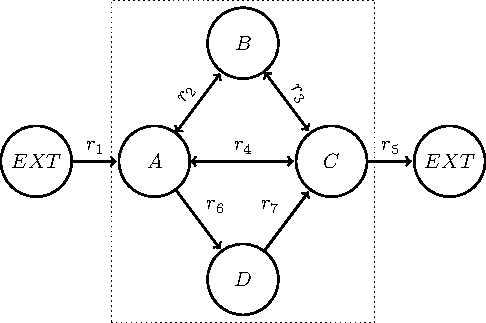
\includegraphics[width=0.8\textwidth]{Images/tikz_graphs_two_loops.pdf}
    \label{fig:two_internal_loops}
\end{figure}
\todo[inline]{show flux in color}
If we maximize the flux through the all reactions, that is $\bold c = \bold 1$, the optimal solution is $\bold v^* = (20, 30, 30, -20, 20, 10, 10)$ and $\bold a = (1,1,0,1,1)$. The solution is not thermodynamically feasible as it contains two internal loops. The corresponding no-good cut is:
\begin{equation*}
    (1-a_3) + \sum_{i \in \{1,2,4,5\}} a_i \leq 5-1
\end{equation*}

\subsection{Combinatorial Benders' Cuts} \label{section:cb}
 When deriving combinatorial Benders' cuts for ll-FBA, the solving procedure is divided into first solving the relaxed problem and then checking the feasibility of the solution to the relaxed problem, similar to the no-good cut derivation. However, instead of forbidding the infeasible solution found to the relaxed problem, we aim at identifying the variables that lead to the thermodynamic infeasibility, and potentially derive stronger cuts.

ll-FBA matches the required problem form \cref{problem:mathematical_program_CB}. We have a linear objective $\bold c^\intercal \bold v$, continuous variables $\bold v$ and $\boldsymbol{\Delta \mu}$, and a set of binary variables $\bold a$. There are linear constraints on the continuous variables \cref{constraint:thermo_fba_indicator_b,constraint:thermo_fba_indicator_c,constraint:thermo_fba_indicator_h}, and no constraints on the binary variables. The continuous variables and the binary variables are only connected by the indicator constraints (\cref{constraint:thermo_fba_indicator_d,constraint:thermo_fba_indicator_e,constraint:thermo_fba_indicator_f,constraint:thermo_fba_indicator_g}), and we can split the MIP into a master and a subproblem.
The master problem (MP) is
% \begin{maxi!}
%     {\scriptstyle \bold v, \bold a}{\bold c^\intercal \bold v}{\label[problem]{problem:masterProblem}}{} 
%     \addConstraint{\bold S \bold v = \bold 0} 
%     \addConstraint{\bold l \leq \bold v \leq \bold u}
%     \addConstraint{a_i = 1}{\quad \implies \quad v_i \geq 0}{\quad \forall i \in \mathcal{I}}      \addConstraint{a_i = 0}{\quad \implies \quad v_i \leq 0}{\quad \forall i \in \mathcal{I}}
% \end{maxi!}
\cref{problem:noGoodCut}
and the subproblem (SP) is the following \textit{parameterised program}:
\begin{maxi!}
    {\scriptstyle \boldsymbol{\mu, \Delta \mu}}{0}{\label[problem]{problem:methods_subProblem}}{} 
    \addConstraint{a_i^{MP} = 1}{\quad \implies \quad \Delta \mu_i \leq - \epsilon}{\quad \forall i \in \mathcal{I}}
    \addConstraint{a_i^{MP} = 0}{\quad \implies \quad \Delta \mu_i \geq \epsilon}{\quad \forall i \in \mathcal{I}} \label[constraint]{constraint:subProblem_c}
    % \addConstraint{c^\intercal v \geq \mathcal{UB} + \epsilon}
    \addConstraint{\boldsymbol{\Delta \mu} = \bold S_{\mathcal{I}}^\intercal \boldsymbol \mu} \label[constraint]{constraint:subProblem_d}
\end{maxi!}

\quad where $\bold a^{MP}$ are the values of a solution to the master problem. If the subproblem is infeasible, we compute a corresponding minimal infeasible subsystem (MIS) $\mathcal{C}$. The minimal infeasible subsystem contains a minimal number of constraint indices that make the subproblem infeasible.
The following combinatorial Benders' (CB) cut is added to the master problem if the subproblem is infeasible:
\begin{equation*}
\sum_{i \in \mathcal{C}: a_i^{MP}=0} a_i + \sum_{i \in \mathcal{C}: a_i^{MP}=1} (1-a_i) \geq 1
\end{equation*}
Note that if $\mathcal{C}$ contains all internal reactions $\mathcal{I}$, the CB cut corresponds to a no-good cut (\cref{noGoodCut}).

The pseudocode for the combinatorial Benders' cut procedure is shown in \cref{alg:CB}. In \textsf{build\_master\_problem}, the MP is built, which is the FBA problem with binary variables $\bold a$ that are linked to the directionality of $\bold v$. The relation between the flux variables $\bold v$ and the binary variables $\bold a$ can be expressed by indicator constraints as in \cref{problem:noGoodCut}, by big-M constraints, or by indicator constraints and big-M constraints simultaneously. The big-M constant corresponds to the maximal absolute value of lower bounds $\bold l$ and upper bounds $\bold u$.
The set of minimal infeasible subsystems is computed in \textsf{compute\_mis}, which identifies at most $m$ subsystems. The MIS search is explained in detail in \cref{section:methods_mis}. The dual problem of the infeasible subproblem is built with the \textsf{Dualization} package \cite{dualization}.
If we find a minimal infeasible subset $\mathcal{C}$, a combinatorial Benders' cut is added to the master problem. If there exists no MIS, the subproblem is feasible and thus the solution to the master problem is thermodynamically feasible. 
This process is repeated until a solution is found, that is feasible in the master problem and the subproblem and therefore also for \cref{problem:thermo_fba_indicator}. In \textsf{build\_sub\_problem}, the subproblem is built based on the thermodynamically feasible solution of the master problem to obtain the corresponding values for $\boldsymbol{\Delta \mu}$ and $\boldsymbol \mu$. 
%\unsure[inline]{shape of subproblem if there exist multiple MISs => all constraints on delta mu are added at once}

\begin{algorithm}
    \caption{ll-FBA with combinatorial Benders' cuts}\label{alg:CB}
    \begin{algorithmic}[1]
        \Require stoichiometric matrix $\bold S$, lower bound on fluxes $\bold l$, upper bound on fluxes $\bold u$, allowed number of cuts per iteration $m$, indices of internal reactions $\mathcal{I}$
        \State MP $\gets \textsf{build\_master\_problem}(\bold S, \bold l, \bold u, \mathcal{I})$
        \State $\bold{v, a} \gets \textsf{optimize(MP)}$ 
        \State $\mathcal{C} \gets \textsf{compute\_mis}(\bold S_\mathcal{I}, \bold a, m)$ \Comment{set of minimal infeasible subsystems}
        %\State $\text{SP} \gets \text{build\_sub\_problem}(\bold S_\mathcal{I},  \mathcal{C}, \bold a)$
        %\State $\text{optimize(SP)}$ 
        %\While{$\text{status(SP)} = \text{INFEASIBLE}$}
        \While{$\mathcal{C} \neq \emptyset$}
            \State $\textsf{add\_cut}(\text{MP}, \bold a, \mathcal{C})$ \Comment{combinatorial Benders' cut}
            \State $\bold v, \bold a \gets \textsf{optimize}$(MP)
            \State $\mathcal{C} \gets \textsf{compute\_mis}(\bold S_\mathcal{I}, \bold a, m)$
            % \If{ $\mathcal{C} = \emptyset$}
            %     \State $\text{status(SP)} \gets \text{OPTIMAL}$
            % \Else
            %     \State $\text{SP} \gets \text{build\_sub\_problem}(\bold S_\mathcal{I}, \mathcal{C}, \bold a)$
            %     \State $\text{optimize(SP)}$ 
            % \EndIf
        \EndWhile
        \State $\text{SP} \gets \textsf{build\_sub\_problem}(\bold S_\mathcal{I}, \mathcal{I}, \bold a)$
        \State $\boldsymbol{\Delta \mu}, \boldsymbol \mu \gets \textsf{optimize}$(SP)
    \State \Return $(\bold v, \bold a, \boldsymbol{\Delta \mu}, \boldsymbol \mu)$ \Comment{loopless flux distribution}
    \end{algorithmic}
\end{algorithm}

Going back to the metabolic network in \cref{fig:two_internal_loops}
with the objective function $f = \text{max} \, \bold 1^\intercal \bold v$, the optimal solution of the master problem is $\bold v^* = (20, 30, 30, -20, 20, 10, 10)$ and $\bold a = (1,1,0,1,1)$. 
The solution is not thermodynamically feasible, and a minimal infeasible subset is $\mathcal{C} = \{3, 4, 5\}$, which corresponds to the cycle $r_4=-10, r_6=10, r_7=10$. 
The corresponding combinatorial Benders' cut is:
\begin{equation*}
    a_3 + 1 - a_4 + 1 - a_5 \geq 1
\end{equation*}

\subsubsection*{MIS Search} \label{section:methods_mis} 
\addcontentsline{toc}{subsubsection}{\protect\numberline{}Minimal Infeasible Subset} 
If a solution to the master problem is not loopless, the subproblem is infeasible.
% To find minimal infeasible subsets, the following primal linear program of an infeasible solution \cref{Eq:subProblem} is formulated: 
% \begin{maxi!}
%     {\scriptstyle \mu}{0}{\label[problem]{problem:MISPrimal}}{} 
%     \addConstraint{\tilde{a_i} = 1}{\quad \implies \quad (S_{\mathcal{I}}^\intercal \mu)_i < 0}{\quad \forall i \in \mathcal{I}}
%     \addConstraint{\tilde a_i = 0}{\quad \implies \quad (S_{\mathcal{I}}^\intercal \mu)_i > 0}{\quad \forall i \in \mathcal{I}}
% \end{maxi!}
We use the infeasible subproblem and its corresponding dual problem to generate a minimal infeasible subsystem. 

First, the primal problem (\cref{problem:methods_subProblem}) is rewritten in inequality form.
To have the decision variable $\boldsymbol \mu$ on the left-hand side of $\leq$, the \cref{constraint:subProblem_c} is multiplied by -1:
\begin{equation*}
    \Delta \mu_i \geq \epsilon \implies - \Delta \mu_i \leq -\epsilon
\end{equation*}

We aslo subsitute $\boldsymbol{\Delta \mu}$ with $\bold S_{\mathcal{I}}^\intercal \boldsymbol \mu$
% We also capture the equality in \cref{constraint:subProblem_d} with two inequalities:
% \begin{align*}
%     \boldsymbol{\Delta \mu}^\intercal - \boldsymbol \mu^\intercal \bold S_{\mathcal{I}} &\leq \bold 0 \\
%     -\boldsymbol{\Delta \mu}^\intercal + \boldsymbol \mu^\intercal \bold S_{\mathcal{I}} &\leq \bold 0
% \end{align*}
and obtain:
\begin{maxi!}
    {\scriptstyle \bold x}{0}{\label[problem]{problem:MISPrimalStandard}}{} 
    \addConstraint{\boldsymbol{\tilde{A}} \boldsymbol \mu \leq \boldsymbol{\tilde{b}}}
\end{maxi!}
\quad where %$\bold x = (\boldsymbol{\Delta \mu}, \boldsymbol{\mu})$ and

% $\tilde{b} = -\epsilon^{|\mathcal{I}|}$ and row $i$ of $\tilde{A}$ is the row of $-(S_{\mathcal{I}}^\intercal)$ if $\tilde{a_i} = 1$ and of $(S_{\mathcal{I}}^\intercal)$ if $\tilde{a_i} = 0$. 
\begin{equation*}
    \boldsymbol{\tilde{A}} = 
    \left[\begin{aligned}
        & [\bold S_{\mathcal{I}}]_{*,i} \quad &\forall i \in \mathcal{I}: a_i^{MP} = 1\\
        - & [\bold S_{\mathcal{I}}]_{*,i} \quad &\forall i \in \mathcal{I}: a_i^{MP} = 0\\
        % &\boldsymbol{\Delta \mu}^\intercal - \boldsymbol{\mu}^\intercal \bold S_{\mathcal{I}}\\
        % -&\boldsymbol{\Delta \mu}^\intercal + \boldsymbol \mu^\intercal \bold S_{\mathcal{I}}\\
    \end{aligned}\right]  
    \quad \boldsymbol{\tilde{b}} = \left[\begin{aligned}
        -&\epsilon^{|\mathcal{C}|} \\
    \end{aligned}\right]
\end{equation*} 

% The Lagrangian of \cref{Eq:MISPrimal} is thus: 
% \begin{equation*}
%     \mathcal{L} (\mu, \lambda) = 0 + \lambda^\intercal (\tilde{A} \mu - \tilde{b})
% \end{equation*}
% where $\lambda \geq 0$ the Lagrange multiplier for the inequality constraints. 

% \begin{align*}
%     \max_{\mu} \quad \mathcal{L}(\mu, \lambda) & = \max \quad \lambda^\intercal (\tilde{A} \mu - \tilde{b}) &\\
%     & = \max \quad \lambda^\intercal \tilde{A} \mu - \lambda^\intercal \tilde{b} &\\
%     & = \max \quad \mu^\intercal (\tilde{A}^\intercal \lambda) - \tilde{b}^\intercal \lambda &\\
%     & = \{
%     \begin{array}{lr}
%         - \tilde{b}^\intercal \lambda &\text{if} \quad \tilde{A}^\intercal \lambda = 0,\\
%         \infty &\text{otherwise}
%     \end{array}
% \end{align*}

% \cite{boyd_stephen_convex_2004} \cite{aps_mosek_nodate} \cite{bishop_pattern_2006}

% The dual problem corresponding to \cref{problem:MISPrimalStandard} is then: 
% \begin{mini!}
%     {\scriptstyle \boldsymbol \lambda}{\boldsymbol{\tilde{b}^\intercal \lambda}}{\label[problem]{problem:ISDual}}{} 
%     \addConstraint{\boldsymbol{\tilde{A}}^\intercal \boldsymbol \lambda = \bold 0}{}{}
%     \addConstraint{\boldsymbol \lambda \geq \bold 0}
% \end{mini!}

We compute minimal infeasible subsystems by modifying the dual problem as explained in \cref{section:optimization_CB} (see \cref{problem:mis_lp}). 
The objective function of the dual is moved to the constraint $-\tilde{b}^\intercal \lambda = -1$, and we minimize $\sum_i w_i \lambda_i$. By modifying $\bold w$, we potentially derive several minimal infeasible subsystems to one infeasible solution. Each solution corresponds to a minimal infeasible subsystem. The nonzero elements in $\lambda$ correspond to a MIS with the set of reaction indices $\mathcal{C}$. We choose how many cuts $k$ can be added per iteration relative to the model size. For any $i \in \{1,...,k\}$, we set the $i$-th coefficient in the objective function to zero and set all other coefficients to 1. At the end of the MIS search, we filter the minimal infeasible subsystems found to have unique subsystems within each iteration.

\unsure[inline]{should we not minimise over the number of nonzero lambdas?}
% \unsure[inline]{What do MIS mean? reactions in cycle? Present minimal example}

\subsection{Intersection Cuts} \label{section:methods_interscetion_cuts}
\todo[inline]{reference optimization section more}
In order to apply intersection cuts to the loopless FBA problem \cref{problem:llfba}, the problem has to be brought in the required form:
\begin{maxi*}
    {\scriptstyle \bold x}{\bold c^\intercal \bold x}{\label[problem]{problem:mathematical_program_S_P_2}}{} 
    \addConstraint{\bold x \in S \cap P}
\end{maxi*}
We define $\bold x = (\bold v, \boldsymbol{\Delta \mu}, \boldsymbol\mu)$, where $\bold v \in \mathbb{R}^n$, $\boldsymbol{\Delta \mu} \in \mathbb{R}^{\dim (\mathcal{I})}$ and $\boldsymbol \mu \in \mathbb{R}^m$. The vector $\bold c \in \mathbb{R}^n$ has the same coefficients as the objective function in FBA \cref{problem:fba} and a coefficient of $0$ for the variables $\boldsymbol{\Delta \mu}, \boldsymbol \mu$. The polyhedral set $P$ contains solutions that respect the steady-state constraints, the bound constraints on $\bold v$ and \cref{constraint:llfba_e}:
\begin{equation*}
    \centering
    P = \{(\bold v, \boldsymbol{\Delta \mu}, \boldsymbol\mu) \, | \, \bold S \bold v= \bold 0, \, \bold l \leq \bold v \leq \bold u, \, \boldsymbol{\Delta \mu}^\intercal = \boldsymbol \mu^\intercal \bold S_{\mathcal{I}}\}
\end{equation*}

\cref{constraint:llfba_d} is captured in the set $S$ by using the same approximation as in \cref{problem:thermo_fba_indicator} and \cref{problem:thermo_fba_bigM}:
for any internal reaction $i$ the flux through the reaction $v_i$ and $\Delta \mu_i$ are of opposite sign unless $v_i=0$ in which case $\Delta \mu_i$ can be positive or negative but cannot be in the interval $(- \epsilon, \epsilon)$. $S$ is closed as it is defined using inclusive inequalities, and therefore it contains its limit points. 
\begin{align*}
    \centering
    %S &= \{(v_i, \Delta\mu_i) \, | \, \Delta \mu_i v_i < 0 \lor v_i = 0 \quad \forall i \in \mathcal{I}\} \\
    S &= \{(v_i, \Delta\mu_i) \, | \, (v_i \geq 0, \, \Delta \mu_i \leq - \epsilon) \lor (v_i \leq 0, \, \Delta \mu_i \geq \epsilon) \quad \forall i \in \mathcal{I}\}
\end{align*}
The intersection of $P$ and $S$ is the feasible region of the ll-FBA problem. 
\todo[inline]{define A, b (to understand what $\tilde A$) means later}

As explained in \cref{section:optimization_intersection_cuts}, in order to get an intersection cut we require an $S$-free set $C$ containing the relaxed solution $\boldsymbol{\tilde x}$. Let $\boldsymbol{\tilde x} = (\boldsymbol{\tilde v}, \boldsymbol{\tilde{\Delta \mu}}, \boldsymbol{\tilde \mu})$ be an optimal solution to the relaxed LP which is in $P$ but not in $S$. There must be at least one reaction $i$ for which holds $\Delta \mu_i v_i > 0$ \todo[inline]{include interval -1, 1}. One of the maximal $S$-free sets below contains such an optimal solution:
\begin{align*}
    C_1 &= \{(v_i, \Delta\mu_i) \, | \, \Delta \mu_i \geq - \epsilon, \, v_i \geq 0\} \\
    C_2 &= \{(v_i, \Delta\mu_i) \, | \, \Delta \mu_i \leq \epsilon, \, v_i \leq 0\} %\\
    % C_3 &= \{(v_i, \Delta\mu_i) \, | \, -1 \leq \Delta \mu_i \leq 1 \, v_i \in \mathcal{I} \}
\end{align*}
% \unsure[inline]{add two more plots for other S-free sets}
% \todo[inline]{add $C_3$? can be tilted}
Suppose that $\tilde v_i > 0$ and $\tilde{\Delta \mu_i} > -\epsilon$. Such a solution is not in $S$ but contained in $C_1$ \todo[inline]{projected into space of $(v_i \Delta \mu_i)$}. A diagram for this case is shown in \cref{fig:intersection_cut}. If $\tilde v_i < 0$ and $\tilde{\Delta \mu_i} < \epsilon$ the solution is contained in $C_2$.

\begin{figure}[h!]
    \caption{diagram of an intersection cut for ll-FBA}
    \centering
    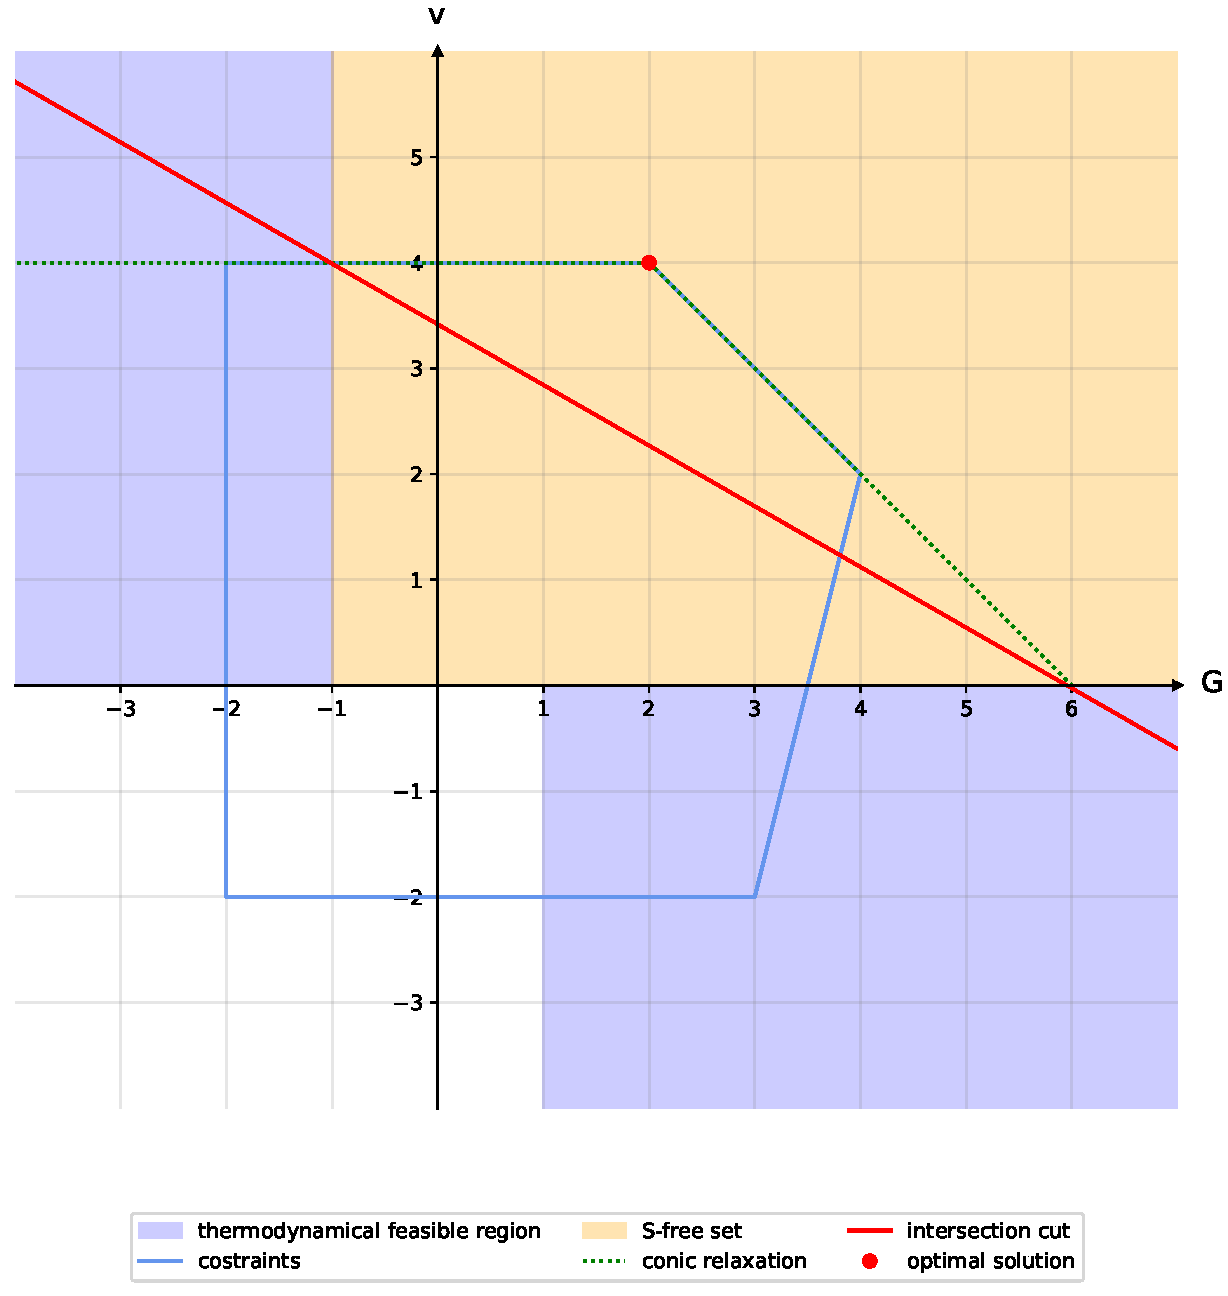
\includegraphics[width=0.8\textwidth]{Images/intersection_cut_ll_fba.pdf}
    \label{fig:intersection_cut_ll_fba}
    \subcaption*{We consider this simple model with constraints in 2D, with $\epsilon=1$. We have the decision variables $v_i, \Delta \mu_i \in \mathbb{R}$, polyhedral constraints $P$ (blue), and the set $S$ (purple area). The intersection of $S$ and $P$ is the true feasible region. Let $(\tilde{\Delta \mu}_i, \tilde v_i)$ of the optimal solution to the relaxed problem be at $(2,4)$. As $\tilde{\Delta \mu}_i$ and $\tilde v_i$ are both positive, $C_1$ is a maximal $S$-free set (yellow area). The conic relaxation at $(\tilde{\Delta \mu}_i, \tilde v_i)$ and the S-free set $C_1$ intersect at the points $(-1,4)$ and $(6,0)$. The area between the line through the intersecting points and $(\tilde{\Delta \mu}_i, \tilde v_i)$ is cut off.}
\end{figure}
% thermo_fba_bigM
\todo[inline]{make figure nice, correct labels, colour interior of polytope, fix cut off extreme ray, correct subsection}

The conic relaxation $P'$ at a relaxed solution $\boldsymbol{\tilde x}$ is a cone with apex $\boldsymbol{\tilde x}$ the extreme rays are the intersections of the active constraints. $P'$ can be written as a conic combination of extreme rays \cref{Eq:conic_relaxation} or as a polyhedron of the active constraints \cref{Eq:conic_relaxation_polyhedral}. The basic variables and nonbasic constraints defining a basis $P'$ for $\boldsymbol{\tilde x}$ can be extracted from an LP solver. 

Suppose reaction $i$ in $\boldsymbol{\tilde x}$ has $\tilde v_i >0$ and $\tilde{\Delta \mu_i} >- \epsilon$. $(\tilde v_i, \tilde{\Delta \mu_i}) \in C_1$ and $(\tilde v_i, \tilde{\Delta \mu_i}) \not \in C_2$. % and therefore $C_1$ is a maximal $S$-free set around $\tilde x$.
To compute the intersection of the conic relaxation and $C_1$, we check for each extreme ray $\bold r^j = (- \bold{\tilde A}^{-1}_{*,j})$ generated by $\tilde x$ whether it intersects the boundary of $C_1$. 
First, the intersection of the conic relaxation with the hyperplane $h_1 = \{\bold x \in \mathbb{R}^{n + m + |\mathcal{I}|} \, | \, v_i = 0 \} $ is computed. $(\boldsymbol{\tilde x} + \lambda_1 \bold r^j)_{k_1} = \bold 0$ is solved for $\lambda_1$, where $k_1$ corresponds to the index of $v_i$ in $\boldsymbol{\tilde x}$.
% Each ray $r^j$ generated by $\tilde x$ is set equal to $h_1$ and solved for $\lambda_1$: $\tilde x + \lambda_1 r^j=h_1$. 

Similarly, the intersection of each extreme ray generated by $\boldsymbol{\tilde x}$ with $h_2$ is computed, where $h_2 = \{\bold x \in \mathbb{R}^{n + m + |\mathcal{I}|} \, | \, \Delta \mu_i = -\epsilon \}$. We solve $(\boldsymbol{\tilde x} + \lambda_2 \bold r^j)_{k_2} = -\boldsymbol \epsilon$ for the step size $\lambda_2$, where $k_2$ is the index of $\Delta \mu_i$ in $\boldsymbol{\tilde x}$. 
An extreme ray intersects the boundary of $C_1$ if either $\lambda_1$ or $\lambda_2$ is finite and positive. If $\lambda_1, \lambda_2$ are both negative or if the ray does not intersect with either of the lines, there is no intersection with $C_1$ and the step size is set to $\infty$. 
\todo[inline]{explain what happens if lambda is zero or very small, or if lines are almost parallel \\ explain the geometric meaning of infinity case}

If reaction $i$ in $\tilde x$ has $v_i <0$ and $\Delta \mu_i < \epsilon$, the intersection between the conic relaxation and $C_2$ is computed analogously. The equations to solve are $(\boldsymbol{\tilde x} + \lambda_1 \bold r^j)_{k_1} = \bold 0$ and $(\boldsymbol{\tilde x} + \lambda_1 \bold r^j)_{k_2} = \boldsymbol \epsilon$.

% Suppose we have one reaction and $v, \Delta \mu \in \mathbb{R}$ which have positive values assigned. The $S$-free set $C_1$ contains the points that are greater than $s_1 = \begin{pmatrix} 1 \\ 0 \end{pmatrix} t_1$ and greater than $s_2 = \begin{pmatrix} -1 \\ 0
% \end{pmatrix} + \begin{pmatrix} 0 \\ 1 \end{pmatrix} t_2$ \todo[inline]{make vector nice}. First, the intersection of the conic relaxation with the line $s_1$ is computed. Each ray $r^j$ generated by $\tilde x$ is set equal to $s_1$ and solved for $\lambda_1$: $\tilde + \lambda_1 r^j=s_1$. Analogously, each ray generated by $\tilde x$ is set equal to $s_2$ and the step size is denoted as $\lambda_2$. The intersection with the boundary of $C_1$ is the minimum of positive $\lambda_1$ and $\lambda_2$. If $\lambda_1, \lambda_2$ are both negative or if the ray does not intersect with either of the lines, there is no intersection with $C_1$ and the step size is set to $- \infty$.
% In higher dimensions, the $S$-free set  of reaction $i$ with $v_i > 0$ and $\Delta \mu_i > -1$ is still the intersection of the two half-spaces $C_1 = \{(v, \Delta \mu) | v_i \geq 0, \, \Delta \mu_i \geq -1\}$.

% There are at least two possibilities of using intersection cuts: (1) one can either decompose the problem to solve FBA ... \todo[inline]{depends on definition of $P$} and generate cuts based on a solution to the master problem or 
% (2) one could also compute several intersection cuts from an FBA solution and add the cuts to the ll-FBA problem. 

\todo[inline]{write about possible usage of intersection cut}
\todo[inline]{write about conic relaxation extraction in detail}
\todo[inline]{example}

\subsection{Disjunctive Programming} \label{section:disjunctive_programming}
\cref{problem:llfba} written as disjunctive program is:

\begin{maxi!}
    {\scriptstyle \bold v, \boldsymbol{\Delta \mu}, \boldsymbol \mu}{\bold c^\intercal \bold v}{\label[problem]{problem:llfba_dp}}{}
    \addConstraint{\bold S \bold v= \bold 0} 
    \addConstraint{\bold l \leq \bold v \leq \bold u}
    \addConstraint{\boldsymbol{\Delta \mu}^\intercal = \boldsymbol \mu^\intercal \bold S_{\mathcal{I}}}
    \addConstraint{
        \left[\begin{array}{cc} Y_i \\ v_i \geq 0 \\ \Delta \mu_i \leq -\epsilon \end{array} \right] \lor 
        \left[\begin{array}{cc} Y_{i + |\mathcal{I}|} \\ v_i \leq 0 \\ \Delta \mu_i \geq \epsilon \end{array} \right] 
        \quad \forall i \in \mathcal{I}} \label[constraint]{constraint:llfba_dp_e}
    \addConstraint{Y_i \lor Y_{i + |\mathcal{I}|} \quad \forall i \in \mathcal{I}} \label[constraint]{constraint:llfba_dp_f}
\end{maxi!}
\quad where we have Boolean variables $Y_i \in \{true, false \}$ in addition to the continuous variables $\bold v \in \mathbb{R}^n, \boldsymbol{\Delta \mu} \in \mathbb{R}^{| (\mathcal{I})|}, \boldsymbol \mu \in \mathbb{R}^m$. %\todo[inline]{explain why you name it Boolean and not binary}

The \textsf{DisjunctiveProgramming} package extends \textsf{JuMP} and enables formulating disjunctive programs and provides several MIP reformulations \cite{perez_disjunctiveprogrammingjl_2023}
. The package is used to model \cref{problem:llfba_dp} and to acquire the big-M reformulation and the hull reformulation (see \cref{section:solving_dps}). For both reformulations the Boolean variable $Y_i$ is modeled by a binary variable $y_i$. \cref{constraint:llfba_dp_f} is then:
\begin{equation*}
    y_i + y_{i + |\mathcal{I}|} = 1 \quad \forall i \in \mathcal{I}
\end{equation*}

The big-M reformulation of \cref{constraint:llfba_dp_e} is:
\begin{align*}
    -v_i &\leq M (1 - y_i) \\
    v_i &\leq M (1- y_{i + |\mathcal{I}|}) \\
    \Delta \mu_i &\leq -\epsilon + M (1 - y_i) \\ 
    - \Delta \mu_i &\leq -\epsilon + M(1 - y_{i + |\mathcal{I}|})
\end{align*}

\quad which is identical to \cref{problem:thermo_fba_bigM} except that the big-M reformulation of \cref{problem:llfba_dp} uses two binary variables per disjunction instead of one.
The tightness of the relaxed feasible solution of the big-M reformulation depends on the scalar $M$. The package finds the optimal value of $M$ by using interval arithmetic \cite{hutchison_automating_2010}.

For the hull reformulation, two continuous variables are added for each decision variable in a disjunction. The variables corresponding to $v_i$ are denoted as $v_{i_1}$ and $v_{i_2}$ and the variables corresponding to $\Delta \mu_i$ are $\Delta \mu_{i_1}$ and $\Delta \mu_{i_2}$. The hull reformulation of \cref{constraint:llfba_dp_e} is:
\begin{align*}
    &v_i = v_{i_1} + v_{i_2} \\
    &\Delta \mu_i = \Delta \mu_{i_1} + \Delta \mu_{i_2} \\
    &v_{i_1} \leq 0 \\
    &v_{i_2} \leq 0 \\
    &\Delta \mu_{i_1} \leq - y_i \\ 
    &- \Delta \mu_{i_2} \leq -y_{i + |\mathcal{I}|} \\
    &y_i + y_{i + |\mathcal{I}|} = 1 \\
    &0 \leq v_{i_j} \leq M v_{i_j}  \quad \forall j \in \{1,2\}
\end{align*}

We see that the hull reformulation needs more decision variables and constraints than the big-M reformulation. However, the feasible region of the hull reformulation is the convex hull of the disjunctions and therefore the tightest possible convex approximation. 

% \subsection{Solvers and Packages} \label{section:solvers_packages}
% All experiments were carried out on an 8-core compute node equipped with an Intel Xeon E3-1245v5 3.50GHz CPU and 32GB RAM. We use Julia 1.7.0. The package versions used are FrankWolfe.jl v.0.2.15, Bonobo.jl v0.1.2, SCIP.jl v0.11.8

\subsection{Models} \label{section:models}
\subsubsection{BiGG}
We use a subset of metabolic networks of the \textit{biochemical, genetic, and genomic} (BiGG) database \cite{BiGG}. The models selected cover the different model sizes the smallest being \textsf{e\_coli\_core} and the largest \textsf{Recon3D}. \cref{Tab:big_model_size} lists the models including the number of metabolites and the number of reactions.

\subsubsection{Yeast}

\subsubsection{GECKO}
When adding enzyme constraints to the model, the flux rate depends on the enzymes and the flux bounds $\bold l, \bold u$ are only required to restrict the direction of a reaction.  
We use COBREXA to build the enzyme models, and we generate the enzyme data randomly.
The turnover numbers differentiate for the forward and backward direction of a reaction and therefore we split each reversible reactions into one forward and one backward reaction.
At least one enzyme is mapped to each reaction including the turnover numbers for the reaction in the forward and the turnover number for the backward direction are defined. 
%We only consider reactions involving genes, because \unsure[inline]{why?}. 
The turnover numbers are taken from a normal distribution. %10^rand(Normal(μ,1))
The protein concentrations have to be in the interval $[0, 1000]$ %\todo[inline]{gene product = protein}
. An enzyme is made up of one or more proteins.
Each protein is randomly associated with either mass group A or B, and the product mass of each group is bounded by 0.5 mml/gDW. For each protein we assign a product molar mass randomly from a Uniform distribution. 
The stoichiometric matrix including enzyme data $\bold S^{GECKO}$ has a row for each metabolite and for each protein in the nework. The columns are the metabolic reactions in addition to an enzyme balance constraint linking each isozyme to its protein compound and the reaction it catalyzes.
\todo[inline]{enzymes are protein compounds}

% gene product mass group: maps gene products to specific capacity bound IDs (each genes(model) randomly assigned to group A o B),
% gene product molar mass: molar mass of a gene product (rand(Uniform(10, 100)) for each genes(model)),
% gene product mass group bound: numeric bound of each capacity ID  (0.5 mml/gDW each)
% \unsure[inline]{genes in metabolic network?}
The size of $\bold S^{GECKO}$ is therefore much larger than $\bold S$.
As an example, the stoichiometric matrix of \textsf{e\_coli\_core} including enzyme data is of size $\mathbb{R}^{209 \times 334}$. The number of rows results from 72 metabolites and 137 proteins, and we have 334 columns, instead of 95. 
\begin{table}[!ht]
    \centering
    \begin{tabular}{lll}
    \hline
        \textbf{organism} & \textbf{\# metabolites} & \textbf{\# reactions} \\ \hline
        e\_coli\_core & 72 & 95 \\ 
        iAB\_RBC\_283 & 342 & 469 \\ 
        iIS312\_Amastigote & 606 & 519 \\ 
        iAF692 & 628 & 690 \\ 
        iSB619 & 655 & 743 \\ 
        iNF517 & 650 & 754 \\ 
        iHN637 & 698 & 785 \\ 
        iJB785 & 768 & 849 \\ 
        iNJ661 & 825 & 1025 \\ 
        iSynCJ816 & 928 & 1044 \\ 
        iJN746 & 907 & 1054 \\ 
        iJR904 & 761 & 1075 \\ 
        iEK1008 & 998 & 1226 \\ 
        iCN900 & 885 & 1229 \\ 
        iYO844 & 990 & 1250 \\ 
        iND750 & 1059 & 1266 \\ 
        iMM904 & 1226 & 1577 \\ 
        iRC1080 & 1706 & 2191 \\ 
        iAF1260 & 1668 & 2382 \\ 
        iSDY\_1059 & 1888 & 2539 \\ 
        STM\_v1\_0 & 1802 & 2545 \\ 
        iJO1366 & 1805 & 2583 \\ 
        iSbBS512\_1146 & 1910 & 2591 \\ 
        iS\_1188 & 1914 & 2619 \\ 
        iSFV\_1184 & 1917 & 2621 \\ 
        iSF\_1195 & 1917 & 2630 \\ 
        iSFxv\_1172 & 1918 & 2638 \\ 
        iML1515 & 1877 & 2712 \\ 
        iZ\_1308 & 1923 & 2721 \\ 
        iAPECO1\_1312 & 1942 & 2735 \\ 
        iECB\_1328 & 1951 & 2748 \\ 
        iETEC\_1333 & 1962 & 2756 \\ 
        iYS1720 & 2436 & 3357 \\ 
        iMM1415 & 2775 & 3726 \\ 
        RECON1 & 2766 & 3741 \\ 
        iLB1027\_lipid & 2172 & 4456 \\ 
        Recon3D & 5835 & 10600 \\ \hline
    \end{tabular}
    \caption{\label{Tab:big_model_size} Model size of used BiGG models.}
\end{table}
\unsure[inline]{organisms in textsf?}
\clearpage
\section{Discussion}
\todo[inline]{how to handle suboptimally solved instances}

\subsection{FBA and ll-FBA Variants}
\begin{figure}[h!]
    \caption{performance of ll-FBA variants}
    \centering
    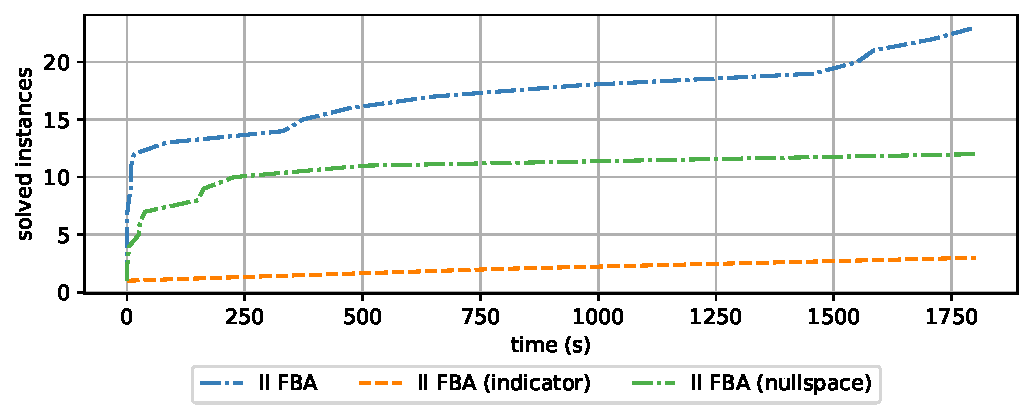
\includegraphics[width=1.0\textwidth]{Images/fba_variants_comparison_plot.pdf}
    \label{fig:ll_fba_comparion}
    \subcaption*{The results are shown in \cref{tab:ll_fba_comparison} and in \cref{tab:ll_fba_indicator}}
\end{figure}

% \begin{table}[!ht]
%     \centering
%     \begin{tabular}{|l|l|l|l|l|l|l|l|}
%     \hline
%         \thead{organism} & \thead{type} & \thead{objective} & \thead{dual bound} & \thead{termination} & \thead{time limit} & \thead{time (s)} & \thead{nodes} \\ \hline
%         iAF692 & loopless\_fba & 0.0268 & 0.0268 & OPTIMAL & 1800 & 4.51 & 351 \\ \hline
%         iAF692 & loopless\_fba\_nullspace & 0.0256 & 0.0268 & TIME\_LIMIT & 1800 & 1800.0 & 575 \\ \hline
%         iAF692 & loopless\_indicator\_fba & 0.0268 & 0.0268 & OPTIMAL & 1800 & 1285.4 & 11532 \\ \hline
%         iJR904 & loopless\_fba & 0.9219 & 0.9219 & OPTIMAL & 1800 & 114.67 & 7614 \\ \hline
%         iJR904 & loopless\_fba\_nullspace & 0.9219 & 0.9219 & OPTIMAL & 1800 & 172.86 & 641 \\ \hline
%         iJR904 & loopless\_indicator\_fba & 0.0 & 0.9219 & TIME\_LIMIT & 1800 & 1800.0 & 31243 \\ \hline
%         iML1515 & loopless\_fba & 0.865 & 0.877 & TIME\_LIMIT & 1800 & 1800.0 & 12098 \\ \hline
%         iML1515 & loopless\_fba\_nullspace & NaN & NaN & TIME\_LIMIT & 1800 & 1800.06 & 15 \\ \hline
%         iML1515 & loopless\_indicator\_fba & NaN & NaN & TIME\_LIMIT & 1800 & 1800.38 & 6776 \\ \hline
%     \end{tabular}
% \end{table}

\subsection{Blocking Cycles in FBA}
\begin{figure}[h!]
    \caption{runtime of ll-FBA and ll-FBA with blocked cycles}
    \centering
    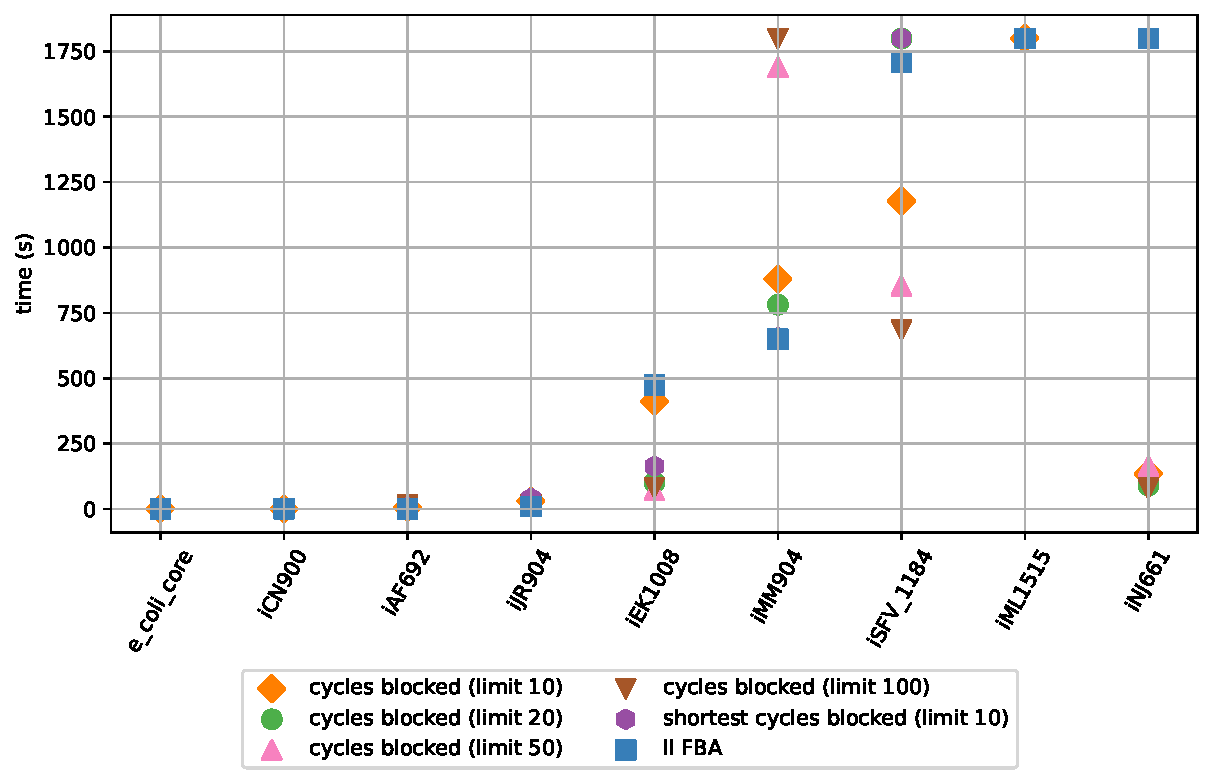
\includegraphics[width=1.0\textwidth]{Images/cff_comparison.pdf}
    \label{fig:cff_comparison}
    \subcaption*{The results are shown in \cref{tab:cff} and \cref{tab:cff_shortest_cycles}}
\end{figure}

% \begin{table}[!ht]
%     \centering
%     \begin{tabular}{|l|l|l|l|l|l|}
%     \hline
%     \thead{\textbf{iAF692}} & \thead{objective} & \thead{status} & \thead{blocked cycles} & \thead{time (s)} & \thead{nodes} \\ \hline
%         loopless\_fba\_blocked & 0.0268 & OPTIMAL & 50 & 7.33 & 1699 \\ \hline
%         loopless\_fba\_blocked & 0.0268 & OPTIMAL & 100 & 6.51 & 818 \\ \hline
%         loopless\_fba\_blocked\_shortest\_cycles & 0.0268 & OPTIMAL & 50 & 7.34 & 1528 \\ \hline
%         loopless\_fba\_blocked\_shortest\_cycles & 0.0268 & OPTIMAL & 100 & 6.39 & 917 \\ \hline
%     \end{tabular}
% \end{table}

% \begin{table}[!ht]
%     \centering
%     \begin{tabular}{|l|l|l|l|l|l|}
%     \hline
%     \thead{\textbf{iJR904}} & \thead{objective} & \thead{status} & \thead{blocked cycles} & \thead{time (s)} & \thead{nodes} \\ \hline
%         loopless\_fba\_blocked & 0.9219 & OPTIMAL & 50 & 92.41 & 6505 \\ \hline
%         loopless\_fba\_blocked & 0.9219 & OPTIMAL & 100 & 48.27 & 2314 \\ \hline
%         loopless\_fba\_blocked\_shortest\_cycles & 0.9219 & OPTIMAL & 50 & 73.95 & 5777 \\ \hline
%         loopless\_fba\_blocked\_shortest\_cycles & 0.9219 & OPTIMAL & 100 & 30.22 & 365 \\ \hline
%     \end{tabular}
% \end{table}

% \begin{sidewaystable}
%     \begin{tabular}{|l|l|l|l|l|l|l|l|l|}
%     \hline
%         \thead{\textbf{iAF692}} & \thead{objective} & \thead{dual} & \thead{status} & \thead{blocked cycles} & \thead{ceiling} & \thead{block limit} & \thead{time (s)} & \thead{nodes} \\ \hline
%         loopless\_fba & 0.0268 & 0.0268 & OPTIMAL & ~ & ~ & ~ & 4.51 & 351 \\ \hline
%         loopless\_fba\_nullspace & 0.0256 & 0.0268 & TIME\_LIMIT & ~ & ~ & ~ & 1800.0 & 575 \\ \hline
%         loopless\_indicator\_fba & 0.0268 & 0.0268 & OPTIMAL & ~ & ~ & ~ & 1285.4 & 11532 \\ \hline
%         loopless\_indicator\_fba\_blocked\_same\_objective & 0.0268 & 0.0268 & OPTIMAL & 0 & 50 & 500 & 1286.58 & 11532 \\ \hline
%         loopless\_indicator\_fba\_blocked\_same\_objective & 0.0268 & 0.0268 & OPTIMAL & 0 & 100 & 500 & 1269.63 & 11532 \\ \hline
%         loopless\_fba\_blocked\_same\_objective & 0.0268 & 0.0268 & OPTIMAL & 0 & 50 & 100 & 4.53 & 351 \\ \hline
%         loopless\_fba\_blocked\_same\_objective & 0.0268 & 0.0268 & OPTIMAL & 0 & 100 & 100 & 4.51 & 351 \\ \hline
%         loopless\_fba\_blocked\_same\_objective & 0.0268 & 0.0268 & OPTIMAL & 0 & 200 & 100 & 4.51 & 351 \\ \hline
%         loopless\_fba\_blocked\_same\_objective & 0.0268 & 0.0268 & OPTIMAL & 0 & 500 & 100 & 4.5 & 351 \\ \hline
%         loopless\_fba\_blocked & 0.0268 & 0.0268 & OPTIMAL & 7 & 50 & 100 & 6.08 & 949 \\ \hline
%         loopless\_fba\_blocked & 0.0268 & 0.0268 & OPTIMAL & 7 & 100 & 100 & 6.09 & 949 \\ \hline
%         loopless\_fba\_blocked & 0.0268 & 0.0268 & OPTIMAL & 7 & 200 & 100 & 6.1 & 949 \\ \hline
%         loopless\_fba\_blocked & 0.0268 & 0.0268 & OPTIMAL & 7 & 500 & 100 & 6.07 & 949 \\ \hline
%         loopless\_fba\_blocked00 & 0.0268 & 0.0268 & OPTIMAL & 50 & 10000 & 50 & 7.34 & 1699 \\ \hline
%         loopless\_fba\_blocked00 & 0.0268 & 0.0268 & OPTIMAL & 100 & 10000 & 100 & 6.49 & 818 \\ \hline
%         loopless\_fba\_blocked\_shortest\_cycles00 & 0.0268 & 0.0268 & OPTIMAL & 50 & 10000 & 50 & 7.76 & 1528 \\ \hline
%         loopless\_fba\_blocked\_shortest\_cycles00 & 0.0268 & 0.0268 & OPTIMAL & 100 & 10000 & 100 & 6.38 & 917 \\ \hline
%     \end{tabular}


%     \vspace{5mm}

%     \begin{tabular}{|l|l|l|l|l|l|l|l|l|l|}
%     \hline
%         \thead{\textbf{iJR904}} & \thead{objective} & \thead{dual} & \thead{status} & \thead{blocked cycles} & \thead{ceiling} & \thead{block limit} & \thead{time (s)} & \thead{nodes} \\ \hline
%         loopless\_fba & 0.9219 & 0.9219 & OPTIMAL & ~ & ~ & ~ & 114.67 & 7614 \\ \hline
%         loopless\_fba\_nullspace & 0.9219 & 0.9219 & OPTIMAL & ~ & ~ & ~ & 172.86 & 641 \\ \hline
%         loopless\_indicator\_fba & 0.0 & 0.9219 & TIME\_LIMIT & ~ & ~ & ~ & 1800.0 & 31243 \\ \hline
%         loopless\_indicator\_fba\_blocked\_same\_objective & 0.0 & 0.9219 & TIME\_LIMIT & 0 & 50 & 500 & 1800.0 & 28423 \\ \hline
%         loopless\_indicator\_fba\_blocked\_same\_objective & 0.0 & 0.9219 & TIME\_LIMIT & 0 & 100 & 500 & 1800.0 & 28283 \\ \hline
%         loopless\_fba\_blocked\_same\_objective & 0.9219 & 0.9219 & OPTIMAL & 0 & 50 & 100 & 115.01 & 7614 \\ \hline
%         loopless\_fba\_blocked\_same\_objective & 0.9219 & 0.9219 & OPTIMAL & 0 & 100 & 100 & 114.7 & 7614 \\ \hline
%         loopless\_fba\_blocked\_same\_objective & 0.9219 & 0.9219 & OPTIMAL & 0 & 200 & 100 & 114.14 & 7614 \\ \hline
%         loopless\_fba\_blocked\_same\_objective & 0.9219 & 0.9219 & OPTIMAL & 0 & 500 & 100 & 110.62 & 7614 \\ \hline
%         loopless\_fba\_blocked & 0.9219 & 0.9219 & OPTIMAL & 13 & 50 & 100 & 89.4 & 4804 \\ \hline
%         loopless\_fba\_blocked & 0.9219 & 0.9219 & OPTIMAL & 20 & 100 & 100 & 45.61 & 881 \\ \hline
%         loopless\_fba\_blocked & 0.9219 & 0.9219 & OPTIMAL & 60 & 200 & 100 & 101.19 & 28 \\ \hline
%         loopless\_fba\_blocked & 0.9219 & 0.9219 & OPTIMAL & 100 & 500 & 100 & 48.43 & 2314 \\ \hline
%         loopless\_fba\_blocked00 & 0.9219 & 0.9219 & OPTIMAL & 50 & 10000 & 50 & 99.55 & 6505 \\ \hline
%         loopless\_fba\_blocked00 & 0.9219 & 0.9219 & OPTIMAL & 100 & 10000 & 100 & 48.28 & 2314 \\ \hline
%         loopless\_fba\_blocked\_shortest\_cycles00 & 0.9219 & 0.9219 & OPTIMAL & 50 & 10000 & 50 & 74.12 & 5777 \\ \hline
%         loopless\_fba\_blocked\_shortest\_cycles & 0.9219 & 0.9219 & OPTIMAL & 13 & 50 & 100 & 87.25 & 2792 \\ \hline
%     \end{tabular}
% \end{sidewaystable}

% \begin{sidewaystable}
%     \centering
%     \begin{tabular}{|l|l|l|l|l|l|l|l|l|}
%     \hline
%         \thead{\textbf{iML1515}} & \thead{objective} & \thead{dual} & \thead{status} & \thead{blocked cycles} & \thead{ceiling} & \thead{block limit} & \thead{time (s)} & \thead{nodes} \\ \hline
%        loopless\_fba & 0.865 & 0.877 & TIME\_LIMIT & ~ & ~ & ~ & 1800.0 & 12098 \\ \hline
%         loopless\_fba\_nullspace & NaN & NaN & TIME\_LIMIT & ~ & ~ & ~ & 1800.06 & 15 \\ \hline
%         loopless\_indicator\_fba & NaN & NaN & TIME\_LIMIT & ~ & ~ & ~ & 1800.38 & 6776 \\ \hline
%         loopless\_indicator\_fba\_blocked\_same\_objective & NaN & NaN & TIME\_LIMIT & 50 & 50 & 500 & 1800.0 & 8902 \\ \hline
%         loopless\_indicator\_fba\_blocked\_same\_objective & NaN & NaN & TIME\_LIMIT & 100 & 100 & 500 & 1800.56 & 6828 \\ \hline
%         loopless\_fba\_blocked\_same\_objective & 0.0 & 0.877 & TIME\_LIMIT & 50 & 50 & 100 & 1800.0 & 41468 \\ \hline
%         loopless\_fba\_blocked\_same\_objective & 0.0 & 0.877 & TIME\_LIMIT & 100 & 100 & 100 & 1800.0 & 51433 \\ \hline
%         loopless\_fba\_blocked\_same\_objective & 0.0 & 0.877 & TIME\_LIMIT & 100 & 200 & 100 & 1800.0 & 52372 \\ \hline
%         loopless\_fba\_blocked\_same\_objective & 0.0 & 0.877 & TIME\_LIMIT & 100 & 500 & 100 & 1800.05 & 52039 \\ \hline
%         loopless\_fba\_blocked & 0.0 & 0.877 & TIME\_LIMIT & 50 & 50 & 100 & 1800.0 & 45557 \\ \hline
%         loopless\_fba\_blocked & 0.0 & 0.877 & TIME\_LIMIT & 100 & 100 & 100 & 1800.0 & 41023 \\ \hline
%         loopless\_fba\_blocked & 0.0 & 0.877 & TIME\_LIMIT & 100 & 200 & 100 & 1800.0 & 40683 \\ \hline
%         loopless\_fba\_blocked & 0.0 & 0.877 & TIME\_LIMIT & 100 & 500 & 100 & 1800.0 & 40864 \\ \hline
%         loopless\_fba\_blocked\_shortest\_cycles & 0.2277 & 0.877 & TIME\_LIMIT & 50 & 50 & 100 & 1800.04 & 48769 \\ \hline
%     \end{tabular}
% \end{sidewaystable}

\subsection{No-Good Cuts}
\begin{figure}[h!]
    \caption{runtime of ll-FBA and ll-FBA with no-good cuts}
    \centering
    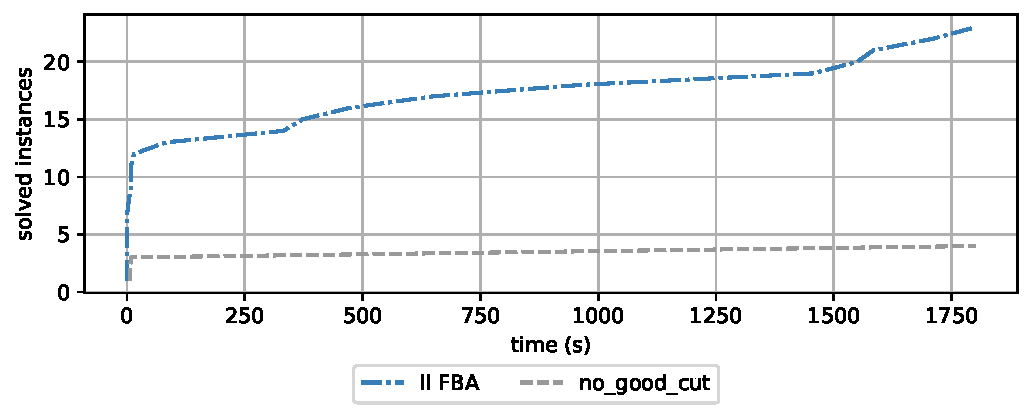
\includegraphics[width=1.0\textwidth]{Images/no_good_cuts_comparison_plot.pdf}
    \label{fig:cff_comparison}
    \subcaption*{The results are shown in \cref{tab:no_good_cuts}}
\end{figure}

\subsection{Combinatorial Benders' Cuts}

\begin{figure}[h!]
    \caption{solved instances by CB (indicator) and ll-FBA}
    \centering
    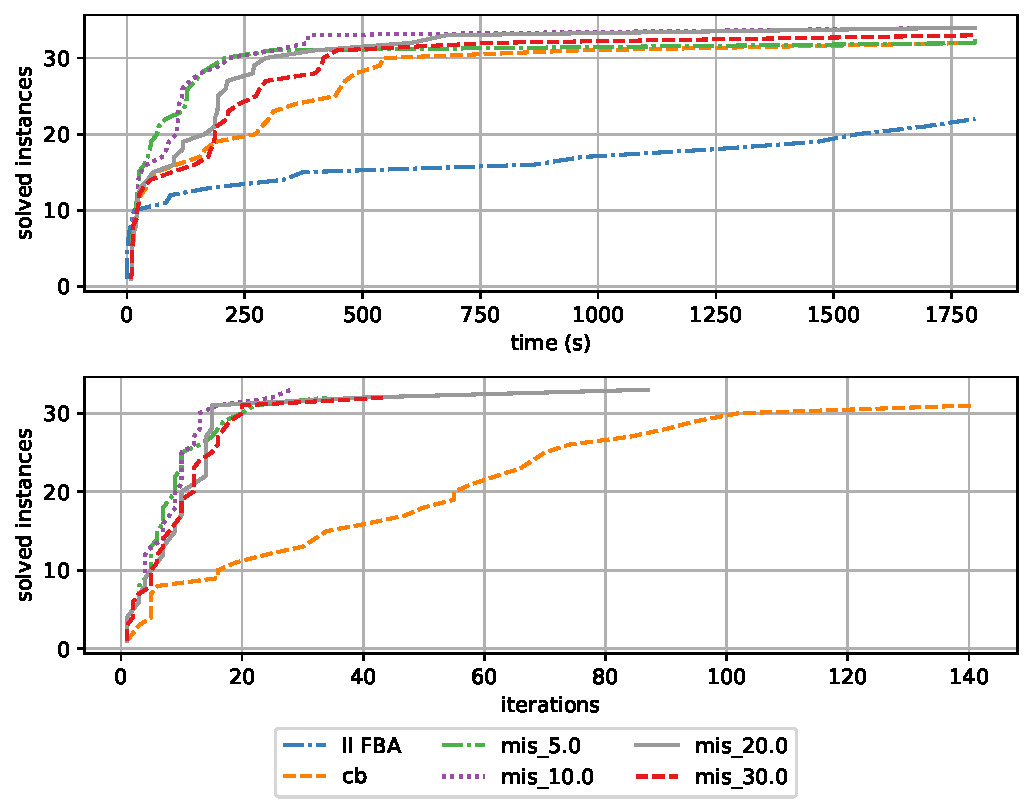
\includegraphics[width=0.8\textwidth]{Images/mis_comparison_solved_instances.pdf}
    \label{fig:mis_comparison_solved_instances}
\end{figure}

\begin{figure}[h!]
    \caption{solved instances by CB (indicator) and ll-FBA}
    \centering
    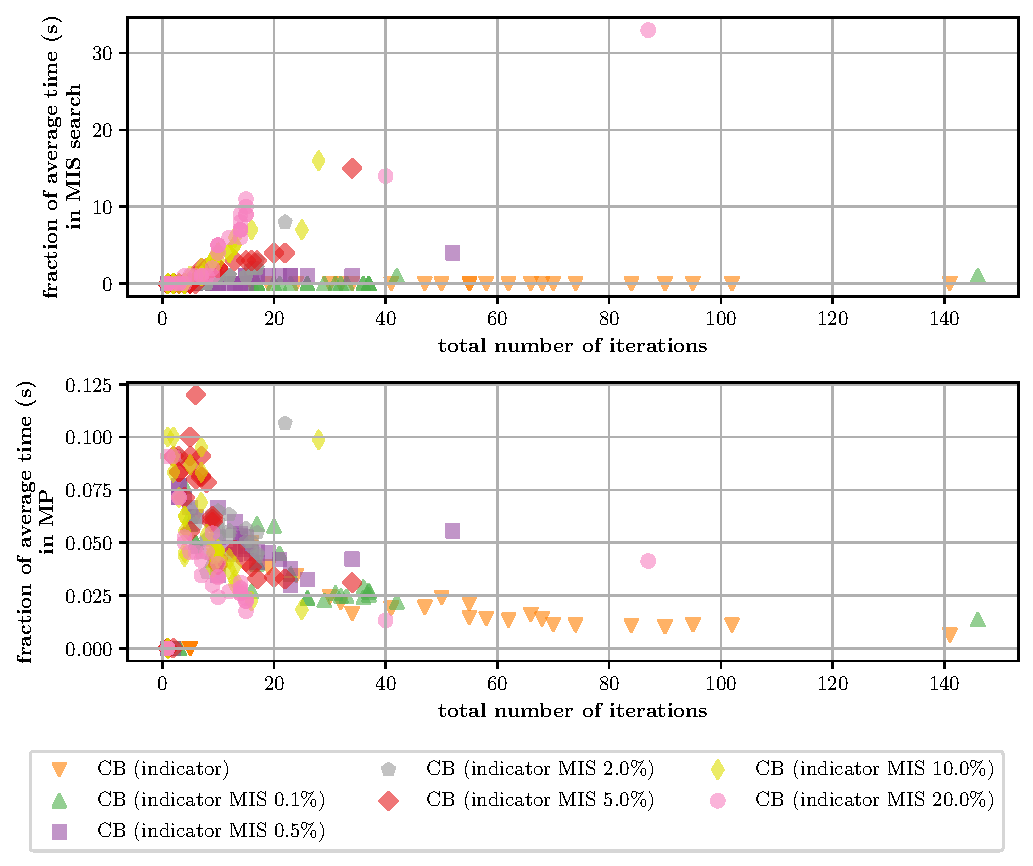
\includegraphics[width=0.8\textwidth]{Images/mis_comparison_time_vs_iterations.pdf}
    \label{fig:mis_comparison_time_vs_iterations}
\end{figure}

\begin{figure}[h!]
    \caption{solved instances by CB (big-M) and ll-FBA}
    \centering
    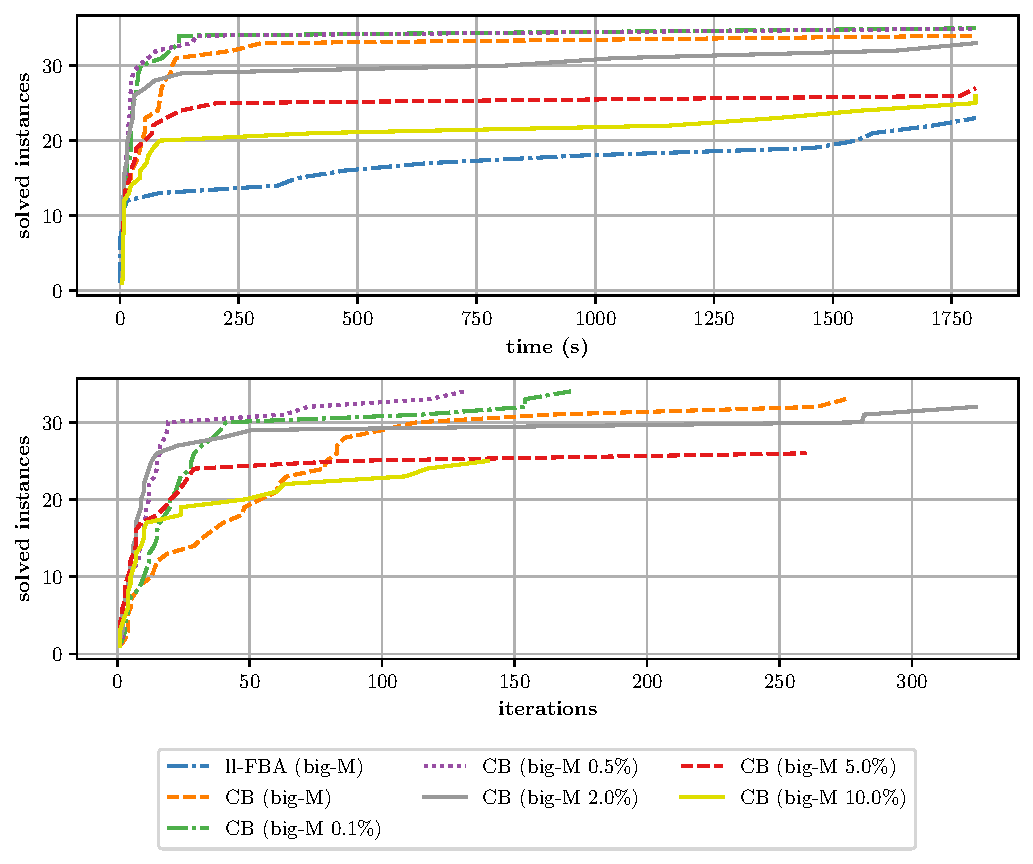
\includegraphics[width=0.8\textwidth]{Images/mis_comparison_solved_instances_big_m.pdf}
    \label{fig:mis_comparison_solved_instances_big_m}
\end{figure}
\todo[inline]{add less cuts}

\begin{figure}[h!]
    \caption{solved instances by CB (big-M) and ll-FBA}
    \centering
    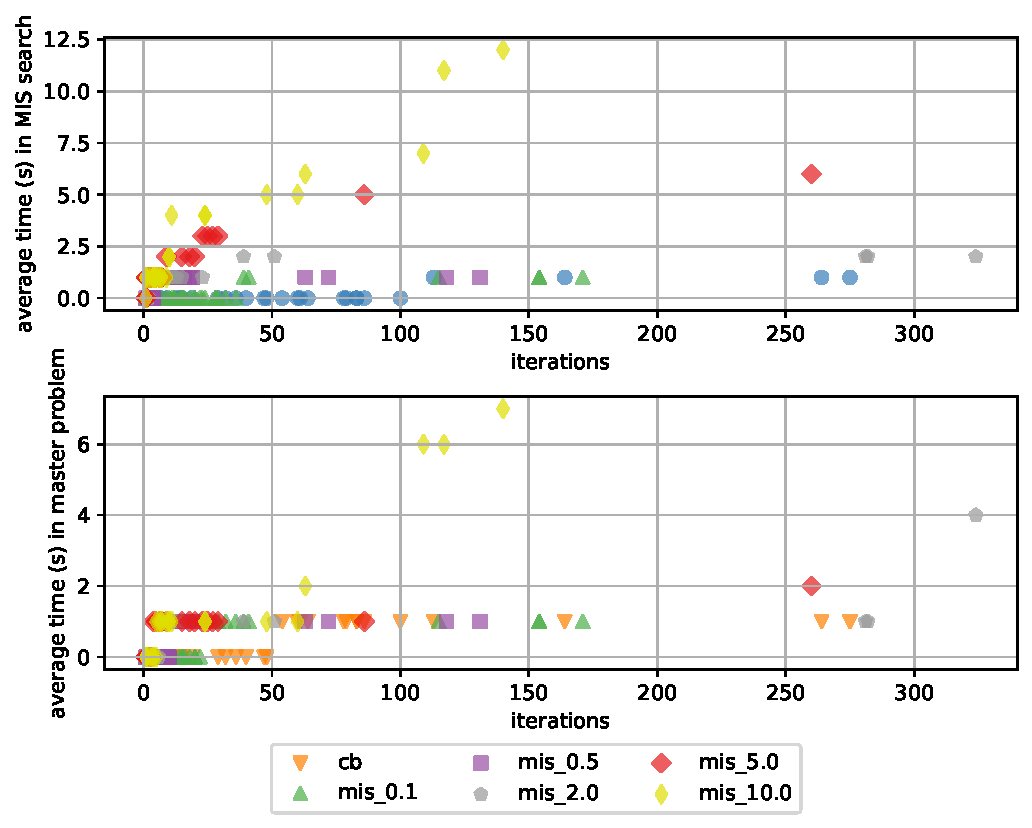
\includegraphics[width=0.8\textwidth]{Images/mis_comparison_time_vs_iterations_big_m.pdf}
    \label{fig:mis_comparison_time_vs_iterations_big_m}
\end{figure}

\begin{figure}[h!]
    \caption{solved instances by CB (big-M), CB (indicator) and CB (indicator and big-M)}
    \centering
    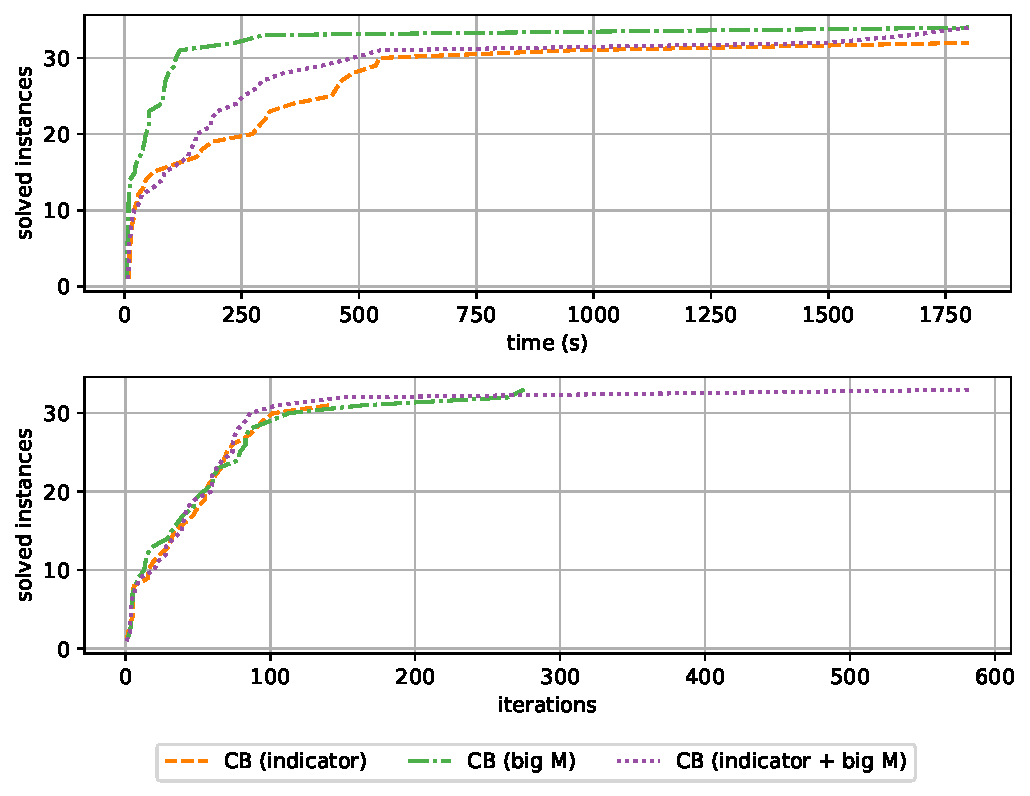
\includegraphics[width=0.8\textwidth]{Images/comparison_solved_instances_indicator_and_big_m.pdf}
    \label{fig:comparison_solved_instances_indicator_and_big_m_as_MP}
\end{figure}

\todo[inline]{note on yeast models}

\begin{figure}[h!]
    \caption{solved GECKO instances by CB (big-M), CB (big-M MIS 5\%) and ll-FBA}
    \centering
    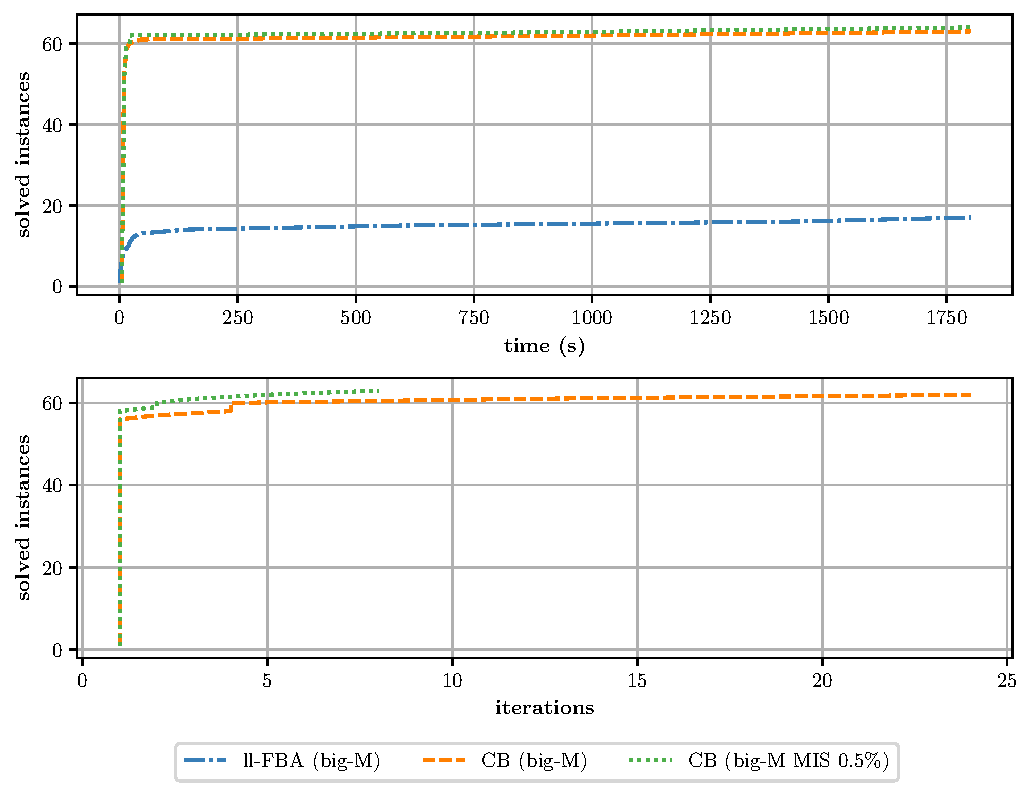
\includegraphics[width=0.8\textwidth]{Images/comparison_solved_instances_gecko_1.0e-8.pdf}
    \label{fig:comparison_gecko}
\end{figure}

\subsection{Intersection Cuts}

\subsection{Disjunctive Programming}

\begin{figure}[h!]
    \caption{solved instances by DP.jl, ll-FBA and CB}
    \centering
    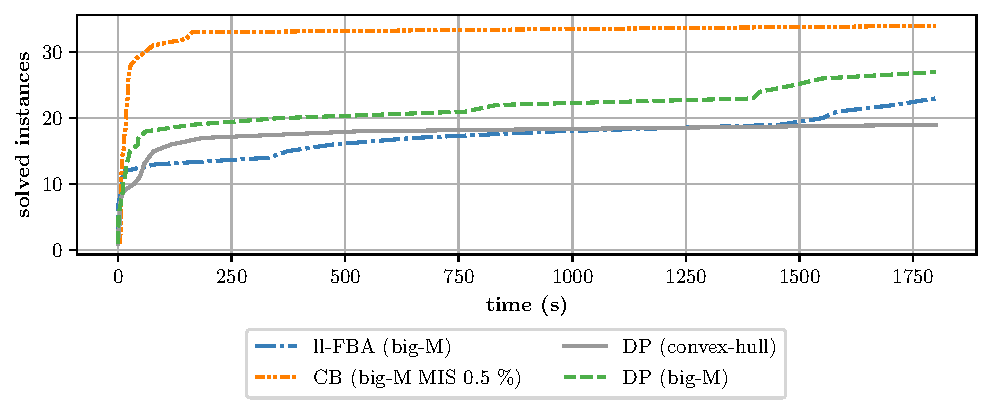
\includegraphics[width=0.8\textwidth]{Images/comparison_dp.pdf}
    \label{fig:}
\end{figure}

\todo[inline]{instances with smaller objective value are considered as NOT SOLVED, update plot}


\clearpage
\section{Conclusion}

% \todo[inline]{future work: improve cut, separation}
% \todo[inline]{constraint handler}
% possible extension to st FBA
% exact LP
% \todo[inline]{move numerically tricky part to LP (MIS search), could use exact LP to MIS search to deal with numerical instability}

\newpage
\todo[inline]{do not enumerate single subsections, only multiple} 
\todo[inline]{use AE or BE consistently} 
\todo[inline]{align all problems that are on the same page} 
\todo[inline]{bold a should look like normal a in bold \\ upright greek symbols ??}
\todo[inline]{page with list of symbols and abbreviations}
\todo[inline]{add var types to mathematical programs}
\todo[inline]{use big-M with vector or scalar}
\todo[inline]{use nonzero}
\todo[inline]{polyhedral $P$, vs primal $\mathbb{P}$ vs optimization problem P, $\mathcal{P}$}
\todo[inline]{program vs problem}
\todo[inline]{fix cover page} 
\todo[inline]{fix bib entries; mosek ok as reference?}
\todo[inline]{use Latex font in plots}
\todo[inline]{running time instead of runtime}
\todo[inline]{minimal infeasible subset vs subsystem}
\todo[inline]{use report instead of article?}
\todo[inline]{relaxed solution instead of optimal solution to relaxed problem}

% \newpage
\pagestyle{plain}
\newpage
\clearpage
\setlength{\footskip}{30pt}
\setlength\bibitemsep{\baselineskip}
\section*{References}
\printbibliography[heading=none]
\addcontentsline{toc}{section}{References}


% \newpage
% \listoftodos[Notes]

% \newpage

\section*{Eigenständigkeitserklärung}
\addcontentsline{toc}{section}{Eigenständigkeitserklärung}




Hiermit versichere ich, dass ich die Masterarbeit selbstständig verfasst und keine anderen als die angegebenen Quellen und Hilfsmittel benutzt habe, alle Ausführungen, die anderen Schriften wörtlich oder sinngemäß entnommen wurden, kenntlich gemacht sind und die Arbeit in gleicher oder ähnlicher Fassung noch nicht Bestandteil einer Studien- oder Prüfungsleistung war.


% 3,5cm Abstand nach oben
\vspace{100mm}
    %\includegraphics[scale=0.2,right]{Bilder/Unterschrift.png}
    %\newline
    
% \begin{figure}[ht]
%     \begin{flushright}% or better \raggedleft see comments below
%     \includegraphics[scale=0.25]{Bilder/Unterschrift.png}
%   %\caption{\texttt{flushright}}
%     \end{flushright}
% \end{figure}

% Ort, Datum
\begin{otherlanguage}{ngerman}
% \noindent{}Berlin, den 17. September 2020
\myformat{\today}
\end{otherlanguage}
% 8 cm breite Linie für die Unterschrift
\begin{minipage}[t]{8cm} 
% gepunktete Linie
\centering \hspace{20mm} \hrulefill \\
% Text unter der Linie
\hspace{20mm} Hannah Troppens
\end{minipage}


\newpage
%Nicht anfassen, so ist der Dokumentenaufbau
% \addtocontents{toc}{\protect\setcounter{tocdepth}{0}}
% \renewcommand{\appendixtocname}{Anhang}
% \addappheadtotoc % Überschrift 'Anhang' in TOC
\renewcommand{\appendixpagename}{Appendix}
\appendix
\appendixpage
\appendixtitleoff
% \section*{Appendix}
% \appendix
\addcontentsline{toc}{section}{Appendix}
\setlength{\footskip}{35pt}

\renewcommand{\figurename}{Appendix Figure}
\renewcommand{\tablename}{Appendix Table}
\setcounter{figure}{0} 
\setcounter{table}{0}
% \crefalias{figure}{appfig}
% \crefalias{table}{apptab}
% \crefalias{section}{appsec}

% ll FBA variants
\begin{table}[!ht]
    \small
    \centering
    \begin{tabular}{@{\extracolsep{4pt}}lllllll@{}}
    \hline
        \multicolumn{1}{c}{} & \multicolumn{3}{c}{\textbf{ll-FBA}} & \multicolumn{3}{c}{\textbf{ll-FBA (nullspace)}}\\ \cline{2-4} \cline{5-7} 
        \textbf{organism} & \textbf{termination} & \textbf{time} & \thead{objective \\value} & \textbf{termination} & \textbf{time} & \thead{objective \\value} \\ \hline
        e\_coli\_core & OPTIMAL & 0 & 0.874 & OPTIMAL & 0 & 0.874 \\
        iAB\_RBC\_283 & OPTIMAL & 0 & 2.936 & OPTIMAL & 2 & 2.936 \\
        iIS312\_Amastigote & OPTIMAL & 0 & 25.339 & OPTIMAL & 0 & 25.339 \\
        iAF692 & OPTIMAL & 0 & 0.0 & TIME\_LIMIT & 1800 & 0.026 \\
        iSB619 & OPTIMAL & 0 & 0.0 & TIME\_LIMIT & 1800 & 0.027 \\
        iNF517 & OPTIMAL & 9 & 0.043 & OPTIMAL & 39 & 0.043 \\
        iHN637 & OPTIMAL & 4 & 0.224 & OPTIMAL & 5 & 0.224 \\
        iJB785 & OPTIMAL & 15 & 0.054 & OPTIMAL & 25 & 0.0 \\
        iNJ661 & TIME\_LIMIT & 1800 & 0.014 & OPTIMAL & 227 & 0.053 \\ 
        iSynCJ816 & OPTIMAL & 1 & 0.0 & INFEASIBLE & 34 & - \\
        iJN746 & OPTIMAL & 332 & 1.4 & TIME\_LIMIT & 1800 & - \\
        iJR904 & OPTIMAL & 9 & 0.0 & OPTIMAL & 163 & 0.922 \\
        iEK1008 & OPTIMAL & 473 & 0.0 & OPTIMAL & 503 & 0.058 \\
        iCN900 & OPTIMAL & 0 & 0.0 & OPTIMAL & 27 & 0.0 \\
        iYO844 & TIME\_LIMIT & 1800 & 0.115 & TIME\_LIMIT & 1800 & 0.0 \\
        iND750 & OPTIMAL & 8 & 0.0 & OPTIMAL & 151 & 0.0 \\
        iMM904 & OPTIMAL & 650 & 0.277 & TIME\_LIMIT & 1800 & 0.0 \\
        iRC1080 & OPTIMAL & 373 & 0.0 & TIME\_LIMIT & 1800 & - \\
        iAF1260 & TIME\_LIMIT & 1800 & 0.0 & TIME\_LIMIT & 1800 & 0.0 \\
        iSDY\_1059 & OPTIMAL & 1457 & 0.938 & TIME\_LIMIT & 1800 & 0.0 \\
        STM\_v1\_0 & TIME\_LIMIT & 1800 & 0.0 & TIME\_LIMIT & 1800 & 0.0 \\
        iJO1366 & TIME\_LIMIT & 1800 & 0.0 & TIME\_LIMIT & 1800 & 0.0 \\
        iSbBS512\_1146 & TIME\_LIMIT & 1800 & 0.0 & TIME\_LIMIT & 1800 & 0.0 \\
        iS\_1188 & TIME\_LIMIT & 1800 & 0.832 & TIME\_LIMIT & 1800 & 0.0 \\
        iSFV\_1184 & OPTIMAL & 1710 & 0.894 & TIME\_LIMIT & 1800 & 0.0 \\
        iSF\_1195 & OPTIMAL & 1584 & 0.915 & TIME\_LIMIT & 1800 & -0.0 \\
        iSFxv\_1172 & OPTIMAL & 966 & 0.894 & TIME\_LIMIT & 1800 & 0.0 \\
        iML1515 & TIME\_LIMIT & 1800 & 0.861 & TIME\_LIMIT & 1800 & - \\
        iZ\_1308 & TIME\_LIMIT & 1800 & 0.0 & TIME\_LIMIT & 1800 & 0.0 \\
        iAPECO1\_1312 & TIME\_LIMIT & 1800 & 0.934 & TIME\_LIMIT & 1800 & 0.0 \\
        iECB\_1328 & TIME\_LIMIT & 1800 & 0.0 & TIME\_LIMIT & 1800 & 0.0 \\
        iETEC\_1333 & TIME\_LIMIT & 1800 & 0.0 & TIME\_LIMIT & 1800 & 0.0 \\
        iYS1720 & TIME\_LIMIT & 1800 & 0.0 & TIME\_LIMIT & 1800 & - \\
        iMM1415 & OPTIMAL & 1550 & 0.0 & TIME\_LIMIT & 1800 & - \\
        RECON1 & OPTIMAL & 83 & 0.0 & TIME\_LIMIT & 1800 & - \\
        iLB1027\_lipid & TIME\_LIMIT & 1800 & 0.0 & TIME\_LIMIT & 1800 & - \\
        Recon3D & TIME\_LIMIT & 1800 & - & TIME\_LIMIT & 1800 & - \\ \hline
    \end{tabular}
    \caption{\label[apptab]{tab:ll_fba_comparison} Results of using the nullspace formulation vs the reformulation.}
\end{table}

\begin{table}[!ht]
    \small
    \centering
    \begin{tabular}{@{\extracolsep{4pt}}lllllll@{}}
    \hline
        \multicolumn{1}{c}{} & \multicolumn{3}{c}{\textbf{ll-FBA (big-M)}} & \multicolumn{3}{c}{\textbf{ll-FBA (indicator)}}\\ \cline{2-4} \cline{5-7} 
        \textbf{organism} & \textbf{termination} & \textbf{time} & \thead{objective \\value} & \textbf{termination} & \textbf{time} & \thead{objective \\value} \\ \hline
        e\_coli\_core & OPTIMAL & 0 & 0.874 & OPTIMAL & 1 & -0.0 \\ \hline
        iAB\_RBC\_283 & OPTIMAL & 0 & 2.936 & TIME\_LIMIT & 1800 & 2.936 \\ \hline
        iIS312\_Amastigote & OPTIMAL & 0 & 25.339 & INFEASIBLE & 1 & - \\ \hline
        iAF692 & OPTIMAL & 0 & 0.0 & TIME\_LIMIT & 1800 & - \\ \hline
        iSB619 & OPTIMAL & 0 & 0.0 & INFEASIBLE & 3 & - \\ \hline
        iNF517 & OPTIMAL & 9 & 0.043 & INFEASIBLE & 7 & - \\ \hline
        iHN637 & OPTIMAL & 4 & 0.224 & INFEASIBLE & 1 & - \\ \hline
        iJB785 & OPTIMAL & 15 & 0.054 & OPTIMAL & 764 & 0.054 \\ \hline
        iNJ661 & TIME\_LIMIT & 1800 & 0.014 & INFEASIBLE & 3 & - \\ \hline
        iSynCJ816 & OPTIMAL & 1 & 0.0 & INFEASIBLE & 0 & - \\ \hline
        iJN746 & OPTIMAL & 332 & 1.4 & TIME\_LIMIT & 1800 & - \\ \hline
        iJR904 & OPTIMAL & 9 & 0.0 & TIME\_LIMIT & 1800 & - \\ \hline
        iEK1008 & OPTIMAL & 473 & 0.0 & TIME\_LIMIT & 1800 & - \\ \hline
        iCN900 & OPTIMAL & 0 & 0.0 & INFEASIBLE & 8 & - \\ \hline
        iYO844 & TIME\_LIMIT & 1800 & 0.115 & TIME\_LIMIT & 1800 & - \\ \hline
        iND750 & OPTIMAL & 8 & 0.0 & INFEASIBLE & 61 & - \\ \hline
        iMM904 & OPTIMAL & 650 & 0.277 & INFEASIBLE & 4 & - \\ \hline
        iRC1080 & OPTIMAL & 373 & 0.0 & TIME\_LIMIT & 1800 & - \\ \hline
        iAF1260 & TIME\_LIMIT & 1800 & 0.0 & TIME\_LIMIT & 1800 & - \\ \hline
        iSDY\_1059 & OPTIMAL & 1457 & 0.938 & TIME\_LIMIT & 1800 & - \\ \hline
        STM\_v1\_0 & TIME\_LIMIT & 1800 & 0.0 & INFEASIBLE & 2 & - \\ \hline
        iJO1366 & TIME\_LIMIT & 1800 & 0.0 & TIME\_LIMIT & 1800 & - \\ \hline
        iSbBS512\_1146 & TIME\_LIMIT & 1800 & 0.0 & TIME\_LIMIT & 1800 & - \\ \hline
        iS\_1188 & TIME\_LIMIT & 1800 & 0.832 & TIME\_LIMIT & 1800 & - \\ \hline
        iSFV\_1184 & OPTIMAL & 1710 & 0.894 & TIME\_LIMIT & 1800 & - \\ \hline
        iSF\_1195 & OPTIMAL & 1584 & 0.915 & TIME\_LIMIT & 1800 & - \\ \hline
        iSFxv\_1172 & OPTIMAL & 966 & 0.894 & TIME\_LIMIT & 1800 & - \\ \hline
        iML1515 & TIME\_LIMIT & 1800 & 0.861 & TIME\_LIMIT & 1800 & - \\ \hline
        iZ\_1308 & TIME\_LIMIT & 1800 & 0.0 & TIME\_LIMIT & 1800 & - \\ \hline
        iAPECO1\_1312 & TIME\_LIMIT & 1800 & 0.934 & TIME\_LIMIT & 1800 & - \\ \hline
        iECB\_1328 & TIME\_LIMIT & 1800 & 0.0 & TIME\_LIMIT & 1800 & - \\ \hline
        iETEC\_1333 & TIME\_LIMIT & 1800 & 0.0 & TIME\_LIMIT & 1800 & - \\ \hline
        iYS1720 & TIME\_LIMIT & 1800 & 0.0 & INFEASIBLE & 6 & - \\ \hline
        iMM1415 & OPTIMAL & 1550 & 0.0 & TIME\_LIMIT & 1800 & - \\ \hline
        RECON1 & OPTIMAL & 83 & 0.0 & INFEASIBLE & 8 & - \\ \hline
        iLB1027\_lipid & TIME\_LIMIT & 1800 & 0.0 & TIME\_LIMIT & 1800 & - \\ \hline
        Recon3D & TIME\_LIMIT & 1800 & - & TIME\_LIMIT & 1800 & - \\ \hline
    \end{tabular}
    \caption{\label[apptab]{tab:ll_fba_indicator} Results of using the big-M formulation vs the indicator formulation.}
\end{table}
\todo[inline]{check e coli core}

% blocked cycles table
\unsure[inline]{add number of blocked cycles, correspond to block limit except for e coli core}
\begin{table}[!ht]
    \centering
    \begin{tabular}{lllll}
    \hline 
        \thead{ll-FBA \\ cycles blocked} & & & & \\ \hline
        \textbf{block limit} & 10 & 20 & 50 & 100 \\
        \textbf{organism} & time (s) & time (s) & time (s) & time (s) \\ \hline
        e\_coli\_core & 0 & 0 & 0 & 0 \\ 
        iAF692 & 6 & 4 & 7 & 14 \\ 
        iCN900 & 0 & 0 & 0 & 0 \\ 
        iJR904 & 29 & 30 & 20 & 16 \\ 
        iEK1008 & 411 & 101 & 70 & 82 \\
        iMM904 & 880 & 781 & 1689 & 1800 \\ 
        iSFV\_1184 & 1178 & 1800 & 854 & 685 \\ 
        iML1515 & 1800 & 1800 & 1800 & 1800 \\ 
        iNJ661 & 134 & 89 & 163 & 79 \\ \hline
    \end{tabular}
    \caption{\label[apptab]{tab:cff}Runtime of ll-FBA with cycles blocked. Block limit denotes the maximal number of blocked cycles. The cycles are computed by the CycleFreeFlux algorithm.}
\end{table}

\begin{table}[!ht]
    \centering
    \begin{tabular}{lllll}
        \hline 
        \thead{ll-FBA \\ shortest cycles \\ blocked} & & & & \\ \hline
        \textbf{block limit} & 10 & 20 & 50 & 100 \\
        \textbf{organism} & time (s) & time (s) & time (s) & time (s) \\ \hline
        e\_coli\_core & 0 & 0 & 0 & 0 \\ 
        iAF692 & 5 & 4 & 7 & 14 \\
        iCN900 & 0 & 0 & 0 & 0 \\
        iJR904 & 40 & 39 & 27 & 72 \\
        iEK1008 & 163 & 125 & 370 & 69 \\
        iMM904 & 656 & 1111 & 548 & 1165 \\
        iSFV\_1184 & 1800 & 1800 & 1800 & 1565 \\
        iML1515 & 1800 & 1800 & 1800 & 1800 \\
        iNJ661 & 1800 & 280 & 53 & 37 \\
    \end{tabular}
    \caption{\label[apptab]{tab:cff_shortest_cycles}Runtime of ll-FBA with shortest cycles blocked. Block limit denotes the maximal number of blocked cycles. The cycles are computed by the CycleFreeFlux algorithm.}
\end{table}

% \begin{table}[!ht]
%     \small
%     \centering
%     \begin{tabular}{|l|l|l|l|l|l|l|}
%     \hline
%     \multicolumn{1}{|c}{} & \multicolumn{3}{|c|}{ll-FBA} & \multicolumn{3}{c|}{ll-FBA (nullspace)}\\ \hline 
%     \textbf{organism} & \textbf{termination} & \textbf{o. v.} & \textbf{time (s)} & \textbf{termination} & \textbf{o. v.} & \textbf{time (s)} \\ \hline    
%         e\_coli\_core & OPTIMAL & 0.874 & 0 & OPTIMAL & 0.874 & 0 \\ \hline
%         iAB\_RBC\_283 & OPTIMAL & 2.936 & 0 & OPTIMAL & 2.936 & 2 \\ \hline
%         iIS312\_Amastigote & OPTIMAL & 25.339 & 0 & OPTIMAL & 25.339 & 0 \\ \hline
%         iAF692 & OPTIMAL & 0.027 & 3 & TIME\_LIMIT & 0.026 & 1800 \\ \hline
%         iSB619 & INFEASIBLE & NaN & 1 & TIME\_LIMIT & 0.027 & 1800 \\ \hline
%         iNF517 & OPTIMAL & 0.043 & 11 & OPTIMAL & 0.043 & 39 \\ \hline
%         iHN637 & OPTIMAL & 0.224 & 4 & OPTIMAL & 0.224 & 5 \\ \hline
%         iJB785 & OPTIMAL & 0.054 & 15 & OPTIMAL & 0.0 & 25 \\ \hline
%         iNJ661 & OPTIMAL & 0.053 & 181 & OPTIMAL & 0.053 & 227 \\ \hline
%         iSynCJ816 & OPTIMAL & 0.0 & 1 & INFEASIBLE & NaN & 34 \\ \hline
%         iJN746 & OPTIMAL & 1.4 & 332 & TIME\_LIMIT & NaN & 1800 \\ \hline
%         iJR904 & OPTIMAL & 0.922 & 93 & OPTIMAL & 0.922 & 163 \\ \hline
%         iEK1008 & OPTIMAL & 0.058 & 865 & OPTIMAL & 0.058 & 503 \\ \hline
%         iCN900 & OPTIMAL & 0.0 & 0 & OPTIMAL & 0.0 & 27 \\ \hline
%         iYO844 & TIME\_LIMIT & 0.115 & 1800 & TIME\_LIMIT & 0.0 & 1800 \\ \hline
%         iND750 & OPTIMAL & 0.0 & 8 & OPTIMAL & 0.0 & 151 \\ \hline
%         iMM904 & OPTIMAL & 0.288 & 1465 & TIME\_LIMIT & 0.0 & 1800 \\ \hline
%         iRC1080 & OPTIMAL & 0.0 & 373 & TIME\_LIMIT & NaN & 1800 \\ \hline
%         iAF1260 & TIME\_LIMIT & 0.69 & 1800 & TIME\_LIMIT & 0.0 & 1800 \\ \hline
%         iSDY\_1059 & TIME\_LIMIT & 0.92 & 1800 & TIME\_LIMIT & 0.0 & 1800 \\ \hline
%         STM\_v1\_0 & TIME\_LIMIT & 0.0 & 1800 & TIME\_LIMIT & 0.0 & 1800 \\ \hline
%         iJO1366 & TIME\_LIMIT & 0.939 & 1800 & TIME\_LIMIT & 0.0 & 1800 \\ \hline
%         iSbBS512\_1146 & TIME\_LIMIT & 0.0 & 1800 & TIME\_LIMIT & 0.0 & 1800 \\ \hline
%         iS\_1188 & TIME\_LIMIT & 0.73 & 1800 & TIME\_LIMIT & 0.0 & 1800 \\ \hline
%         iSFV\_1184 & OPTIMAL & 0.894 & 1241 & TIME\_LIMIT & 0.0 & 1800 \\ \hline
%         iSF\_1195 & TIME\_LIMIT & 0.915 & 1800 & TIME\_LIMIT & -0.0 & 1800 \\ \hline
%         iSFxv\_1172 & OPTIMAL & 0.894 & 966 & TIME\_LIMIT & 0.0 & 1800 \\ \hline
%         iML1515 & OPTIMAL & 0.877 & 1692 & TIME\_LIMIT & NaN & 1800 \\ \hline
%         iZ\_1308 & TIME\_LIMIT & 0.0 & 1800 & TIME\_LIMIT & 0.0 & 1800 \\ \hline
%         iAPECO1\_1312 & TIME\_LIMIT & 0.934 & 1800 & TIME\_LIMIT & 0.0 & 1800 \\ \hline
%         iECB\_1328 & TIME\_LIMIT & 0.0 & 1800 & TIME\_LIMIT & 0.0 & 1800 \\ \hline
%         iETEC\_1333 & TIME\_LIMIT & 0.0 & 1800 & TIME\_LIMIT & 0.0 & 1800 \\ \hline
%         iYS1720 & TIME\_LIMIT & 0.0 & 1800 & TIME\_LIMIT & NaN & 1800 \\ \hline
%         iMM1415 & OPTIMAL & 0.0 & 1550 & TIME\_LIMIT & NaN & 1800 \\ \hline
%         RECON1 & OPTIMAL & 0.0 & 83 & TIME\_LIMIT & NaN & 1800 \\ \hline
%         iLB1027\_lipid & TIME\_LIMIT & 0.0 & 1800 & TIME\_LIMIT & NaN & 1800 \\ \hline
%         Recon3D & TIME\_LIMIT & NaN & 1800 & TIME\_LIMIT & NaN & 1800 \\ \hline
%     \end{tabular}
%     \caption{\label{Tab:ll_fba_comparison} Results of using the nullspace formulation vs the reformulation.}
% \end{table}

% \begin{table}[!ht]
%     \small
%     \centering
%     \begin{tabular}{|l|l|l|l|l|l|l|}
%     \hline
%     \multicolumn{1}{|c}{} & \multicolumn{2}{|c|}{ll-FBA} & \multicolumn{2}{|c|}{CB (indicator)} & \multicolumn{2}{c|}{CB (big-M)}\\ \hline 
%     organism & termination & time & termination & time & termination & time \\ \hline
%         iAF692 & OPTIMAL & 3 & OPTIMAL & 16.0 & OPTIMAL & 7.0 \\ \hline
%         iSB619 & INFEASIBLE & 1 & OPTIMAL & 15.0 & OPTIMAL & 6.0 \\ \hline
%         iNF517 & OPTIMAL & 11 & OPTIMAL & 29.0 & OPTIMAL & 12.0 \\ \hline
%         iHN637 & OPTIMAL & 4 & OPTIMAL & 11.0 & OPTIMAL & 7.0 \\ \hline
%         iJB785 & OPTIMAL & 15 & OPTIMAL & 14.0 & OPTIMAL & 7.0 \\ \hline
%         iNJ661 & OPTIMAL & 181 & OPTIMAL & 61.0 & OPTIMAL & 9.0 \\ \hline
%         iSynCJ816 & OPTIMAL & 1 & ERROR & NaN & ERROR & NaN \\ \hline
%         iJN746 & OPTIMAL & 332 & OPTIMAL & 41.0 & OPTIMAL & 237.0 \\ \hline
%         iJR904 & OPTIMAL & 93 & OPTIMAL & 21.0 & OPTIMAL & 12.0 \\ \hline
%         iEK1008 & OPTIMAL & 865 & OPTIMAL & 20.0 & OPTIMAL & 9.0 \\ \hline
%         iCN900 & OPTIMAL & 0 & OPTIMAL & 11.0 & OPTIMAL & 6.0 \\ \hline
%         iYO844 & TIME\_LIMIT & 1800 & OPTIMAL & 26.0 & OPTIMAL & 8.0 \\ \hline
%         iND750 & OPTIMAL & 8 & OPTIMAL & 46.0 & OPTIMAL & 10.0 \\ \hline
%         iMM904 & OPTIMAL & 1465 & OPTIMAL & 154.0 & OPTIMAL & 24.0 \\ \hline
%         iRC1080 & OPTIMAL & 373 & ERROR & 1800.0 & ERROR & NaN \\ \hline
%         iAF1260 & TIME\_LIMIT & 1800 & OPTIMAL & 166.0 & OPTIMAL & 39.0 \\ \hline
%         iSDY\_1059 & TIME\_LIMIT & 1800 & OPTIMAL & 273.0 & OPTIMAL & 46.0 \\ \hline
%         STM\_v1\_0 & TIME\_LIMIT & 1800 & OPTIMAL & 105.0 & OPTIMAL & 23.0 \\ \hline
%         iJO1366 & TIME\_LIMIT & 1800 & OPTIMAL & 286.0 & OPTIMAL & 52.0 \\ \hline
%         iSbBS512\_1146 & TIME\_LIMIT & 1800 & OPTIMAL & 360.0 & OPTIMAL & 118.0 \\ \hline
%         iS\_1188 & TIME\_LIMIT & 1800 & OPTIMAL & 311.0 & OPTIMAL & 52.0 \\ \hline
%         iSFV\_1184 & OPTIMAL & 1241 & OPTIMAL & 442.0 & OPTIMAL & 85.0 \\ \hline
%         iSF\_1195 & TIME\_LIMIT & 1800 & OPTIMAL & 452.0 & OPTIMAL & 43.0 \\ \hline
%         iSFxv\_1172 & OPTIMAL & 966 & OPTIMAL & 301.0 & OPTIMAL & 53.0 \\ \hline
%         iML1515 & OPTIMAL & 1692 & OPTIMAL & 188.0 & OPTIMAL & 33.0 \\ \hline
%         iZ\_1308 & TIME\_LIMIT & 1800 & OPTIMAL & 536.0 & OPTIMAL & 83.0 \\ \hline
%         iAPECO1\_1312 & TIME\_LIMIT & 1800 & OPTIMAL & 954.0 & OPTIMAL & 107.0 \\ \hline
%         iECB\_1328 & TIME\_LIMIT & 1800 & OPTIMAL & 486.0 & OPTIMAL & 80.0 \\ \hline
%         iETEC\_1333 & TIME\_LIMIT & 1800 & OPTIMAL & 544.0 & OPTIMAL & 88.0 \\ \hline
%         iYS1720 & TIME\_LIMIT & 1800 & OPTIMAL & 463.0 & OPTIMAL & 94.0 \\ \hline
%         iMM1415 & OPTIMAL & 1550 & OPTIMAL & 1800.0 & OPTIMAL & 110.0 \\ \hline
%         RECON1 & OPTIMAL & 83 & OPTIMAL & 1800.0 & OPTIMAL & 297.0 \\ \hline
%         iLB1027\_lipid & TIME\_LIMIT & 1800 & TIME\_LIMIT & 1800.0 & INFEASIBLE & 1800.0 \\ \hline
%         Recon3D & TIME\_LIMIT & 1800 & TIME\_LIMIT & 1800.0 & INFEASIBLE & 1800.0 \\ \hline
%     \end{tabular}
%     \caption{\label{Tab:cb_vs_llfba} Results of using ll-FBA vs CB with indicator and CB with big-M formulation.}
% \end{table}

% llfba_vs_nullspace 
% \begin{table}[!ht]
%     \small
%     \centering
%     \begin{tabular}{@{\extracolsep{4pt}}lllllll@{}}
%     \hline
%         \multicolumn{1}{c}{} & \multicolumn{3}{c}{\textbf{ll-FBA}} & \multicolumn{3}{c}{\textbf{ll-FBA (nullspace)}}\\ \cline{2-4} \cline{5-7} 
%         \textbf{organism} & \textbf{termination} & \textbf{time} & \thead{objective \\value} & \textbf{termination} & \textbf{time} & \thead{objective \\value} \\ \hline
%         e\_coli\_core & OPTIMAL & 0 & 0.874 & OPTIMAL & 0 & 0.874 \\ 
%         iAB\_RBC\_283 & OPTIMAL & 0 & 2.936 & OPTIMAL & 2 & 2.936 \\ 
%         iIS312\_Amastigote & OPTIMAL & 0 & 25.339 & OPTIMAL & 0 & 25.339 \\ 
%         iAF692 & OPTIMAL & 3 & 0.027 & TIME\_LIMIT & 1800 & 0.026 \\ 
%         iNF517 & OPTIMAL & 11 & 0.043 & OPTIMAL & 39 & 0.043 \\ 
%         iHN637 & OPTIMAL & 4 & 0.224 & OPTIMAL & 5 & 0.224 \\ 
%         iJB785 & OPTIMAL & 15 & 0.054 & OPTIMAL & 25 & 0.0 \\ 
%         iNJ661 & OPTIMAL & 181 & 0.053 & OPTIMAL & 227 & 0.053 \\ 
%         iSynCJ816 & OPTIMAL & 1 & 0.0 & INFEASIBLE & 34 & - \\ 
%         iJN746 & OPTIMAL & 332 & 1.4 & TIME\_LIMIT & 1800 & - \\ 
%         iJR904 & OPTIMAL & 93 & 0.922 & OPTIMAL & 163 & 0.922 \\ 
%         iEK1008 & OPTIMAL & 865 & 0.058 & OPTIMAL & 503 & 0.058 \\ 
%         iCN900 & OPTIMAL & 0 & 0.0 & OPTIMAL & 27 & 0.0 \\ 
%         iYO844 & TIME\_LIMIT & 1800 & 0.115 & TIME\_LIMIT & 1800 & 0.0 \\ 
%         iND750 & OPTIMAL & 8 & 0.0 & OPTIMAL & 151 & 0.0 \\ 
%         iMM904 & OPTIMAL & 1465 & 0.288 & TIME\_LIMIT & 1800 & 0.0 \\ 
%         iRC1080 & OPTIMAL & 373 & 0.0 & TIME\_LIMIT & 1800 & - \\ 
%         iAF1260 & TIME\_LIMIT & 1800 & 0.69 & TIME\_LIMIT & 1800 & 0.0 \\ 
%         iSDY\_1059 & TIME\_LIMIT & 1800 & 0.92 & TIME\_LIMIT & 1800 & 0.0 \\ 
%         STM\_v1\_0 & TIME\_LIMIT & 1800 & 0.0 & TIME\_LIMIT & 1800 & 0.0 \\ 
%         iJO1366 & TIME\_LIMIT & 1800 & 0.939 & TIME\_LIMIT & 1800 & 0.0 \\ 
%         iSbBS512\_1146 & TIME\_LIMIT & 1800 & 0.0 & TIME\_LIMIT & 1800 & 0.0 \\ 
%         iS\_1188 & TIME\_LIMIT & 1800 & 0.73 & TIME\_LIMIT & 1800 & 0.0 \\ 
%         iSFV\_1184 & OPTIMAL & 1241 & 0.894 & TIME\_LIMIT & 1800 & 0.0 \\ 
%         iSF\_1195 & TIME\_LIMIT & 1800 & 0.915 & TIME\_LIMIT & 1800 & -0.0 \\ 
%         iSFxv\_1172 & OPTIMAL & 966 & 0.894 & TIME\_LIMIT & 1800 & 0.0 \\ 
%         iML1515 & OPTIMAL & 1692 & 0.877 & TIME\_LIMIT & 1800 & - \\ 
%         iZ\_1308 & TIME\_LIMIT & 1800 & 0.0 & TIME\_LIMIT & 1800 & 0.0 \\ 
%         iAPECO1\_1312 & TIME\_LIMIT & 1800 & 0.934 & TIME\_LIMIT & 1800 & 0.0 \\ 
%         iECB\_1328 & TIME\_LIMIT & 1800 & 0.0 & TIME\_LIMIT & 1800 & 0.0 \\ 
%         iETEC\_1333 & TIME\_LIMIT & 1800 & 0.0 & TIME\_LIMIT & 1800 & 0.0 \\ 
%         iYS1720 & TIME\_LIMIT & 1800 & 0.0 & TIME\_LIMIT & 1800 & - \\ 
%         iMM1415 & OPTIMAL & 1550 & 0.0 & TIME\_LIMIT & 1800 & - \\ 
%         RECON1 & OPTIMAL & 83 & 0.0 & TIME\_LIMIT & 1800 & - \\ 
%         iLB1027\_lipid & TIME\_LIMIT & 1800 & 0.0 & TIME\_LIMIT & 1800 & - \\ 
%         Recon3D & TIME\_LIMIT & 1800 & - & TIME\_LIMIT & 1800 & - \\ \hline
%     \end{tabular}
%     \caption{\label[apptab]{tab:ll_fba_comparison} Results of using the nullspace formulation vs the reformulation.}
% \end{table}

% no-good cuts
\begin{table}[!ht]
    \centering
    \begin{tabular}{@{\extracolsep{4pt}}lllll@{}}
    \hline
    \multicolumn{1}{c}{} & \multicolumn{2}{c}{\textbf{ll-FBA}} & \multicolumn{2}{c}{\textbf{no-good cuts}} \\
    \cline{2-3} \cline{4-5} 
        \thead{organism} & \thead{termination} & \thead{time} & \thead{termination} & \thead{time} \\ \hline
        e\_coli\_core & OPTIMAL & 0 & OPTIMAL & 6 \\ 
        iAB\_RBC\_283 & OPTIMAL & 0 & TIME\_LIMIT & 1800 \\
        iIS312\_Amastigote & OPTIMAL & 0 & TIME\_LIMIT & 1800 \\ 
        iAF692 & OPTIMAL & 0 & ERROR & - \\ 
        iSB619 & OPTIMAL & 0 & TIME\_LIMIT & 1800 \\ 
        iNF517 & OPTIMAL & 9 & TIME\_LIMIT & 1800 \\ 
        iHN637 & OPTIMAL & 4 & TIME\_LIMIT & 1800 \\ 
        iJB785 & OPTIMAL & 15 & OPTIMAL & 9 \\ 
        iNJ661 & TIME\_LIMIT & 1800 & TIME\_LIMIT & 1800 \\ 
        iSynCJ816 & OPTIMAL & 1 & TIME\_LIMIT & 1800 \\ 
        iJN746 & OPTIMAL & 332 & ERROR & - \\ 
        iJR904 & OPTIMAL & 9 & TIME\_LIMIT & 1800 \\ 
        iEK1008 & OPTIMAL & 473 & TIME\_LIMIT & 1800 \\ 
        iCN900 & OPTIMAL & 0 & TIME\_LIMIT & 1800 \\ 
        iYO844 & TIME\_LIMIT & 1800 & TIME\_LIMIT & 1800 \\ 
        iND750 & OPTIMAL & 8 & OPTIMAL & 6 \\ 
        iMM904 & OPTIMAL & 650 & TIME\_LIMIT & 1800 \\ 
        iRC1080 & OPTIMAL & 373 & TIME\_LIMIT & 1800 \\ 
        iAF1260 & TIME\_LIMIT & 1800 & TIME\_LIMIT & 1800 \\ 
        iSDY\_1059 & OPTIMAL & 1457 & TIME\_LIMIT & 1800 \\ 
        STM\_v1\_0 & TIME\_LIMIT & 1800 & TIME\_LIMIT & 1800 \\ 
        iJO1366 & TIME\_LIMIT & 1800 & TIME\_LIMIT & 1800 \\ 
        iSbBS512\_1146 & TIME\_LIMIT & 1800 & ERROR & - \\ 
        iS\_1188 & TIME\_LIMIT & 1800 & TIME\_LIMIT & 1800 \\ 
        iSFV\_1184 & OPTIMAL & 1710 & TIME\_LIMIT & 1800 \\ 
        iSF\_1195 & OPTIMAL & 1584 & TIME\_LIMIT & 1800 \\ 
        iSFxv\_1172 & OPTIMAL & 966 & TIME\_LIMIT & 1800 \\ 
        iML1515 & TIME\_LIMIT & 1800 & TIME\_LIMIT & 1800 \\ 
        iZ\_1308 & TIME\_LIMIT & 1800 & TIME\_LIMIT & 1800 \\ 
        iAPECO1\_1312 & TIME\_LIMIT & 1800 & TIME\_LIMIT & 1800 \\ 
        iECB\_1328 & TIME\_LIMIT & 1800 & TIME\_LIMIT & 1800 \\ 
        iETEC\_1333 & TIME\_LIMIT & 1800 & TIME\_LIMIT & 1800 \\ 
        iYS1720 & TIME\_LIMIT & 1800 & TIME\_LIMIT & 1800 \\ 
        iMM1415 & OPTIMAL & 1550 & TIME\_LIMIT & 1800 \\ 
        RECON1 & OPTIMAL & 83 & TIME\_LIMIT & 1800 \\ 
        iLB1027\_lipid & TIME\_LIMIT & 1800 & TIME\_LIMIT & 1800 \\ 
        Recon3D & TIME\_LIMIT & 1800 & TIME\_LIMIT & 1800 \\ \hline
    \end{tabular}
    \caption{\label[apptab]{tab:no_good_cuts} Results of ll-FBA and of solving the ll-FBA problem with no-good cuts.}
\end{table}
\todo[inline]{check errors}

% cb_vs_nullspace
\begin{table}[!ht]
    \small
    \centering
    \begin{tabular}{|l|l|l|l|l|l|l|}
    \hline
        \multicolumn{1}{|c}{} & \multicolumn{2}{|c|}{ll-FBA} & \multicolumn{2}{|c|}{CB (indicator)} & \multicolumn{2}{c|}{CB (big-M)}\\ \hline 
        organism & termination & time & termination & time & termination & time \\ \hline
        e\_coli\_core & OPTIMAL & 0 & OPTIMAL & 9 & OPTIMAL & 5 \\ \hline
        iAB\_RBC\_283 & OPTIMAL & 0 & OPTIMAL & 11 & OPTIMAL & 5 \\ \hline
        iIS312\_Amastigote & OPTIMAL & 0 & OPTIMAL & 10 & OPTIMAL & 6 \\ \hline
        iAF692 & OPTIMAL & 3 & OPTIMAL & 16 & OPTIMAL & 7 \\ \hline
        iSB619 & INFEASIBLE & 1 & OPTIMAL & 15 & OPTIMAL & 6 \\ \hline
        iNF517 & OPTIMAL & 11 & OPTIMAL & 29 & OPTIMAL & 12 \\ \hline
        iHN637 & OPTIMAL & 4 & OPTIMAL & 11 & OPTIMAL & 7 \\ \hline
        iJB785 & OPTIMAL & 15 & OPTIMAL & 14 & OPTIMAL & 7 \\ \hline
        iNJ661 & OPTIMAL & 181 & OPTIMAL & 61 & OPTIMAL & 9 \\ \hline
        iSynCJ816 & OPTIMAL & 1 & ERROR & - & ERROR & - \\ \hline
        iJN746 & OPTIMAL & 332 & OPTIMAL & 41 & OPTIMAL & 237 \\ \hline
        iJR904 & OPTIMAL & 93 & OPTIMAL & 21 & OPTIMAL & 12 \\ \hline
        iEK1008 & OPTIMAL & 865 & OPTIMAL & 20 & OPTIMAL & 9 \\ \hline
        iCN900 & OPTIMAL & 0 & OPTIMAL & 11 & OPTIMAL & 6 \\ \hline
        iYO844 & TIME\_LIMIT & 1800 & OPTIMAL & 26 & OPTIMAL & 8 \\ \hline
        iND750 & OPTIMAL & 8 & OPTIMAL & 46 & OPTIMAL & 10 \\ \hline
        iMM904 & OPTIMAL & 1465 & OPTIMAL & 154 & OPTIMAL & 24 \\ \hline
        iRC1080 & OPTIMAL & 373 & TIME\_LIMIT & 1800 & ERROR & - \\ \hline
        iAF1260 & TIME\_LIMIT & 1800 & OPTIMAL & 166 & OPTIMAL & 39 \\ \hline
        iSDY\_1059 & TIME\_LIMIT & 1800 & OPTIMAL & 273 & OPTIMAL & 46 \\ \hline
        STM\_v1\_0 & TIME\_LIMIT & 1800 & OPTIMAL & 105 & OPTIMAL & 23 \\ \hline
        iJO1366 & TIME\_LIMIT & 1800 & OPTIMAL & 286 & OPTIMAL & 52 \\ \hline
        iSbBS512\_1146 & TIME\_LIMIT & 1800 & OPTIMAL & 360 & OPTIMAL & 118 \\ \hline
        iS\_1188 & TIME\_LIMIT & 1800 & OPTIMAL & 311 & OPTIMAL & 52 \\ \hline
        iSFV\_1184 & OPTIMAL & 1241 & OPTIMAL & 442 & OPTIMAL & 85 \\ \hline
        iSF\_1195 & TIME\_LIMIT & 1800 & OPTIMAL & 452 & OPTIMAL & 43 \\ \hline
        iSFxv\_1172 & OPTIMAL & 966 & OPTIMAL & 301 & OPTIMAL & 53 \\ \hline
        iML1515 & OPTIMAL & 1692 & OPTIMAL & 188 & OPTIMAL & 33 \\ \hline
        iZ\_1308 & TIME\_LIMIT & 1800 & OPTIMAL & 536 & OPTIMAL & 83 \\ \hline
        iAPECO1\_1312 & TIME\_LIMIT & 1800 & OPTIMAL & 954 & OPTIMAL & 107 \\ \hline
        iECB\_1328 & TIME\_LIMIT & 1800 & OPTIMAL & 486 & OPTIMAL & 80 \\ \hline
        iETEC\_1333 & TIME\_LIMIT & 1800 & OPTIMAL & 544 & OPTIMAL & 88 \\ \hline
        iYS1720 & TIME\_LIMIT & 1800 & OPTIMAL & 463 & OPTIMAL & 94 \\ \hline
        iMM1415 & OPTIMAL & 1550 & TIME\_LIMIT & 1800 & OPTIMAL & 110 \\ \hline
        RECON1 & OPTIMAL & 83 & TIME\_LIMIT & 1800 & OPTIMAL & 297 \\ \hline
        iLB1027\_lipid & TIME\_LIMIT & 1800 & TIME\_LIMIT & 1800 & TIME\_LIMIT & 1800 \\ \hline
        Recon3D & TIME\_LIMIT & 1800 & TIME\_LIMIT & 1800 & TIME\_LIMIT & 1800 \\ \hline
    \end{tabular}
    \caption{\label{Tab:cb_vs_llfba} Results of using ll-FBA vs CB with indicator and CB with big-M formulation.}
\end{table}

% % no_good_cuts_big_m
% \begin{table}[!ht]
%     \small
%     \centering
%     \begin{tabular}{|l|l|l|l|l|l|l|}
%     \hline
%         \multicolumn{1}{|c}{} & \multicolumn{3}{|c|}{CB (big-M)} & \multicolumn{3}{c|}{No Good Cuts (big-M)}\\ \hline 
%         organism & termination & time & o. v. & termination & time & o. v. \\ \hline
%         e\_coli\_core & OPTIMAL & 5 & 0.874 & OPTIMAL & 6 & 0.874 \\ \hline
%         iAB\_RBC\_283 & OPTIMAL & 5 & 2.936 & TIME\_LIMIT & 1800 & 2.936 \\ \hline
%         iIS312\_Amastigote & OPTIMAL & 6 & 25.339 & TIME\_LIMIT & 1800 & 25.339 \\ \hline
%         iAF692 & OPTIMAL & 7 & 0.013 & ERROR & - & NaN \\ \hline
%         iSB619 & OPTIMAL & 6 & 0.158 & TIME\_LIMIT & 1800 & 0.158 \\ \hline
%         iNF517 & OPTIMAL & 12 & 0.043 & TIME\_LIMIT & 1800 & 0.043 \\ \hline
%         iHN637 & OPTIMAL & 7 & 0.224 & TIME\_LIMIT & 1800 & 0.224 \\ \hline
%         iJB785 & OPTIMAL & 7 & 0.054 & OPTIMAL & 9 & 0.0 \\ \hline
%         iNJ661 & OPTIMAL & 9 & 0.052 & TIME\_LIMIT & 1800 & 0.0 \\ \hline
%         iSynCJ816 & ERROR & - & NaN & TIME\_LIMIT & 1800 & 0.0 \\ \hline
%         iJN746 & OPTIMAL & 237 & 1.4 & ERROR & - & NaN \\ \hline
%         iJR904 & OPTIMAL & 12 & 0.922 & TIME\_LIMIT & 1800 & 0.922 \\ \hline
%         iEK1008 & OPTIMAL & 9 & 0.058 & TIME\_LIMIT & 1800 & 0.058 \\ \hline
%         iCN900 & OPTIMAL & 6 & 0.0 & TIME\_LIMIT & 1800 & 0.0 \\ \hline
%         iYO844 & OPTIMAL & 8 & 0.118 & TIME\_LIMIT & 1800 & 0.118 \\ \hline
%         iND750 & OPTIMAL & 10 & 0.0 & OPTIMAL & 6 & 0.0 \\ \hline
%         iMM904 & OPTIMAL & 24 & 0.287 & TIME\_LIMIT & 1800 & 0.288 \\ \hline
%         iRC1080 & ERROR & - & NaN & TIME\_LIMIT & 1800 & 0.0 \\ \hline
%         iAF1260 & OPTIMAL & 39 & 0.737 & TIME\_LIMIT & 1800 & 0.722 \\ \hline
%         iSDY\_1059 & OPTIMAL & 46 & 0.938 & TIME\_LIMIT & 1800 & 0.938 \\ \hline
%         STM\_v1\_0 & OPTIMAL & 23 & 0.478 & TIME\_LIMIT & 1800 & 0.478 \\ \hline
%         iJO1366 & OPTIMAL & 52 & 0.982 & TIME\_LIMIT & 1800 & 0.982 \\ \hline
%         iSbBS512\_1146 & OPTIMAL & 118 & 0.983 & ERROR & - & NaN \\ \hline
%         iS\_1188 & OPTIMAL & 52 & 0.857 & TIME\_LIMIT & 1800 & 0.857 \\ \hline
%         iSFV\_1184 & OPTIMAL & 85 & 0.894 & TIME\_LIMIT & 1800 & 0.894 \\ \hline
%         iSF\_1195 & OPTIMAL & 43 & 0.915 & TIME\_LIMIT & 1800 & 0.915 \\ \hline
%         iSFxv\_1172 & OPTIMAL & 53 & 0.894 & TIME\_LIMIT & 1800 & 0.894 \\ \hline
%         iML1515 & OPTIMAL & 33 & 0.877 & TIME\_LIMIT & 1800 & 0.877 \\ \hline
%         iZ\_1308 & OPTIMAL & 83 & 0.982 & TIME\_LIMIT & 1800 & 0.982 \\ \hline
%         iAPECO1\_1312 & OPTIMAL & 107 & 0.982 & TIME\_LIMIT & 1800 & 0.982 \\ \hline
%         iECB\_1328 & OPTIMAL & 80 & 0.982 & TIME\_LIMIT & 1800 & 0.982 \\ \hline
%         iETEC\_1333 & OPTIMAL & 88 & 0.982 & TIME\_LIMIT & 1800 & 0.982 \\ \hline
%         iYS1720 & OPTIMAL & 94 & 0.488 & TIME\_LIMIT & 1800 & 0.488 \\ \hline
%         iMM1415 & OPTIMAL & 110 & 0.0 & TIME\_LIMIT & 1800 & 0.0 \\ \hline
%         RECON1 & OPTIMAL & 297 & 0.0 & TIME\_LIMIT & 1800 & 0.0 \\ \hline
%         iLB1027\_lipid & TIME\_LIMIT & 1800 & 0.36 & TIME\_LIMIT & 1800 & 0.36 \\ \hline
%         Recon3D & TIME\_LIMIT & 1800 & 755.003 & TIME\_LIMIT & 1800 & 755.003 \\ \hline
%     \end{tabular}
%     \caption{\label{Tab:cb_vs_ngc_big_m} Results of using no good cuts vs CB with big-M formulation.}
% \end{table}

% % no_good_cuts_indicator
% \begin{table}[!ht]
%     \centering
%     \begin{tabular}{|l|l|l|l|l|l|l|}
%     \hline
%         \multicolumn{1}{|c}{} & \multicolumn{3}{|c|}{CB (indicator)} & \multicolumn{3}{c|}{No Good Cuts (indicator)}\\ \hline 
%         organism & termination & time & o. v. & termination & time & o. v. \\ \hline
%         e\_coli\_core & OPTIMAL & 9 & 0.874 & TIME\_LIMIT & 1800 & 0.874 \\ \hline
%         iAB\_RBC\_283 & OPTIMAL & 11 & 2.936 & TIME\_LIMIT & 1800 & 2.936 \\ \hline
%         iIS312\_Amastigote & OPTIMAL & 10 & 25.339 & OPTIMAL & 12 & 25.339 \\ \hline
%         iAF692 & OPTIMAL & 16 & 0.027 & TIME\_LIMIT & 1800 & 0.027 \\ \hline
%         iSB619 & OPTIMAL & 15 & 0.158 & TIME\_LIMIT & 1800 & 0.158 \\ \hline
%         iNF517 & OPTIMAL & 29 & 0.043 & TIME\_LIMIT & 1800 & 0.043 \\ \hline
%         iHN637 & OPTIMAL & 11 & 0.224 & OPTIMAL & 613 & 0.224 \\ \hline
%         iJB785 & OPTIMAL & 14 & 0.054 & OPTIMAL & 11 & 0.054 \\ \hline
%         iNJ661 & OPTIMAL & 61 & 0.053 & TIME\_LIMIT & 1800 & 0.053 \\ \hline
%         iSynCJ816 & ERROR & - & NaN & TIME\_LIMIT & 1800 & 0.0 \\ \hline
%         iJN746 & OPTIMAL & 41 & 1.4 & TIME\_LIMIT & 1800 & 1.4 \\ \hline
%         iJR904 & OPTIMAL & 21 & 0.922 & TIME\_LIMIT & 1800 & 0.922 \\ \hline
%         iEK1008 & OPTIMAL & 20 & 0.058 & TIME\_LIMIT & 1800 & 0.058 \\ \hline
%         iCN900 & OPTIMAL & 11 & 0.0 & TIME\_LIMIT & 1800 & 0.0 \\ \hline
%         iYO844 & OPTIMAL & 26 & 0.118 & TIME\_LIMIT & 1800 & 0.118 \\ \hline
%         iND750 & OPTIMAL & 46 & 0.097 & TIME\_LIMIT & 1800 & 0.097 \\ \hline
%         iMM904 & OPTIMAL & 154 & 0.288 & TIME\_LIMIT & 1800 & 0.288 \\ \hline
%         iRC1080 & TIME\_LIMIT & 1800 & 0.0 & TIME\_LIMIT & 1800 & 0.0 \\ \hline
%         iAF1260 & OPTIMAL & 166 & 0.737 & TIME\_LIMIT & 1800 & 0.737 \\ \hline
%         iSDY\_1059 & OPTIMAL & 273 & 0.938 & TIME\_LIMIT & 1800 & 0.938 \\ \hline
%         STM\_v1\_0 & OPTIMAL & 105 & 0.478 & TIME\_LIMIT & 1800 & 0.478 \\ \hline
%         iJO1366 & OPTIMAL & 286 & 0.982 & TIME\_LIMIT & 1800 & 0.982 \\ \hline
%         iSbBS512\_1146 & OPTIMAL & 360 & 0.983 & TIME\_LIMIT & 1800 & 0.983 \\ \hline
%         iS\_1188 & OPTIMAL & 311 & 0.857 & TIME\_LIMIT & 1800 & 0.857 \\ \hline
%         iSFV\_1184 & OPTIMAL & 442 & 0.894 & TIME\_LIMIT & 1800 & 0.894 \\ \hline
%         iSF\_1195 & OPTIMAL & 452 & 0.915 & TIME\_LIMIT & 1800 & 0.915 \\ \hline
%         iSFxv\_1172 & OPTIMAL & 301 & 0.894 & TIME\_LIMIT & 1800 & 0.894 \\ \hline
%         iML1515 & OPTIMAL & 188 & 0.877 & TIME\_LIMIT & 1800 & 0.877 \\ \hline
%         iZ\_1308 & OPTIMAL & 536 & 0.982 & TIME\_LIMIT & 1800 & 0.982 \\ \hline
%         iAPECO1\_1312 & OPTIMAL & 954 & 0.982 & TIME\_LIMIT & 1800 & 0.982 \\ \hline
%         iECB\_1328 & OPTIMAL & 486 & 0.982 & TIME\_LIMIT & 1800 & 0.982 \\ \hline
%         iETEC\_1333 & OPTIMAL & 544 & 0.982 & TIME\_LIMIT & 1800 & 0.982 \\ \hline
%         iYS1720 & OPTIMAL & 463 & 0.488 & TIME\_LIMIT & 1800 & 0.488 \\ \hline
%         iMM1415 & TIME\_LIMIT & 1800 & 0.0 & TIME\_LIMIT & 1800 & 0.0 \\ \hline
%         RECON1 & TIME\_LIMIT & 1800 & 0.0 & TIME\_LIMIT & 1800 & 0.0 \\ \hline
%         iLB1027\_lipid & TIME\_LIMIT & 1800 & 0.36 & TIME\_LIMIT & 1800 & 0.36 \\ \hline
%         Recon3D & TIME\_LIMIT & 1800 & 190.883 & TIME\_LIMIT & 1800 & 190.883 \\ \hline
%     \end{tabular}
%     \caption{\label{Tab:cb_vs_ngc_indicator} Results of using no good cuts vs CB with indicator constraints.}
% \end{table}

% multiple_mis_big_m
\begin{table}[!ht]
    \small
    \centering
    \begin{tabular}{|l|l|l|l|l|l|l|l|l|}
    \hline
        \multicolumn{1}{|c}{} & \multicolumn{2}{|c|}{CB (big-M) MIS 5\%} & \multicolumn{2}{|c|}{CB (big-M) MIS 10\%} & \multicolumn{2}{|c|}{CB (big-M) MIS 20\%} & \multicolumn{2}{|c|}{CB (big-M) MIS 30\%} \\ \hline
        organism & termination & time & termination & time & termination & time & termination & time \\ \hline
        e\_coli\_core & OPTIMAL & 5 & OPTIMAL & 6 & OPTIMAL & 5 & OPTIMAL & 5 \\ \hline
        iAB\_RBC\_283 & OPTIMAL & 6 & OPTIMAL & 5 & OPTIMAL & 6 & OPTIMAL & 6 \\ \hline
        iIS312\_Amastigote & OPTIMAL & 6 & OPTIMAL & 6 & OPTIMAL & 6 & OPTIMAL & 7 \\ \hline
        iAF692 & OPTIMAL & 6 & OPTIMAL & 7 & OPTIMAL & 12 & OPTIMAL & 16 \\ \hline
        iSB619 & OPTIMAL & 6 & OPTIMAL & 9 & OPTIMAL & 8 & OPTIMAL & 13 \\ \hline
        iNF517 & OPTIMAL & 6 & OPTIMAL & 6 & OPTIMAL & 6 & OPTIMAL & 7 \\ \hline
        iHN637 & OPTIMAL & 6 & OPTIMAL & 7 & OPTIMAL & 9 & OPTIMAL & 8 \\ \hline
        iJB785 & OPTIMAL & 6 & OPTIMAL & 7 & OPTIMAL & 8 & OPTIMAL & 7 \\ \hline
        iNJ661 & OPTIMAL & 22 & OPTIMAL & 23 & OPTIMAL & 41 & OPTIMAL & 41 \\ \hline
        iSynCJ816 & ERROR & - & ERROR & - & ERROR & - & ERROR & - \\ \hline
        iJN746 & OPTIMAL & 128 & OPTIMAL & 84 & OPTIMAL & 192 & OPTIMAL & 136 \\ \hline
        iJR904 & OPTIMAL & 9 & OPTIMAL & 9 & OPTIMAL & 78 & OPTIMAL & 14 \\ \hline
        iEK1008 & OPTIMAL & 10 & OPTIMAL & 9 & OPTIMAL & 21 & OPTIMAL & 10 \\ \hline
        iCN900 & OPTIMAL & 6 & OPTIMAL & 9 & OPTIMAL & 10 & OPTIMAL & 25 \\ \hline
        iYO844 & OPTIMAL & 9 & OPTIMAL & 8 & OPTIMAL & 10 & OPTIMAL & 49 \\ \hline
        iND750 & OPTIMAL & 10 & OPTIMAL & 19 & OPTIMAL & 15 & OPTIMAL & 43 \\ \hline
        iMM904 & OPTIMAL & 33 & OPTIMAL & 70 & OPTIMAL & 146 & OPTIMAL & 183 \\ \hline
        iRC1080 & ERROR & - & OPTIMAL & 412 & OPTIMAL & 290 & ERROR & - \\ \hline
        iAF1260 & OPTIMAL & 15 & OPTIMAL & 42 & OPTIMAL & 89 & OPTIMAL & 1712 \\ \hline
        iSDY\_1059 & TIME\_LIMIT & 1800 & TIME\_LIMIT & 1800 & TIME\_LIMIT & 1800 & OPTIMAL & 199 \\ \hline
        STM\_v1\_0 & OPTIMAL & 52 & TIME\_LIMIT & 1800 & OPTIMAL & 934 & OPTIMAL & 1565 \\ \hline
        iJO1366 & OPTIMAL & 30 & OPTIMAL & 56 & TIME\_LIMIT & 1800 & TIME\_LIMIT & 1800 \\ \hline
        iSbBS512\_1146 & ERROR & - & ERROR & - & ERROR & - & ERROR & - \\ \hline
        iS\_1188 & OPTIMAL & 21 & OPTIMAL & 43 & TIME\_LIMIT & 1800 & TIME\_LIMIT & 1800 \\ \hline
        iSFV\_1184 & TIME\_LIMIT & 1800 & OPTIMAL & 60 & OPTIMAL & 42 & TIME\_LIMIT & 1800 \\ \hline
        iSF\_1195 & TIME\_LIMIT & 1800 & TIME\_LIMIT & 1800 & TIME\_LIMIT & 1800 & OPTIMAL & 1654 \\ \hline
        iSFxv\_1172 & TIME\_LIMIT & 1800 & OPTIMAL & 1800 & TIME\_LIMIT & 1800 & TIME\_LIMIT & 1800 \\ \hline
        iML1515 & TIME\_LIMIT & 1800 & TIME\_LIMIT & 1800 & TIME\_LIMIT & 1800 & TIME\_LIMIT & 1800 \\ \hline
        iZ\_1308 & OPTIMAL & 69 & TIME\_LIMIT & 1800 & TIME\_LIMIT & 1800 & TIME\_LIMIT & 1800 \\ \hline
        iAPECO1\_1312 & OPTIMAL & 97 & OPTIMAL & 1559 & TIME\_LIMIT & 1800 & TIME\_LIMIT & 1800 \\ \hline
        iECB\_1328 & OPTIMAL & 68 & TIME\_LIMIT & 1800 & TIME\_LIMIT & 1800 & TIME\_LIMIT & 1800 \\ \hline
        iETEC\_1333 & OPTIMAL & 35 & TIME\_LIMIT & 1800 & TIME\_LIMIT & 1800 & TIME\_LIMIT & 1800 \\ \hline
        iYS1720 & OPTIMAL & 203 & OPTIMAL & 1155 & TIME\_LIMIT & 1800 & TIME\_LIMIT & 1800 \\ \hline
        iMM1415 & OPTIMAL & 1769 & OPTIMAL & 1380 & TIME\_LIMIT & 1800 & TIME\_LIMIT & 1800 \\ \hline
        RECON1 & TIME\_LIMIT & 1800 & TIME\_LIMIT & 1800 & TIME\_LIMIT & 1800 & TIME\_LIMIT & 1800 \\ \hline
        iLB1027\_lipid & TIME\_LIMIT & 1800 & TIME\_LIMIT & 1800 & TIME\_LIMIT & 1800 & TIME\_LIMIT & 1800 \\ \hline
        Recon3D & TIME\_LIMIT & 1800 & TIME\_LIMIT & 1800 & TIME\_LIMIT & 1800 & TIME\_LIMIT & 1800 \\ \hline
    \end{tabular}
    \caption{\label{Tab:multiple_mis_big_m} Results of searching multiple MIS in CB with big-M formulation.}
\end{table}

% multiple_mis_indicator
\begin{table}[!ht]
    \small
    \centering
    \begin{tabular}{|l|l|l|l|l|l|l|l|l|}
    \hline
        \multicolumn{1}{|c}{} & \multicolumn{2}{|c|}{CB (indicator) MIS 5\%} & \multicolumn{2}{|c|}{CB (indicator) MIS 10\%} & \multicolumn{2}{|c|}{CB (indicator) MIS 20\%} & \multicolumn{2}{|c|}{CB (indicator) MIS 30\%} \\ \hline
        organism & termination\_cb\_mis\_5 & time\_cb\_mis\_5 & termination\_cb\_mis\_10 & time\_cb\_mis\_10 & termination\_cb\_mis\_20 & time\_cb\_mis\_20 & termination\_cb\_mis\_30 & time\_cb\_mis\_30 \\ \hline
        e\_coli\_core & OPTIMAL & 9 & OPTIMAL & 9 & OPTIMAL & 9 & OPTIMAL & 9 \\ \hline
        iAB\_RBC\_283 & OPTIMAL & 10 & OPTIMAL & 10 & OPTIMAL & 10 & OPTIMAL & 10 \\ \hline
        iIS312\_Amastigote & OPTIMAL & 10 & OPTIMAL & 10 & OPTIMAL & 11 & OPTIMAL & 10 \\ \hline
        iAF692 & OPTIMAL & 14 & OPTIMAL & 14 & OPTIMAL & 14 & OPTIMAL & 13 \\ \hline
        iSB619 & OPTIMAL & 11 & OPTIMAL & 12 & OPTIMAL & 22 & OPTIMAL & 11 \\ \hline
        iNF517 & OPTIMAL & 12 & OPTIMAL & 16 & OPTIMAL & 22 & OPTIMAL & 13 \\ \hline
        iHN637 & OPTIMAL & 11 & OPTIMAL & 10 & OPTIMAL & 11 & OPTIMAL & 11 \\ \hline
        iJB785 & OPTIMAL & 12 & OPTIMAL & 11 & OPTIMAL & 10 & OPTIMAL & 13 \\ \hline
        iNJ661 & OPTIMAL & 23 & OPTIMAL & 29 & OPTIMAL & 29 & OPTIMAL & 25 \\ \hline
        iSynCJ816 & ERROR & - & ERROR & - & ERROR & - & ERROR & - \\ \hline
        iJN746 & OPTIMAL & 25 & OPTIMAL & 23 & OPTIMAL & 24 & OPTIMAL & 22 \\ \hline
        iJR904 & OPTIMAL & 18 & OPTIMAL & 22 & OPTIMAL & 19 & OPTIMAL & 35 \\ \hline
        iEK1008 & OPTIMAL & 20 & OPTIMAL & 23 & OPTIMAL & 20 & OPTIMAL & 25 \\ \hline
        iCN900 & OPTIMAL & 11 & OPTIMAL & 16 & OPTIMAL & 213 & OPTIMAL & 185 \\ \hline
        iYO844 & OPTIMAL & 22 & OPTIMAL & 18 & OPTIMAL & 14 & OPTIMAL & 22 \\ \hline
        iND750 & OPTIMAL & 37 & OPTIMAL & 24 & OPTIMAL & 44 & OPTIMAL & 50 \\ \hline
        iMM904 & OPTIMAL & 25 & OPTIMAL & 84 & OPTIMAL & 100 & OPTIMAL & 144 \\ \hline
        iRC1080 & OPTIMAL & 305 & OPTIMAL & 312 & OPTIMAL & 678 & OPTIMAL & 400 \\ \hline
        iAF1260 & OPTIMAL & 44 & OPTIMAL & 89 & OPTIMAL & 165 & OPTIMAL & 239 \\ \hline
        iSDY\_1059 & OPTIMAL & 156 & OPTIMAL & 117 & OPTIMAL & 119 & OPTIMAL & 95 \\ \hline
        STM\_v1\_0 & OPTIMAL & 49 & OPTIMAL & 42 & OPTIMAL & 55 & OPTIMAL & 213 \\ \hline
        iJO1366 & OPTIMAL & 82 & OPTIMAL & 134 & OPTIMAL & 186 & OPTIMAL & 172 \\ \hline
        iSbBS512\_1146 & OPTIMAL & 129 & OPTIMAL & 107 & OPTIMAL & 192 & OPTIMAL & 187 \\ \hline
        iS\_1188 & OPTIMAL & 67 & OPTIMAL & 74 & OPTIMAL & 193 & OPTIMAL & 189 \\ \hline
        iSFV\_1184 & OPTIMAL & 146 & OPTIMAL & 111 & OPTIMAL & 118 & OPTIMAL & 215 \\ \hline
        iSF\_1195 & OPTIMAL & 64 & OPTIMAL & 108 & OPTIMAL & 186 & OPTIMAL & 282 \\ \hline
        iSFxv\_1172 & OPTIMAL & 51 & OPTIMAL & 109 & OPTIMAL & 100 & OPTIMAL & 178 \\ \hline
        iML1515 & OPTIMAL & 126 & OPTIMAL & 385 & OPTIMAL & 210 & OPTIMAL & 413 \\ \hline
        iZ\_1308 & OPTIMAL & 208 & OPTIMAL & 105 & OPTIMAL & 270 & OPTIMAL & 295 \\ \hline
        iAPECO1\_1312 & OPTIMAL & 182 & OPTIMAL & 155 & OPTIMAL & 294 & OPTIMAL & 417 \\ \hline
        iECB\_1328 & OPTIMAL & 127 & OPTIMAL & 199 & OPTIMAL & 193 & OPTIMAL & 445 \\ \hline
        iETEC\_1333 & OPTIMAL & 118 & OPTIMAL & 118 & OPTIMAL & 267 & OPTIMAL & 274 \\ \hline
        iYS1720 & ERROR & - & OPTIMAL & 216 & OPTIMAL & 397 & OPTIMAL & 774 \\ \hline
        iMM1415 & TIME\_LIMIT & 1800 & TIME\_LIMIT & 1800 & TIME\_LIMIT & 1800 & TIME\_LIMIT & 1800 \\ \hline
        RECON1 & TIME\_LIMIT & 1800 & TIME\_LIMIT & 1800 & TIME\_LIMIT & 1800 & TIME\_LIMIT & 1800 \\ \hline
        iLB1027\_lipid & OPTIMAL & 1800 & OPTIMAL & 383 & OPTIMAL & 604 & TIME\_LIMIT & 1800 \\ \hline
        Recon3D & TIME\_LIMIT & 1800 & TIME\_LIMIT & 1800 & TIME\_LIMIT & 1800 & TIME\_LIMIT & 1800 \\ \hline
    \end{tabular}
    \caption{\label{Tab:multiple_mis_indicator} Results of searching multiple MIS in CB with indicator constraints.}
\end{table}

\begin{table}[!ht]
    \small
    \centering
    \begin{tabular}{|l|l|l|l|l|l|l|l|l|l|}
    \hline
        \multicolumn{1}{|c}{} & \multicolumn{3}{|c|}{CB (big-M)} & \multicolumn{3}{|c|}{CH} & \multicolumn{3}{|c|}{CH MIS 5\%} \\ \hline
        organism & termination & time & o. v. & termination & time & o. v. & termination & time & o. v. \\ \hline
        e\_coli\_core & OPTIMAL & 5 & 0.874 & OPTIMAL & 6 & 0.874 & OPTIMAL & 5 & 0.874 \\ \hline
        iAF692 & OPTIMAL & 7 & 0.013 & OPTIMAL & 10 & 0.027 & OPTIMAL & 10 & 0.027 \\ \hline
        iNF517 & OPTIMAL & 12 & 0.043 & OPTIMAL & 28 & 0.043 & OPTIMAL & 19 & 0.043 \\ \hline
        iNJ661 & OPTIMAL & 9 & 0.052 & OPTIMAL & 24 & 0.053 & OPTIMAL & 24 & 0.053 \\ \hline
        iJR904 & OPTIMAL & 12 & 0.922 & OPTIMAL & 11 & 0.922 & OPTIMAL & 11 & 0.922 \\ \hline
        iEK1008 & OPTIMAL & 9 & 0.058 & OPTIMAL & 36 & 0.058 & OPTIMAL & 36 & 0.058 \\ \hline
        iCN900 & OPTIMAL & 6 & 0.0 & OPTIMAL & 5 & 0.0 & OPTIMAL & 6 & 0.0 \\ \hline
        iMM904 & OPTIMAL & 24 & 0.287 & OPTIMAL & 75 & 0.288 & OPTIMAL & 76 & 0.288 \\ \hline
        iAF1260 & OPTIMAL & 39 & 0.737 & OPTIMAL & 207 & 0.737 & OPTIMAL & 207 & 0.737 \\ \hline
        iSDY\_1059 & OPTIMAL & 46 & 0.938 & OPTIMAL & 201 & 0.938 & OPTIMAL & 204 & 0.938 \\ \hline
        iJO1366 & OPTIMAL & 52 & 0.982 & OPTIMAL & 993 & 0.982 & OPTIMAL & 1039 & 0.982 \\ \hline
        iSbBS512\_1146 & OPTIMAL & 118 & 0.983 & TIME\_LIMIT & 1800 & 0.978 & TIME\_LIMIT & 1800 & 0.978 \\ \hline
        iS\_1188 & OPTIMAL & 52 & 0.857 & OPTIMAL & 225 & 0.857 & OPTIMAL & 226 & 0.857 \\ \hline
        iSFV\_1184 & OPTIMAL & 85 & 0.894 & OPTIMAL & 1156 & 0.894 & OPTIMAL & 1155 & 0.894 \\ \hline
        iSF\_1195 & OPTIMAL & 43 & 0.915 & OPTIMAL & 313 & 0.915 & OPTIMAL & 320 & 0.915 \\ \hline
        iML1515 & OPTIMAL & 33 & 0.877 & TIME\_LIMIT & 1800 & 0.877 & TIME\_LIMIT & 1800 & 0.877 \\ \hline
    \end{tabular}
    \caption{\label{Tab:ch_vs_cb} Results of using CB vs CH.}
\end{table}
\todo[inline]{o.v. does not match for iAF692}

\todo[inline]{fix rounding when NaN in column}

\todo[inline]{reference equations and design tables}

\todo[inline]{add table for gecko results}
\todo[inline]{add table for yeast results}
\todo[inline]{add DP table}

% \begin{figure}[h!]
%     \caption{solved gecko instances by CB (big-M), CB (indicator) and CB (indicator and big-M)}
%     \centering
%     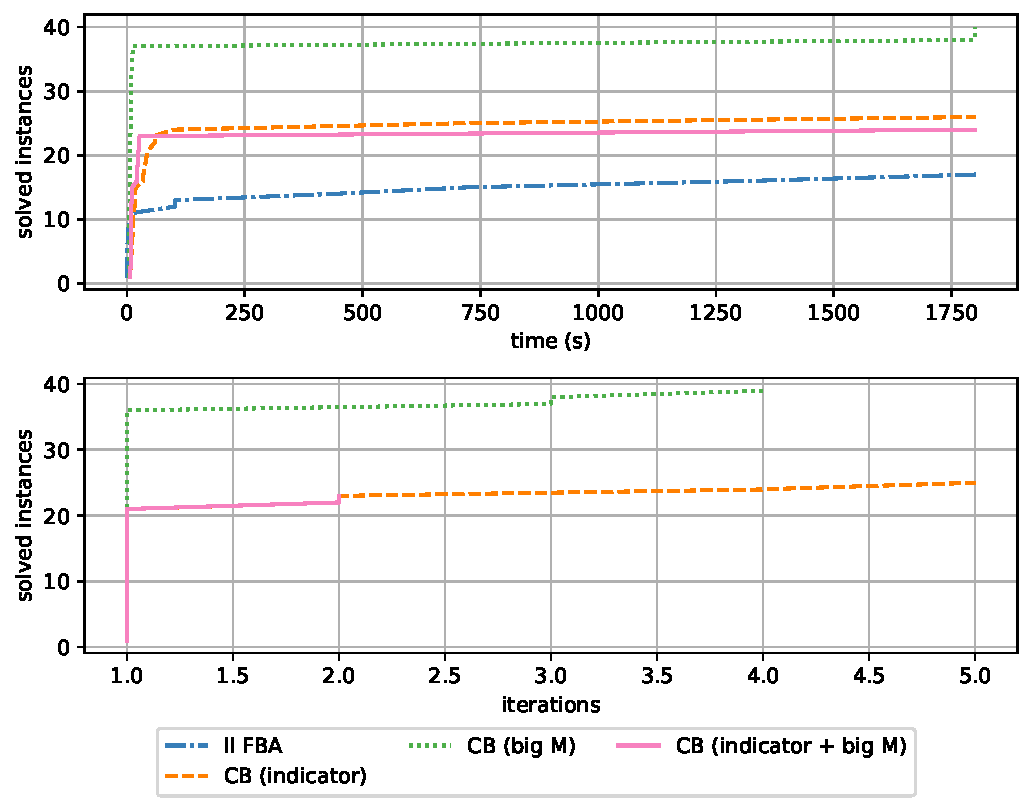
\includegraphics[width=0.8\textwidth]{Images/comparison_solved_instances_gecko_1.0e-8_indicator_and_big_m.pdf}
%     \label{fig:comparison_solved_instances_gecko_1.0e-8_indicator_and_big_m_as_MP}
% \end{figure}


%%%%%%%%%%%%%%%%%%%%%%%%%%%%
%%%%%Ende des Dokuments%%%%%
%%%%%%%%%%%%%%%%%%%%%%%%%%%%
\newpage
\restoreapp

\end{document} 